\documentclass{dstu3008/dstu3008}

% For printing use hardcopy option:
%\documentclass[hardcopy]{dstu3008/dstu3008}

\usepackage{tikz}
\usetikzlibrary{
    arrows,
    decorations.pathmorphing,
    backgrounds,
    positioning,
    fit,
    decorations.pathreplacing
}

% Condition whether Occupational Safety and Health (OSH) chapter is included.
% It's a dumb requirement by the university.
\newif\ifosh
\oshfalse  % To include OSH chapter use \oshtrue
\ifosh
    \newcommand{\osh}{% AUTHOR: Ruslan Kiianchuk <ruslan.kiianchuk@gmail.com>

\chapter{Labour protection and safety in emergencies}
\label{sec:labour}

PC users working conditions are analyzed for
their compliance with normative documents on safety engineering  and
sanitation. For retrieving and evaluating the influence of possible dangerous
or harmful production factors an interaction system
``Human--Machine--Environment'' (HME) is developed. Safety measures are
developed as the result of such system analysis.

\section{Analysis of the workplace working conditions}

The administrative building in which the workspace is located situates on the
first floor and has dimensions \sloppy{$6 \times 5.6 \times 3 \, \text{m}$}.

There are three workers in the office that use the following equipment:
\begin{itemize}
    \item Personal computer, 3 pieces;
    \item LCD monitor, 3 pieces.;
    \item Printer;
    \item Monitor.
\end{itemize}
The are also two windows 1.5~m wide and 1.7~m tall and doors 2.1~m tall and
0.9~m wide.
The analysis of the workspace indicates that the office has sufficient area
($6 \, \text{m}^2$) and volume ($20 \, \text{m}^2$) per worker and is compliant
with the sanity standard~\cite{dsanpin} for working with electronic computer
displays (figure~\ref{fig:workstation}).

The ``Human-Machine--Environment'' system (figure~\ref{fig:hme-graph}) is
created with the intention to retrieve possible dangerous and harmful
production factors~\cite{npaop4-12}. The list of H-M-E system connections is
shown in table~\ref{tbl:hme-legend}. Its main elements are:

\begin{description}
    \item[``Human''] --- staff that works in the office (2 workers);
    \item[``Machine''] --- electronic computers;
    \item[``Environment''] --- workspace environment;
    \item[``Product''] --- product of the algebraic cryptanalysis task solution.
\end{description}
Each element of the system contains three functional parts. Thereby the
``Human'' element is split by:
\begin{description}
    \item[$H_1$] --- execution of certain actions targeted on the main task solution;
    \item[$H_2$] --- human as a biological object influencing the environment;
    \item[$H_3$] --- human from the point of view of her psychophysiologic condition.
\end{description}
The main goal of the ``Machine'' element is influencing the product ---
execution of the primary technological function. Its auxiliary functions are to
generate particular environment parameters and execute emergency surveillance.
\begin{description}
    \item[$M_1$] --- execution of the primary technological function
        (performing computations using SAGE algebra system, construction and
        analysis of algebraic quadratic system that defines the GOST~28147-89
        cipher);
    \item[$M_2$] --- emergency protection support;
    \item[$M_3$] --- influencing the human and the environment.
\end{description}

\begin{figure}[htbp]
	\centering
    %&latex
% Copyright 2011 Zoresvit (c) <zoresvit@gmail.com>
% 
% 
%/

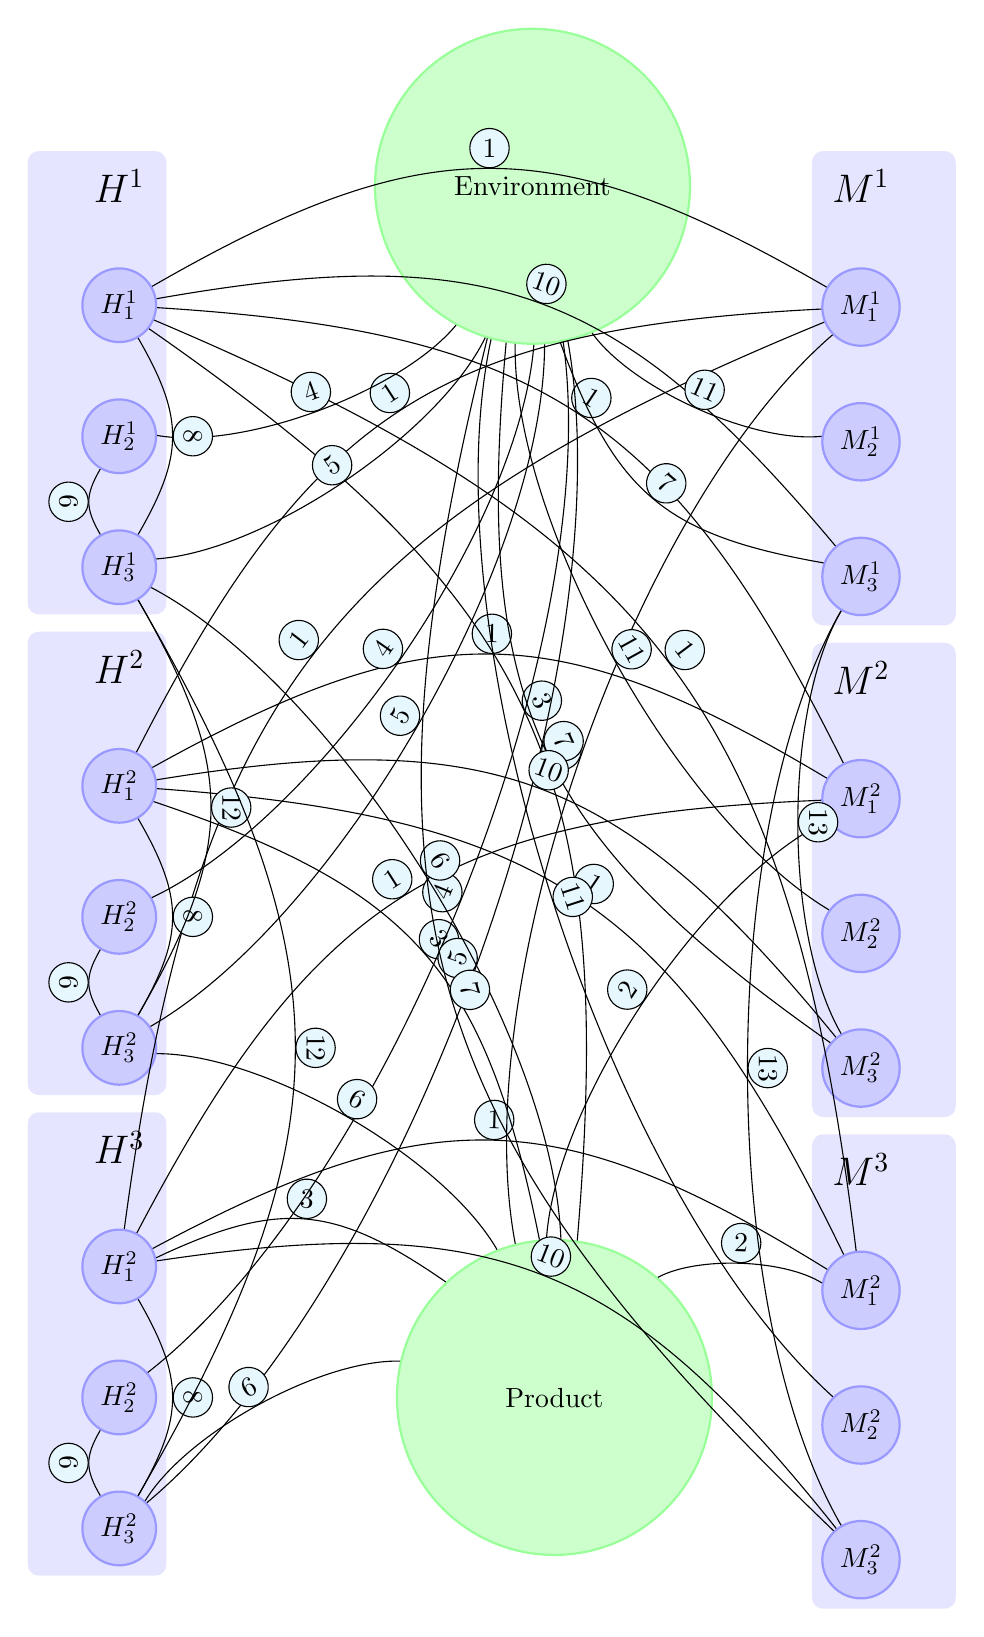
\begin{tikzpicture}
    \tikzstyle{func} = [node distance=7mm, circle, draw=blue!40, fill=blue!20, thick, minimum size = 8mm]
    \tikzstyle{elem} = [circle, draw=green!40, fill=green!20, thick, minimum size = 8mm]
    \tikzstyle{bound} = [node distance=1em]
    \tikzstyle{backfill} = [fill=blue!10, rounded corners]
    \tikzstyle{linkbelow} = [bend right, looseness=0.7]
    \tikzstyle{linkabove} = [bend left, looseness=1.2]
    \tikzstyle{linklabel} = [circle, fill=cyan!10, minimum size=5mm, inner sep=0, draw, above, sloped]

    \node (H1) [node distance=3ex] {\Large $H^1$};
    \node[func] (H11) [below=of H1]  {$H^1_1$};
    \node[func] (H12) [below=of H11] {$H^1_2$};
    \node[func] (H13) [below=of H12] {$H^1_3$};
    \node[bound] (H1bound) [left=of H1] {};

    \node (M1) [node distance=0.7\textwidth, right=of H1]  {\Large $M^1$};
    \node[func] (M11) [below=of M1]  {$M^1_1$};
    \node[func] (M12) [below=of M11] {$M^1_2$};
    \node[func] (M13) [below=of M12] {$M^1_3$};
    \node[bound] (M1bound) [right=of M1] {};

    \node (H2) [node distance=3ex, below=of H13] {\Large $H^2$};
    \node[func] (H21) [below=of H2]  {$H^2_1$};
    \node[func] (H22) [below=of H21] {$H^2_2$}; 
    \node[func] (H23) [below=of H22] {$H^2_3$}; 
    \node[bound] (H2bound) [left=of H2] {};

    \node (M2) [node distance=3ex, below=of M13]  {\Large $M^2$};
    \node[func] (M21) [below=of M2]  {$M^2_1$};
    \node[func] (M22) [below=of M21] {$M^2_2$};
    \node[func] (M23) [below=of M22] {$M^2_3$};
    \node[bound] (M2bound) [right=of M2] {};

    \node (H3) [node distance=3ex, below=of H23] {\Large $H^3$};
    \node[func] (H31) [below=of H3]  {$H^2_1$};
    \node[func] (H32) [below=of H31] {$H^2_2$}; 
    \node[func] (H33) [below=of H32] {$H^2_3$}; 
    \node[bound] (H3bound) [left=of H3] {};

    \node (M3) [node distance=3ex, below=of M23]  {\Large $M^3$};
    \node[func] (M31) [below=of M3]  {$M^2_1$};
    \node[func] (M32) [below=of M31] {$M^2_2$};
    \node[func] (M33) [below=of M32] {$M^2_3$};
    \node[bound] (M3bound) [right=of M3] {};

    \node[elem] (Env) [node distance=0.23\textwidth, minimum size=40mm, right=of H1] {Environment};
    \node[elem] (Prod) [node distance=0.25\textwidth, minimum size=40mm, right=of H32] {Product};


    \foreach \H / \M in {H11/M11, H11/M21, H11/M31, H21/M11, H21/M21, H21/M31, H31/M11, H31/M21, H31/M31}{
    \draw (\H) to [->, linkabove] node[linklabel]{1} (\M);
    }

    \foreach \M / \Prod in {M11/Prod, M21/Prod, M31/Prod}{
    \draw (\M) to [->, linkbelow] node[linklabel]{2} (\Prod) ;
    }

    \foreach \H / \Prod in {H11/Prod, H21/Prod, H31/Prod}{
    \draw (\H) to [<->, linkabove] node[linklabel]{3} (\Prod);
    }

    \foreach \H / \Env in {H12/Env, H22/Env, H32/Env}{
    \draw (\H) to [->, linkbelow] node[linklabel]{4} (\Env);
    }

    \foreach \Env / \H in {Env/H13, Env/H23, Env/H33}{
    \draw (\H) to [<-, linkbelow] node[linklabel]{5} (\Env);
    }

    \foreach \Prod / \H in {Prod/H13, Prod/H23, Prod/H33}{
    \draw (\Prod) to [->, linkbelow] node[linklabel]{6} (\H);
    }

    \foreach \M / \Env in {M13/Env, M23/Env, M33/Env}{
    \draw (\M) to [->, linkabove] node[linklabel]{7} (\Env);
    }

    \foreach \Hact / \Hpsy in {H11/H13, H21/H23, H31/H33}{
    \draw (\Hact) to [->, linkabove] node[linklabel]{8} (\Hpsy);
    }

    \foreach \Hpsy / \Hbio in {H13/H12, H23/H22, H33/H32}{
    \draw (\Hpsy) to [->, linkabove] node[linklabel]{9} (\Hbio);
    }

    \foreach \H / \M in {H11/M13, H21/M23, H31/M33}{
    \draw (\H) to [->, linkabove] node[linklabel]{10} (\M);
    }

    \foreach \Env / \M in {Env/M12, Env/M22, Env/M32}{
    \draw (\Env) to [->, linkbelow] node[linklabel]{11} (\M);
    }

    \draw (H13) to [<->, linkabove] node[linklabel]{12} (H23);
    \draw (H13) to [<->, linkabove] node[linklabel]{12} (H33);
    \draw (M13) to [<->, linkbelow] node[linklabel]{13} (M23);
    \draw (M13) to [<->, linkbelow] node[linklabel]{13} (M33);

    \begin{pgfonlayer}{background}
        \node [backfill, fit= (H1) (H11) (H12) (H13) (H1bound)] {};
        \node [backfill, fit= (M1) (M11) (M12) (M13) (M1bound)] {};
        \node [backfill, fit= (H2) (H21) (H22) (H23) (H2bound)] {};
        \node [backfill, fit= (M2) (M21) (M22) (M23) (M2bound)] {};
        \node [backfill, fit= (H3) (H31) (H32) (H33) (H3bound)] {};
        \node [backfill, fit= (M3) (M31) (M32) (M33) (M3bound)] {};
    \end{pgfonlayer}
\end{tikzpicture}


	\caption{H-M-E system scheme}
	\label{fig:hme-graph}
\end{figure}

\begin{longtable}{|p{0.09\textwidth}|p{0.16\textwidth}|p{0.66\textwidth}|}
\caption{Human--Machine--Enviroment system connections} \label{tbl:hme-legend} \\ \hline
\begin{center} Index \end{center} & Connection direction & \begin{center} Essence of the connections \end{center} \\ \hline
\endfirsthead
\multicolumn{3}{l}{\hfill Proceeding table \thechapter.\arabic{table}}
\endhead
    1 & $H_1 \rightarrow M_1$ & Human controls equipment providing its correct
    functioning (operating on computer using peripheral input devices).  \\ \hline
    2 & $M_1 \rightarrow \text{Prod}$ & Machine influence on the product
    (construction of the cryptographic transformation model, research
    computations). \\ \hline
    3 & $H_1 \leftrightarrow \text{Prod}$ & Human influence on the product and
    backwards (human is the source of ideas that defines needed actions during
    the work and analysis the working process; depending on the project
    complexity and accomplishment success causes mental strain for the
    workers). \\ \hline
    4 & $H_2 \rightarrow \text{Env}$ & Human influence on the environment
    (generation of heat and humidity, temperature increase). \\ \hline
    5 & $\text{Env} \rightarrow H_3$ & Environment influence on human health
    (the psychophysiologic condition working capacity depends on the
    environment conditions). \\ \hline
    6 & $\text{Prod} \rightarrow H_3$ & Product influence on human (complexity
    and execution progress of the primary task influence the human physical
    condition). \\ \hline
    7 & $M_3 \rightarrow \text{Env}$ & Machine influence on environment
    (computer is the source of increased temperature, noise, ionizing and
    electromagnetic emission). \\ \hline
    8 & $H_1 \rightarrow H_3$ & The working activity influences
    human psychophysiologic condition (human psychophysiologic condition
    depends on the success and amount of the completed work). \\ \hline

    9 & $H_3 \rightarrow H_2$ & Influence of psychophysiologic condition on
    human biological processes density (fatigue, irritability, euphoria). \\ \hline
    10 & $H_1 \rightarrow M_3$ &
    Human control of the machine influence on environment (normalization of
    harmful emission, humidity and temperature control). \\ \hline
    11 & $\text{Env} \rightarrow M_2$ & Environment influence on emergency
    protection abilities (unfavourable environment parameters may lead to
    insufficient emergency protection). \\ \hline
    12 & $H^*_3 \leftrightarrow H^*_3$ & Reciprocal influence of each human's
    psychophysiologic conditions. \\ \hline
    13 & $M^*_1 \leftrightarrow M^*_1$ & Mutual influence of machine side
    emissions. \\ \hline
\end{longtable}

Based on the analysed connections harmful and dangerous production factors may
be retrieved according to~\cite{gost003}. The following harmful factors are
found:
\begin{itemize}
    \item physical:
        \begin{enumerate}
            \item increased electromagnetic emission;
            \item increased equipment surface temperature;
            \item reduced air humidity;
        \end{enumerate}
    \item chemical: absent;
    \item biological: absent;
    \item psychophysiologic:
        \begin{enumerate}
            \item mental overstress;
            \item overstress of analyzers.
        \end{enumerate}
\end{itemize}
Reduced air humidity is the dominant harmful factor.


\begin{longtable}{|p{0.35\textwidth}|p{0.09\textwidth}|p{0.09\textwidth}|c|c|c|p{0.12\textwidth}|}
\caption{Evaluation for factors of working environment} \label{tbl:hme-legend} \\ \hline
\begin{center} Factors \end{center} & \begin{center}Norm\end{center} & \begin{center} Fact \end{center} & 1 st. & 2 st. & 3 st. & duration, \% for working shift\\ \hline
\endfirsthead
\multicolumn{7}{l}{\hfill Proceeding table \thechapter.\arabic{table}}
\endhead
Noise & 50 & 49 &  &  &  & 93 \\ \hline
Non-ionising radiation & & &  &  &  & \\ \hline
5~Hz -- 2~kHz & 25 & less 25 &  &  & & 93 \\ \hline
2~kHz -- 400~kHz & 2.5 & less 2.5 &  &  & & 93 \\ \hline
X-ray radiation & less 100 & 14 &  &  & & 93 \\ \hline
Micro climate & & &  &  & & \\ \hline
Air temp. & 22-24\newline 23-25 & 31.5 &  & + & &  100 \\ \hline
Air movement & 0.1\newline 0.1 & less 0.1 &  &  & &  100 \\ \hline
Relative humidity& 60-40\newline 60-40 & less 65 &  &  & &  100 \\ \hline
Light & & &  &  & &  \\ \hline
Natural & 1.2 & 1.2 &  &  & & 93 \\ \hline
Artificial light & 200-500 & 370 &  &  & & 93 \\ \hline
Work intensity & & &  &  & & \\ \hline
Attention & & &  &  & & \\ \hline
Duration of concentration & 25-50 & 48 &  &  & & 48 \\ \hline
Signals density & 75-175 & less 75 &  &  & & 93 \\ \hline
Density of analyzers & & &  &  & & \\ \hline
Eyesight & 2-3 & 3 &  &  & & 93 \\ \hline
Hearing & unders. words 70--90~\% & 3 &  &  & & 93 \\ \hline
 Emot. \& Intel. density & Resp. for func. quality & Resp. for perform.  tasks &  &  & & 93 \\ \hline
Repetitive routines &  & &  &  & & \\ \hline
Repetitive tasks & 100-25 & 100-25 &  &  & & 93 \\ \hline
Observ. process & 46-80 & 80 &  &  & & 80 \\ \hline
Shifts & & day &  &  & & \\ \hline
No. fuctors & 9 &  &  &  & & \\ \hline
\end{longtable}

The exceeding factor is air temperature. During the working process of the staff
because of heat emission the temperature raises to $31.5^\circ$~C (3 cl. 2 st.)
and is harmful for health of the staff. For normalizing the air temperature
conditioning system must be set up with precomputed parameters.

\section{Industrial security in production building}
Considering the electrical equipment located in the office, organizational and
technical countermeasures for protecting workers' safety need to be applied.
The workspace belongs to the class of increased fire threat according
to~\cite{npaop1-21}.

The building power supply is three-phased four-wired electric network with
dead-earthed neutral, alternating current, 50~Hz frequency and $380/220$~V
voltage. Neutral grounding of the equipment is done for providing electrical
security according to~\cite{gost030}. The current threshold for automatic
overload control exceeds the maximum equipment current consumption 5 times.
Triggering time of the overload controller does not exceed 0.2~s.

\section{Labour health at the workplace}

According to~\cite{dsanpin} microclimate the standards for given room that
corresponds to power inputs category \verb+Ia+ are shown in
table~\ref{tbl:aero-req}.

\begin{table}[htbp]
    \centering
    \caption{Microclimate standards}
    \label{tbl:aero-req}
    \begin{tabular}{|l|l|l|l|}
        \hline
        Season & Air temp., $^\circ$C & Rel. humid., \% & Air movement, m/s\\ \hline
       Cold & 22-24 & 60-40 & 0.1 \\ \hline
       Hot & 23-25 & 60-40 & 0.1 \\ \hline
    \end{tabular}
\end{table}

For providing the expected climate conditions an air conditioning system needs
to be set up in the room. For computing the required parameters of air
conditioning system on needs to compute the heat coming into the room from
sunlight, artificial light, humans and equipment.

Sources of heat are split into:
\begin{description}
    \item[$Q_1$] --- heating from environment;
    \item[$Q_2$] --- heating from humans;
    \item[$Q_3$] --- heating from equipment.
\end{description}
Overall heating is computed by the formula $Q = Q_1 + Q_2 + Q_3$. Input heat
from environment is computed as follows:
\begin{equation}
Q_1 = (S \cdot h \cdot q) / 1000,
\end{equation}

where $S$ -- room area, $h$ -- height of the room, $q$ -- load unit (when mean
lightning is 35~W/$m^2$). Heat income from humans is estimated as 0.13~kW. Heat
income from a PC is estimated in 0.3~kW. Heating income from printer is
neglectful. According to these factors the overall heating input equals:
\begin{equation}
Q = Q_1 + Q_2 + Q_3 = (33.6 \cdot 3 \cdot 35) / 1000 + 0.13 \cdot 3 + 0.3 \cdot
3 = 4.87\text{~kW}\enspace.
\end{equation}

Power of conditioning system must be in the range $-5\%$ -- $+15\%$ from
computed power $Q$. So in order to provide the required climate conditions in
the room the conditioning system with power 4.87~kW must be installed. According
to conditioning power catalogue the most satisfying model is Panasonic
CS-E18MKDW with power of 5~kW.

\begin{figure}[htbp]
    \centering
    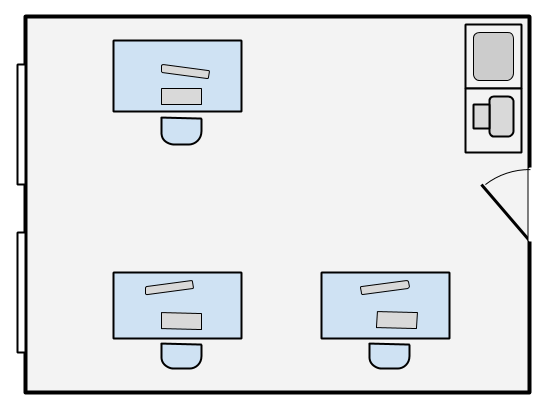
\includegraphics[scale=0.5]{images/workstation}
    \caption{Workstations location in the room}
    \label{fig:workstation}
\end{figure}

\section{Fire safety of the production building}
Solid ignitable materials are used in the room, the building has brick walls
and armoured concrete floor. Therefore the building belongs to 2-nd fire
resistance ratio according to~\cite{dbn_b11}, production belongs to category B
of flammability and explosion risk according to~\cite{napb002}.

Pursuant to~NAPB B.03.001-2004 the building must have two fire extinguishers with
up to 6~kg of reactant or one fire extinguisher with at least 8~kg of reactant.
Any type of fire extinguishers fits for the category B building.

Evacuation plans that are located in every room and in corridors allow to
efficiently leave the building in case of fire through the main exit of
 $1.9 \, \text{m}$ hight and $1.2 \, \text{m}$ wide. Two employees work at the
 office with area of $25 \, \text{m}^2$. Therefore no extra emergency exit is
 needed. The fire and explosion safety requirements are satisfied.


}
\else
    \newcommand{\osh}{}
\fi

\newcommand{\misty}{\mbox{MISTY1}}
\newcommand{\gost}{\mbox{GOST~28147-89}}
\newcommand{\thesisAuthor}{Ruslan I. Kiyanchuk}
\newcommand{\thesisTitle}{Cryptographic properties analysis of perspective symmetric transformations}

\hypersetup{
    pdfauthor = {\thesisAuthor},
    pdftitle = {\thesisTitle},
 }


\title{\thesisTitle}
\author{\thesisAuthor}


\begin{document}

% AUTHOR: Ruslan Kiianchuk <ruslan.kiianchuk@gmail.com>
% Masters diploma title.

\thispagestyle{empty}
\begin{center}
    Міністерство освіти і науки України \\[1ex]
    Харківський національний університет радіоелектроніки \\[1ex]
    Факультет Комп'ютерної інженерії та управління \\[1ex]
    Кафедра Безпеки інформаційних технологій \\[2ex]
    \MakeUppercase{Магістерська робота} \\[4ex]
    \MakeUppercase{Пояснювальна записка} \\[1ex]

    \MakeUppercase{ГЮІК ХХХХХХ.551.07 ПЗ} \\[-2ex]
    \line(1, 0){450} \\[-2ex]
    {\scriptsize (позначення документу)} \\[2ex]

    Аналіз криптографічних властивостей перспективних симетричних перетворень \\[-2ex]
    \line(1, 0){450} \\[-2ex]
    {\scriptsize (тема роботи)} \\[2ex]

    \begin{tabular}{
        p{0.13\textwidth}
        >{\centering\arraybackslash}p{0.2\textwidth}
        >{\centering\arraybackslash}p{0.005\textwidth}
        >{\centering\arraybackslash}p{0.1\textwidth}
        >{\centering\arraybackslash}p{0.005\textwidth}
        >{\centering\arraybackslash}p{0.30\textwidth}}
        Студент & БІКСм-12-1 & & & & Кіянчук~Р.~І. \\ \cline{2-2}\cline{4-4}\cline{6-6} \\[-4ex]
        & {\scriptsize (група)} & & {\scriptsize (підпис)} & & {\scriptsize (прізвище, ініціали)} \\[1ex]
        \multicolumn{2}{p{0.4\textwidth}}{Керівник дипломної роботи} & & & & доц.~Олійников~Р.~В. \\ \cline{4-4}\cline{6-6} \\[-4ex]
        & & & {\scriptsize (підпис)} & & {\scriptsize (посада, прізвище, ініціали)} \\
        Консультанти: & & & & & \\[1ex]
        \multicolumn{2}{p{0.4\textwidth}}{Зі спецчастини} & & & & доц.~Олійников~Р.~В. \\ \cline{4-4}\cline{6-6} \\[-4ex]
        & & & {\scriptsize (підпис)} & & {\scriptsize (посада, прізвище, ініціали)} \\[1ex]
        \multicolumn{2}{p{0.4\textwidth}}{З розділу ОП} & & & & ст.~викл.~Сердюк~Н.~М. \\ \cline{4-4}\cline{6-6} \\[-4ex]
        & & & {\scriptsize (підпис)} & & {\scriptsize (посада, прізвище, ініціали)} \\[1ex]
        \end{tabular}

        \vfill
        \begin{flushleft}
            \hspace{4ex}Допускається до захисту \\[1ex]
        \end{flushleft}
        \begin{tabular}{
            p{0.2\textwidth}
            >{\centering\arraybackslash}p{0.15\textwidth}
            >{\centering\arraybackslash}p{0.005\textwidth}
            >{\centering\arraybackslash}p{0.1\textwidth}
            >{\centering\arraybackslash}p{0.005\textwidth}
            >{\centering\arraybackslash}p{0.3\textwidth}}
            \mbox{Зав. кафедрою} & БІТ & & & & проф. Горбенко~І.~Д. \\ \cline{2-2}\cline{4-4}\cline{6-6} \\[-4ex]
                                       & & & {\scriptsize (підпис)} & & {\scriptsize (прізвище, ініціали)} \\[1ex]
        \end{tabular}
        \vfill
        2013~р.
    \end{center}
    \clearpage

\setcounter{page}{4}

\newpage
% Creative Commons License.
\begin{center}
\leavevmode

\includegraphics[width=1in]{images/cc-by.png}
\label{fig:cc}
\end{center}
\begin{center}
%insert a link to the licence and its description below
This thesis is licensed under a \\
\href{http://creativecommons.org/licenses/by/4.0/}
{Creative Commons Attribution 4.0 International License.}
\end{center}
\newpage


% AUTHOR: Ruslan Kiianchuk <ruslan.kiianchuk@gmail.com>

\selectlanguage{ukrainian}
\begin{abstract}
    Магістерська робота містить \pageref{LastPage}~сторінок, \totfig~рисунок,
    \tottab~таблиць, \totapp~додатків та \totref~джерел.

    У роботі представлено аналіз перспективних симетричних шифрів, що є
    стандартами на державному та міжнародному рівні.

    Розроблено методи побудови системи нелінійних рівнянь низького степеня від
    багатьох невідомих, що описують криптоалгоритми \misty\ та
    ГОСТ~28147-89. Представлено характеристики алгебраїчної системи
    рівнянь кожного шифру та їх порівняння з аналогічними системами рівнянь
    для криптоалгоритмів AES, Camellia та PRESENT.

    Оцінено криптографічну стійкість шифрів \mbox{ГОСТ~28147-89} та \misty\ до
    алгебраїчного криптоаналізу. Здійснено алгебраїчну атаку на зменшені версії
    криптоалгоритмів використовуючи методи SAT-solver для вирішення системи
    нелінійних рівнянь та відновлення ключа шифрування.

    \keywords{симетричні шифри, \misty, ГОСТ~28147-89, алгебраїчний криптоаналіз}
\end{abstract}

\clearpage
\selectlanguage{english}
\begin{abstract}
    This thesis contains \pageref{LastPage}~pages, \totfig~figures,
    \tottab~tables, \totapp~appendices and \totref~references.

    The work presents analysis of symmetric block ciphers that are adopted
    standards on country and international levels.

    Methods for constructing non-linear multivariate quadratic (MQ) equations
    systems that define cryptoalgorithms \misty\ and \gost\ are developed.
    Characteristics for each algebraic system are presented and compared to
    analogous systems for cryptoalgorithms AES, DES and PRESENT.

    Further the strength of \gost\ and \misty\ ciphers to algebraic
    cryptanalysis is researched. Algebraic attack on reduced rounds versions of
    the ciphers is executed using SAT-solver methods for solving non-linear
    equations systems and recovering the enciphering key.

    \keywords{symmetric ciphers, algebraic cryptanalysis, \misty, \gost}
\end{abstract}
\clearpage

\tableofcontents
% AUTHOR: Ruslan Kiianchuk <ruslan.kiianchuk@gmail.com>

\addcontentsline{toc}{Chapter}{\texorpdfstring{\MakeUppercase{List of abbreviations}}{}}

\nomenclature{3G}{Third generation of mobile telecommunications technology}
\nomenclature{3GPP}{The third generation partnership project}
\nomenclature{ANF}{Algebraic normal form}
\nomenclature{CNF}{Conjunctive normal form}
\nomenclature{FCSR}{Feedback with carry shift register}
\nomenclature{GE}{Gate equivalents}
\nomenclature{GSM}{Global System for Mobile Communications}
\nomenclature{LFSR}{Linear feedback shift register}
\nomenclature{XOR}{Exclusive or}
\nomenclature{NLFSR}{Non-linear feedback shift registers}
\nomenclature{SPN}{Substitution-permutation network}
\nomenclature{LTE}{Long Term Evolution, a standard for wireless communication}
\nomenclature{UMTS}{Universal Mobile Telecommunications System}
\nomenclature{IV}{Initialization vector}
\nomenclature{UEA}{UMTS Encryption Algorithm}
\nomenclature{UIA}{UMTS Integrity Algorithm}
\nomenclature{FSM}{Finite state machine}
\nomenclature{MQ}{Multivariate quadratic system}
\nomenclature{SAT}{Satisfiability (denoting boolean satisfiability problem)}
\nomenclature{ISO}{International Organization for Standardization}
\nomenclature{ECB}{Electronics codebook mode}
\nomenclature{CBC}{Cipher block chaining mode}
\nomenclature{CFB}{Cipher feedback mode}
\nomenclature{OFB}{Output feedback mode}
\nomenclature{IV}{Initialization vector}
\nomenclature{CIS}{Commonwealth of Independent States}
\nomenclature{BR}{Bit reorganization layer in ZUC stream cipher}
\nomenclature{AES}{Advanced Encryption Standard}
\nomenclature{SDU}{System data unit}
\nomenclature{RFC}{Request for Comments}

\printnomenclature
\clearpage

% AUTHOR: Ruslan Kiianchuk <ruslan.kiianchuk@gmail.com>

\Chapter{Introduction}
\label{sec:intro}

Symmetric cryptographic transformations are known to be the only effective
method of providing data confidentiality and integrity in all fields of
communication technologies~\cite{moldovyan2007innovative}. They need to be not
only cryptographically strong, but also have high performance and low resources
consumption to satisfy modern needs for securing information. Consequently,
robust requirements on cryptographic security, lightweight implementation and
performance are entrusted to such transformations.

Symmetric ciphers came through a long history of development and improvement
from the most primitive schemes based on symbols substitution and disk
encryptors to advanced mathematical algorithms following Kerckhoffs'
principle~\cite{kahn1996codebreakers}.
A tremendous contribution to enciphering theory has been done by Claude
Shannon's work~\cite{shannon:secrecy} back in 1949. He introduced the
fundamentals of information theory and made it possible to evaluate and
mathematically prove cipher security. Ubiquitous computerization, mass
deployment of pervasive devices and extensive Internet access caused
cryptography to find comprehensive applications in information systems. Despite
the advanced mathematics behind modern cryptoalgorithms, real operating
security systems often have weaknesses due to incorrect usage or implementation
errors.

Security of mobile communication systems fell far behind from what was
state-of-the-art in modern cryptography. The A5/1 cipher used in GSM standard
for over 10 years can be broken within seconds using a combined distributed
rainbow table code book to decrypt GSM voice calls and text
messages~\cite{secproject}.
Communication over satellite phones has also been shown to be insecure after
reverse engineering the proprietary ciphers \mbox{GMR-1} and \mbox{GMR-2}.
\mbox{GMR-1} is a variant of A5/2 cipher (which is prohibited for
implementation in mobile phones as of July 2007) and is vulnerable to a known
ciphertext-only attack with an average case complexity of
$2^{32}$~\cite{3gpp:a52:2007}.
\mbox{GMR-2} is an original cipher, but its session key can be recovered with
65 bytes of keystream at a moderate computational
complexity~\cite{kiyanchuk:zuc}.

In~\cite{cryptoeprint-2010-013} an effective attack on KASUMI cipher
\footnote{KASUMI cipher is adopted by 3GPP as A5/3 cryptographic algorithm
for securing mobile communications.}
used in 3G systems is presented. Key recovery for the full cipher was done in
hours on low-end computer that used unoptimized cipher reference implementation.
It is worth noting that KASUMI is based on MISTY cryptoalgorithm which however
could not be broken by the same attack. Therefore even slight modifications to
robust cipher may significantly impact the security of the algorithm.

The need of deep analysis and public evaluation of cryptographic algorithms
before deploying them into real systems is obvious. Several ciphers are
considered for becoming worldwide standards in the field of providing data
confidentiality at the moment.

\misty\ is a symmetric block cipher designed in 1995 which has been one of the
selected algorithms in the European NESSIE project~\cite{Preneel_neweuropean}
and recommended for Japaneese government use~\cite{cryptrec:misty}. Though no
vulnerabilities have yet been found in \misty\ cipher, some of its successors
were broken (KASUMI) or provided with a theoretical attack (Camellia) which may
be feasible in future with increase of computations
power~\cite{Biryukov03decanniere}.

\gost\ is a legacy cipher that has been a subject to cryptanalysis for more than
20 years. Despite its wide usage in Ukraine and other CIS countries since the
publication in 1990, the cipher has been proposed for international
standardization only in 2010, but hasn't been accepted
however~\cite{isoiec-18033}. Therefore a detailed security evaluation and
properties analysis of these ciphers are essential to validate their pervasive
deployment into security systems.

\osh{
    Chapter~\ref{sec:labour} analyses PC users working conditions and
    their compliance with normative documents on safety engineering  and
    sanitation. For retrieving and evaluating the influence of possible dangerous
    or harmful production factors an interaction system
    ``Human--Machine--Environment'' (HME) is developed. Safety measures are
    developed as the result of such system analysis.
}

% AUTHOR: Ruslan Kiianchuk <ruslan.kiianchuk@gmail.com>
%

\chapter{State of art analysis and synthesis of symmetric cryptographic transformations}
\label{sec:symmetry_review}

Evaluation and design rationale are essential parts of developing and
deploying  the considered cryptographic security system. The primary goal of
cryptography is to design mathematical methods for providing security against
adversary's malicious actions under any predetermined conditions.

However, as practice shows, it's unfeasible to take into account all possible
attacks that may be invented in the future due to technological and scientific
innovations during the development stage. Therefore, the most widespread
method for analysing computationally strong cryptographic primitives is
complexity evaluation of every known applicable attack.

\section{Classification of attacks on symmetric ciphers}

Attacks on symmetric ciphers are defined by the abilities and data
that an adversary can operate with. Most of them refer actions that may be
done to cipher entities such as plaintexts and ciphertexts, however a separate
class of attacks that exploits cipher implementation rather than the
algorithm itself exists.

A ciphertext-only attack leaves the adversary with a set of ciphertexts that
she
\footnote{Following the tradition started by Shafi Goldwasser in her Lecture
Notes on Cryptography, ``she'' is used throughout the text as referring to a
subject of unknown gender.}
can use to recover the corresponding plaintext or encryption key. Such
conditions are the most complex for cryptanalyst. In a known plaintext attack
the adversary has a fixed set of plaintext and ciphertext
pairs~\cite{menezes:applied_cryptography}.

In chosen plaintext and chosen ciphertext attacks the adversary gets an
ability to encrypt plaintexts or decrypt ciphertexts of her choice
respectively. So the cipher needs to have such plaintext and ciphertext
spaces that would make it infeasible for the attacker to get full dictionary of
all possible plaintexts and corresponding
ciphertexts~\cite{menezes:applied_cryptography}.

Related key attacks exploits possible relations between encryption keys to
break the cryptographic system~\cite{StampLow:AppliedCryptanalysis}.

Side channel attacks are somewhat outside of mathematical attacks scope. They
use some cipher implementation peculiarities to gain information about the
encryption key observing the cryptographic system during operation. So far no
mathematical countermeasures exist that would guarantee the security of the
transformation against these types of attacks ~\cite{Quisquater:sidechannel}.

A cipher is considered to be insecure if any type of attack exists that allows
to get some information about the key with a complexity lower than a brute
force.

\section{Block ciphers}

A block cipher is a function which maps $n$-bit plaintext blocks to $n$-bit
ciphertext blocks, parameterized by a $k$-bit key
$K$~\cite{menezes:applied_cryptography}. Here $n$ is called the blocklength.
The encryption key $K$ has to be random. In order to always provide unique and
correct decryption the mapping function defined by a chosen key must be
bijective.

A straightforward usage of a block cipher to encrypt separate blocks of data may have
disadvantage in many applications. Consequently, several block cipher modes of
operations have been developed to satisfy various security purposes.

\subsection{Algebraic representation}
\label{sec:block-algebraic}

A symmetric block cipher may be represented as an algebraic
system~\cite{babash:cryptography}
\begin{equation}
\label{eqn:block-algebraic}
\Sigma_{A} = \left< X, K, Y, E, D \right> \enspace,
\end{equation}

    where $X$ is a plaintext space defined over finite alphabet $Q_X$, \\
$K$ --- a key set (usually defined by fixed length strings over $Q_X$), \\
$Y$ --- ciphertext space defined over finite alphabet $Q_Y$, \\
$E: X \times K \rightarrow Y$ --- a set of enciphering rules based on
parametrized maps $e_k(x) = y$ for which $k \in K$, $x \in X$, $y \in Y$. \\
Mappings $e_k(\cdot)$ and $d_k(\cdot)$ for any $k \in K$  are bijective and
ensure satisfaction of both conditions $d_k(e_k(x)) = x$ and $e_k(d_k(y)) = y$.
Plaintext and ciphertext spaces of all widespread modern symmetric ciphers
coincide ($Q_X = Q_Y$), so such ciphers are therefore endomorphic, that is
\mbox{$X = Y$}.
For cryptographically secure ciphers the sets of encrypting and decrypting
rules must have random mapping properties, and $e_k(\cdot)$, $d_k(\cdot)$ must
be random permutations.


\subsection{Modes of operation}

Simple encryption of data chunks block-by-block is called an electronics
codebook mode (ECB). As seen from figure~\ref{fig:mode-ecb} each plaintext is
encrypted independently. Error propagation is limited within one block, but
this mode is insecure for enciphering large correlated
data~\cite{menezes:applied_cryptography}.
\begin{figure}[htbp]
	\centering
	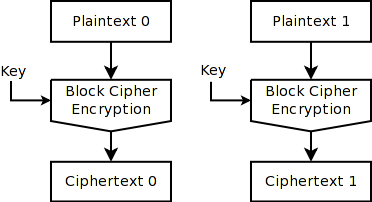
\includegraphics[scale=0.6]{images/modes_ecb}
	\caption{ECB mode of operation}
	\label{fig:mode-ecb}
\end{figure}

Cipher block chaining mode (CBC) is represented on figure~\ref{fig:mode-cbc}.
In CBC mode two identical plaintext do not encrypt to the same ciphertext as
the encryption depend on the initialization vector (IV) and two previous blocks
instead. This causes error propagation in ciphertext expand to two blocks, but
modifications to plaintext influence all subsequent blocks and make correct
decryption impossible. Such encryption mode is also more secure for enciphering
correlated data~\cite{menezes:applied_cryptography}.

Cipher feedback mode (CFB) shown on figure~\ref{fig:mode-cfb} turns a block
cipher into self-synchronizing
(see section \ref{sec:stream_ciphers_classification}) stream cipher.
\begin{figure}[htbp]
	\centering
	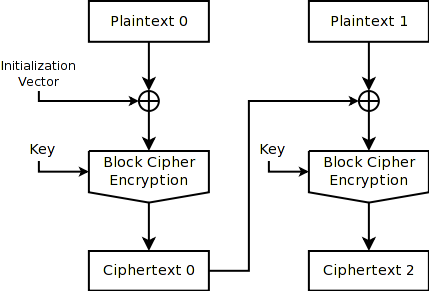
\includegraphics[scale=0.6]{images/modes_cbc}
	\caption{CBC mode of operation}
	\label{fig:mode-cbc}
\end{figure}
\begin{figure}[htbp]
	\centering
	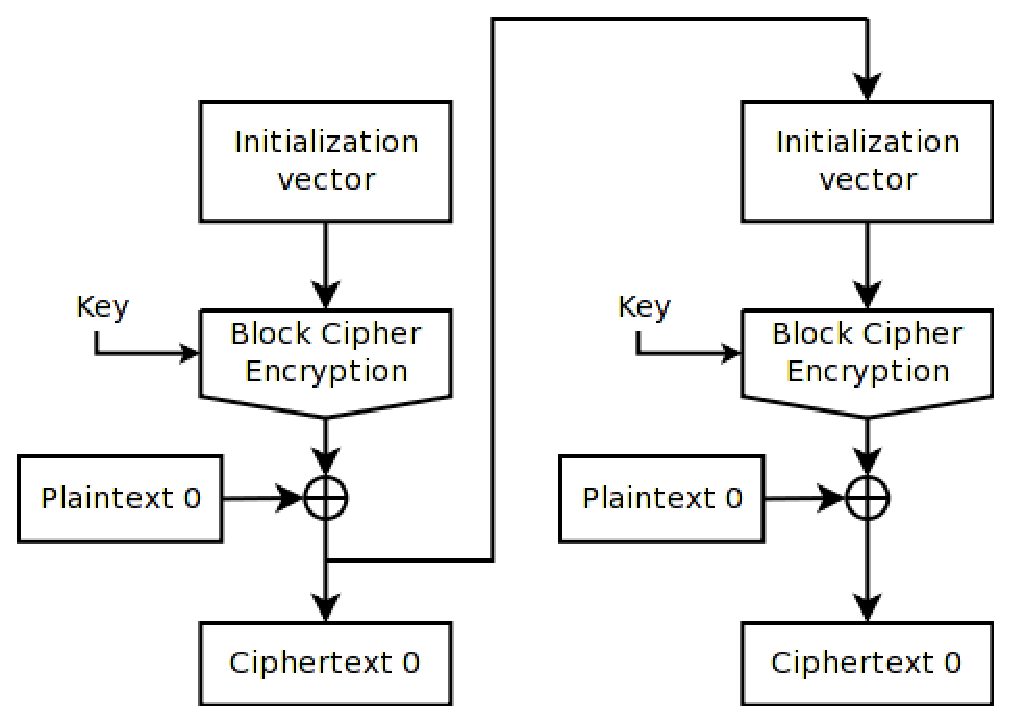
\includegraphics[scale=0.6]{images/modes_cfb}
	\caption{CFB mode of operation}
	\label{fig:mode-cfb}
\end{figure}

Output feedback mode (OFB) is similar to CFB (figure~\ref{fig:mode-ofb}) and
differs only by a feedback connection.
\begin{figure}[htbp]
	\centering
	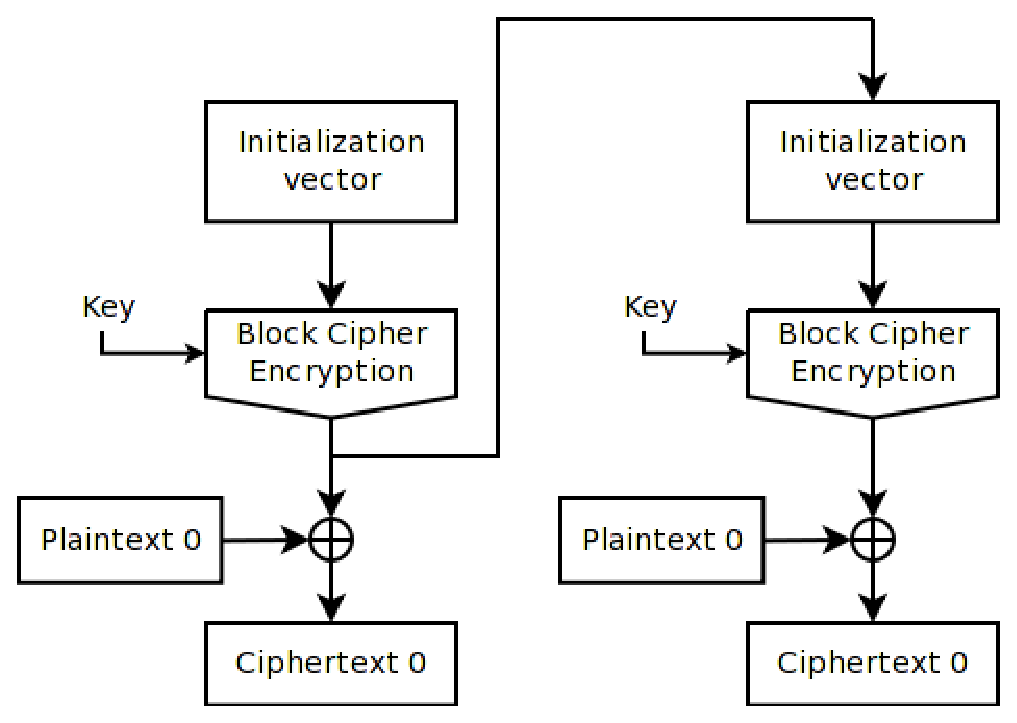
\includegraphics[scale=0.6]{images/modes_ofb}
	\caption{OFB mode of operation}
	\label{fig:mode-ofb}
\end{figure}
The main advantages of this mode is
absence of error propagation (since keystream generation doesn't depend on the
plaintext) and parallel processing capability.

\section{Stream ciphers}

The distinct difference between stream ciphers and block ciphers was for the
first time defined by Rainer Rueppel~\cite{robshaw:rsa:streamciphers}:

``Block ciphers operate with a fixed transformation on large blocks of
plaintext data; stream ciphers operate with a time-varying transformation on
individual plaintext digits''.

Stream ciphers gained great progress since Shannon's analysis of the
Vernam cipher where he proved it to be theoretically
unbreakable~\cite{shannon:secrecy}. However such cryptosystems were complex and
unprofitable to implement because of the need of secret channel to exchange key
material which was the size of the message itself.

Trying to overcome disadvantages of the Vernam cryptosystem, stream ciphers
inherit its idea, but use short key instead to generate a pseudo-random sequence
of needed length. That is, plaintext is encrypted into ciphertext with
pseudo-random sequence,  called the keystream, which is produced by a finite
state automaton whose initial state is determined by a secret key. Therefore
stream ciphers require high structural secrecy in order to be cryptographically
strong.

Stream ciphers are fast and well suited for hardware though some
cryptoalgorithms designed for efficient software implementation exist. They are
generally used in cases of continuous or unknown amount of data to be encrypted
and strict buffering constraints.

\subsection{Classification}
\label{sec:stream_ciphers_classification}

Depending on the choice of how the next state of cryptosystem is generated from
the current state, two types of stream ciphers are distinguished: synchronous
and self-synchronizing (or asynchronous)~\cite{menezes:applied_cryptography}.

In synchronous stream ciphers the next state of the automaton is independent of
plaintext and ciphertext. Such ciphers have no error-propagation and
consequently don't detect errors during decryption. This fact allows an attacker
to inconspicuously alter ciphertext which will be successfully decrypted to a
different plaintext. Another significance consists in the fact that encrypting
and decrypting devices must constantly stay synchronized. Otherwise the
decryption will fail.

Asynchronous stream ciphers are able to resume correct decryption in case
transmitter and receiver fall unsynchronized. Error-propagation is limited to
the state bits that depend on previously generated ciphertexts. Such ciphers are
difficult for analysis because the keystream depends on input message. They
are also vulnerable to playback attack: if an attacker repeats some previously
recorded ciphertext, the receiver will successfully decrypt it (after
synchronization) and consider the message to be valid unless time markers are
used.

\subsection{Design principles}

Rainer Rueppel distinguished four approaches to stream cipher
construction~\cite{schneier:applied_cryptography:2}:
\begin{enumerate}
    \item system-theoretic approach; use fundamental design principles to create
        difficult and unknown problem for the cryptanalyst;
    \item information-theoretic approach; try to keep the cryptanalyst in the
        dark about the plaintext; she will never get a unique solution;
    \item complexity-theoretic approach; make the cryptosystem equivalent to
        some known and difficult problem (factorization, solving discrete
        logarithms);
    \item randomized approach; generate unsolvable problem by forcing the
        cryptanalyst to examine lots of useless data.
\end{enumerate}
Engineering and analysing of numerous stream ciphers resulted in essential
design criteria~\cite{rueppel1986analysis}:
\begin{enumerate}
    \item long period;
    \item linear complexity;
    \item statistical criteria (randomness, correlation, etc.);
    \item confusion --- every keystream bit must be a complex transformation of
        all the key bits;
    \item diffusion --- redundancies in substructures must be dissipated into
        long-range statistics;
    \item nonlinearity criteria for Boolean functions.
\end{enumerate}
However it is impossible to prove such cryptosystems are secure enough. A cipher
might satisfy all criteria and still be weak to some cryptanalysis techniques.

\subsubsection{Feedback shift registers}

Any feedback shift register consists of a shift register and a feedback
function~\cite{schneier:applied_cryptography:2}. The shift register itself is a
sequence of bits. New pseudo-random bit is generated by shifting the sequence
one bit to the right. The new input bit of the register is computed as a
function of some bits already in register.

Linear feedback shift register (LFSR) is widely used in stream ciphers. Its
feedback function is XOR of some bits in register (figure
\ref{fig:lfsr-fib}).  The list of such bits is called a tap sequence. Such type
of LFSR is called a Fibonacci configuration. A $n$-bit LFSR is able to produce a
pseudo-random sequence of period $2^n - 1$ bits. In order to get a
maximal-period linear sequence ($m$-sequence), the tap sequence must be formed
by a primitive polynomial modulo 2. Even though using sparse polynomials leads
to more efficient software implementation, dense polynomials are better for
cryptographic applications. The only secret parameter of LFSR should be the
initial state derived from the master key.
\begin{figure}[htbp]
    \centering
    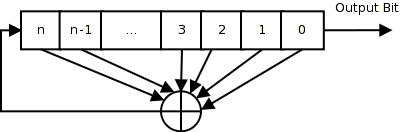
\includegraphics[scale=0.5]{images/lfsr}
    \caption{Linear feedback shift register (Fibonacci configuration)}
    \label{fig:lfsr-fib}
\end{figure}
Another type of LFSR is called a Galois configuration. It has the same
properties, but the feedback scheme is different: each bit in the tap sequence
is XORed with the output bit and replaced; the output bit then becomes the new
left-most bit (figure \ref{fig:lfsr-galois}).
\begin{figure}[htbp]
    \centering
    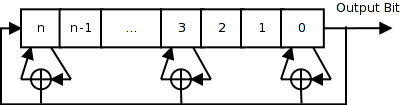
\includegraphics[scale=0.5]{images/lfsr_galois}
    \caption{Linear feedback shift register (Galois configuration)}
    \label{fig:lfsr-galois}
\end{figure}
A sequence generated by LFSR is linear by itself and therefore useless for
cryptography. It is possible to recover the LFSR structure from intercepting
only $2n$ bits of the generator using Berlekamp-Massey algorithm~\cite{joux:algorithmic_cryptanalysis}.

Feedback with carry shift registers (FCSR) are similar to LFSRs but instead of
XORing the tapping sequence bits are added to the carry register. The result
reduced modulo 2 becomes the feedback bit of the register and the result divided
by 2 becomes the new value of the carry register.

The carry register has to be at least $\log_2 t$, where $t$ is the number of
taps. Thus, before the carry register is
filled there are some states of FCSR that never repeat. The maximum period of
FCSR differs from the one of LFSR. It equals to $q - 1$, where $q$ is the
connection integer and defined as
\mbox{$q = 2 q_1 + 2^2 q_2 + 2^4 q_4 + \cdots + 2^n q_n - 1$}; $q$ has to be a prime
for which 2 is a primitive root. In fact not every initial state guarantees
maximum period of the register. That means the all pseudo-random sequence
generators based on FCSR will have a set of weak
keys~\cite{schneier:applied_cryptography:2}.

Non-linear feedback shift registers (NLFSR) use non-linear feedback function.
Such stream ciphers as Grain and Trivium are based on NLFSRs. The idea both
behind NLFSRs and FCSRs is to ensure high non-linearity of the output sequence.
However such non-linear behavior makes the analysis of such registers almost
impossible. The described registers are unpredictable --- they don't guarantee
maximal-period sequence, which also depends on the initial state of the register,
output sequences may have biases of zeroes and ones or contain long bit series.
Hereby, the advantage of these registers may at the same time lead to critical
flaw. Consequently, NLFSRs and FCSRs should be used with utmost caution.


\subsubsection{Clock control}

Clock control is one of several ways to introduce high nonlinearity in
pseudo-random sequence generated by linear feedback shift registers. The rate of
register clocking varies either depending on several LFSRs or on certain bits
of the register state~\cite{usm:streamciphers}. As will be shown further, the combination of clock
control, combination and filter generators allow to form a pseudo-random
sequence satisfying all statistic requirements and yet resistant to known
attacks.

\subsubsection{Generators}

The use of feedback shift registers for cryptographic applications is possible by
combining several registers into a single generator.

The technique of combining outputs of several
registers by a Boolean function is called \textit{combination generator}
(figure~\ref{fig:comb-gen}). The output sequence $s_t$ of a combination generator
composed on $n$ LFSRs is given by
\begin{equation}
    \label{eqn:comb-gen-seq}
    s_t = f(u_1, u_2, \cdots, u_n), \enspace \forall t \leq 0 \enspace,
\end{equation}

where $u_i$ denotes the sequence generated by the $i$-th LFSR and $f$ is a
function of $n$ variables~\cite{encyclopedia_of_cryptography}.
\begin{figure}[htbp]
    \centering
    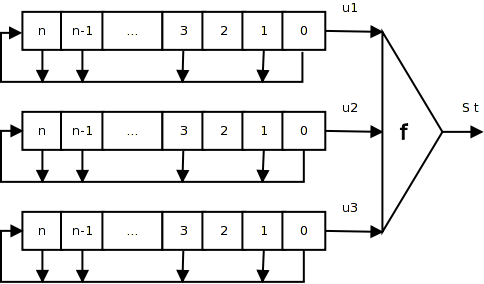
\includegraphics[scale=0.5]{images/comb-gen}
    \caption{Combination generator}
    \label{fig:comb-gen}
\end{figure}
The output of the $f$ function must be uniformly distributed and balanced in
order to produce pseudo-random sequences.

Linear complexity of the keystream generated by a combination generator composed
of $n$ LFSRs with primitive feedback polynomials combined by a Boolean function
$f$ equals to
\begin{equation}
    \label{eqn:lin-complexity}
    f(L_1, L_2, \cdots, L_n) \enspace,
\end{equation}

where the algebraic normal form of $f$ is evaluated over
integers and all lengths $L_1, \cdots, L_n$ are distinct and greater than 2.
High linear complexity of the generator is required to ensure that
Berlekamp-Massey algorithm is computationally infeasible.

Combination generators are vulnerable to correlation attacks based on
recovering the initial states of all LFSRs from the knowledge of some sequence
produced by the generator (known plaintext attack). In order to protect
generators from this kind of attacks, the LFSR feedback polynomials should not
be sparse to ensure a high correlation-immunity order of the combining function.
However the correlation-immunity of a balanced Boolean function of $n$ variables
is limited with $n - 1 - deg(f)$~\cite{encyclopedia_of_cryptography}. Tradeoffs
between high algebraic degree, high nonlinearity and high correlation-immunity
may be outwitted replacing the combining function by a finite state automaton
with memory.

\textit{Filter generators}, in distinction of combination generators, consist of
single LFSR and its state is filtered by a nonlinear
function~(figure~\ref{fig:filter-gen}). The output of the function is a
pseudo-random sequence formed by the generator. Just like in combination
generators the filtering function must be uniformly distributed and balanced.
\begin{figure}[htbp]
    \centering
    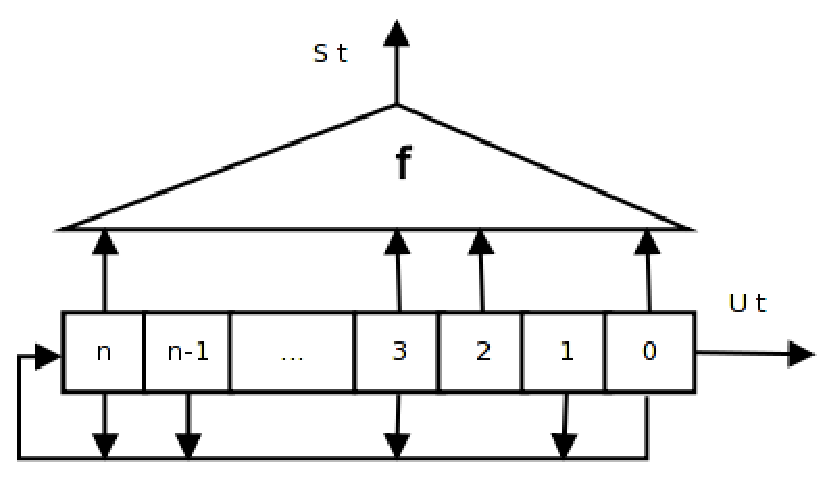
\includegraphics[scale=0.5]{images/filter-gen}
    \caption{Filter generator}
    \label{fig:filter-gen}
\end{figure}

Any filter generator can be represented by a corresponding combination generator
consisting of $n$ copies of the LFSR with shifted initial states when the
combining function complies the filtering function.

Filter generators are vulnerable to fast correlation and generalized inversion
attacks~\cite{canteaut:invattack}. Filtering function should be highly nonlinear
in order to resist the fast correlation attack. The inversion attack depends on
the largest spacing between two taps of the LFSR which conflicts with the
statement that LFSRs should use dense polynomials. Also the greatest common
divisor of all spaces between taps should be equal to 1 or else the inversion
attack could be simplified~\cite{encyclopedia_of_cryptography}.

Algebraic attacks are also applicable to filter generators since a keystream
bit can be represented by a function of $L$ initial bits of the LFSR. Therefore,
knowing $N$ keystream bits allows to form an algebraic system of $N$ equations
of $L$ variables. Usage of Gr\"obner bases (which may be viewed as nonlinear
generalization of Gaussian elimination for linear systems) enables an attacker
to lower the degree of equations until the recovery of LFSR initial state is
possible by solving the algebraic system even with filtering function of high
degree.

Some designs of LFSR-based generators that promise to be secure are considered
further.

\textit{Alternating stop-and-go generator} uses three LFSRs of different length.
LFSR-1 controls clocking of the other two. If output of LFSR-1 is 0, LFSR-3 is
clocked, if its output is 1, LFSR-2 is clocked. The output of the generator is
the XOR of LFSR-2 and LFSR-3.  A correlation attack on LFSR-1 exists, but it
does not threaten the generator's
security~\cite{schneier:applied_cryptography:2}.

\textit{Bilateral stop-and-go generator} uses two LFSRs of length $n$ and its
output bit equals to XOR of the outputs of each LFSR. The functioning of
the generator is described by algorithm~\ref{alg:stop-go-gen}.
\begin{algorithm}
    \caption{Bilateral stop-and-go generator functioning}
    \label{alg:stop-go-gen}

    \SetKw{Land}{and}
    \SetKwData{LfsrI}{LFSR-1}
    \SetKwData{LfsrII}{LFSR-2}
    \SetKwFunction{Output}{Output of}
    \SetKwFunction{Block}{Block}
    \DontPrintSemicolon

    \If{\Output{\LfsrII at time $t-1$} == $0$ \Land \;
    \Indp \Output{\LfsrII at time $t-2$} == $1$ \;}{
    \Block(\LfsrII at time $t$)
    }\;
    \If{\Output{\LfsrI at time $t-1$} == $0$ \Land \;
    \Indp \Output{\LfsrI at time $t-2$} == $1$ \Land \;
    \LfsrI clocked at time $t$ \;}{
    \Block(\LfsrII at time $t$)
    }\;
\end{algorithm}
So far no critical attacks on this generator have been presented. Another
alternative is filter generator that consists in forming cryptographically
strong pseudo-random sequence as some nonlinear function of a state of the
single register~\cite{robshaw:rsa:streamciphers}.

The idea behind the \textit{shrinking generator} is simple and uses two LFSRs.
Both of them are clocked each time: if the output of LFSR-1 is 1, then the
generator outputs bit from LFSR-2, otherwise both bits are discarded and the
LFSRs are clocked again. The generator is said to be secure if no sparse
polynomials are used in LFSRs, but the downside is irregular output rate.
This problem can be solved by buffering though it complicates implementation.

\textit{Self-shrinking generator} is similar to shrinking generator but uses
pairs of bits from a single LFSR. After clocking the register twice output bits
are analysed: if the first bit is 1, the output is the second bit; if the first
bit is 0, bits are discarded and the register is clocked again. This generator
is slower but requires less memory. However its properties are hard to analyse.

\subsubsection{T-functions}

A new building block for symmetric ciphers called T-function was introduced by
Klimov and Shamir in 2003~\cite{klimov:tfunc}. T-function is a class of
invertible mappings that mix arithmetic and boolean operations and process
full machine words.

Consider a construction where each input variable has $n$ bits, and $m$ input
variables are placed in $m$ rows of \mbox{$m \times n$ bit} matrix. Than a
T-function is defined by mapping
\begin{equation}
    \label{eqn:t-func}
    f: \mathbb{B}^{m \times n} \rightarrow \mathbb{B}^{k \times n} \enspace,
\end{equation}%

where $\mathbb{B} = \{0, 1\}$ and each $k$-th column of the output depends only on
the first $k$ columns of the input. In general, in order to compute the $k$-th
output bit only input bits $0, 1, \cdots, k$ must be known. Most machine
instructions are T-functions: negation, addition, subtraction, multiplication, left
shift, which is identical to multiplication by $2$. Any combination of
T-functions is also a T-function.

The name of such transformation refers to the triangular dependence of the following
form~\cite{dblp:conf/fse/klimovs05}:
\begin{equation}
    \left(
    \begin{array}{c}
        \left[ f(x) \right]_0 \\
        \left[ f(x) \right]_1 \\
        \left[ f(x) \right]_2 \\
        \vdots \\
        \left[ f(x) \right]_{n-1} \\
    \end{array} \right)%
    = \left(
    \begin{array}{c}
        f_0([x]_0) \\
        f_1([x]_0, [x]_1) \\
        f_2([x]_0, [x]_1, [x]_2) \\
        \vdots \\
        f_{n-1}([x]_0, \cdots, [x]_{n-2}, [x]_{n-1})
    \end{array} \right) \enspace,
\end{equation}

where $\left[ f(x) \right]_k$ is the $k$-th output column and
$[x]k-1, \cdots, [x]_0$ --- first $k$ input columns.

The primary advantage of T-functions is computation efficiency both in hardware
and software implementation on modern processors. Despite of having desirable
cryptographic properties, some functions revealed weaknesses to correlation,
algebraic and distinguishing attacks~\cite{mycrypt/kunzli_jm05} with a complexity of
$2^{32}$. Even though usage of T-functions is highly attractive, reasonable
security of such transformations should be proved first.


\section{Formulation of the problem}

In spite of advances in mathematic methods of modern cryptography, real world
security system often end up using vulnerable ciphers due to insufficient
preliminary analysis. By the time the security cryptoalgorithm is properly
studied, the cipher itself is already deployed in global system -- switching is
expensive and hard technologically.

In order to prevent such situations methods for efficient cryptographic security
analysis of ciphers need to be propagated and best practices for cryptographic
primitives design and evaluation provided. Most widely used cryptanalytic
methods (linear and differential cryptanalysis, etc.) are based on statistical
approach and require tremendous amount of data for sane evaluation. Even with
exponential growth of computational power it most probably will be impossible
neither in the near future nor any given time in future to apply these
statistical methods to modern full-scale ciphers.

To make statistical cryptanalytic methods somewhat applicable to ciphers used in
modern security systems the concept of baby-ciphers has been introduced. The
concept implied proportional shrinking of all transformations of the cipher in
order to get a baby-version -- still similar to the original cipher but its full
statistical analysis is computationally feasible. However the correspondence of
such statistical evaluation to the full-scale original cipher hasn't yet been
proved.

Nonetheless algebraic analysis of cryptoalgorithms and recent advances in
computational algebra allow to obtain systems of multivariate equations that
mathematically describe the behaviour of full-scale ciphers and require only few
pairs of \mbox{plaintext/ciphertext} for valid analysis. Most equations systems
for modern ciphers are still hard to compute, but the complexity gap for solving
full-scale system of equations is times smaller than for statistical methods to
analyze full-scale cipher.

Though the algebraic analysis method is promising, it is not yet widely used and
has been applied to only few ciphers. In order to perform algebraic analysis of
any cryptoalgorithm it first must be defined by a system of multivariate
non-linear equations. Therefore to make the algebraic cryptanalysis technique
commonly used by cryptologists some patterns and best practices in constructing
polynomial equations for modern ciphers must be made available to the public.
Not only the theoretical part is important for valid evaluation. The ready to
use reference software implementation with examples is the key wide
applicability of algebraic analysis methods.

In order to solve the described issues and enable aglebraic analysis efficiently
applicable for modern symmetric cipher following solutions need to be provided:

\begin{enumerate}
    \item develop guide lines for constructing system of non-linear equations for
modern ciphers as well as for individual transformations commonly used in modern
ciphers;
    \item describe the most efficient methods and provide best practices for
        solving algebraic equations systems;
    \item use provided methods for applying algebraic attack to actual ciphers;
    \item describe needed software tools and provide reference implementation
        for all steps of algebraic attack for easy reproduce and application to
        other ciphers.
\end{enumerate}




% AUTHOR: Ruslan Kiianchuk <ruslan.kiianchuk@gmail.com>


\chapter{Algebraic analysis of symmetric block ciphers}
\label{sec:algebraic}

Being a fairly new technique, algebraic cryptanalysis is one of the most
promissory and powerful methods for analysing cryptographic
algorithms~\cite{Albrecht2010}. It implies modeling a cryptographic algorithm
by a set of algebraic equations that form multivariate polynomial equations
system over finite field. The lower degree such system has the easier it is to
solve, so it is a rule of thumb in algebraic analysis to construct algebraic
systems that contain only quadratic multivariate 
(MQ\footnote{It also became a widespread practice to denote the problem of
solving multivariate quadratic equation systems as MQ for short.}) 
equations.

The essence of algebraic cryptanalysis is an assumption made by Claude Shannon
in~\cite{shannon:secrecy} that binds cipher security to the difficulty of
solving the corresponding algebraic equations set:
``Breaking a good cipher should require as much work as solving a system of
simultaneous equations in a large number of unknowns of a complex
type''.

The main advantage of algebraic cryptanalysis over other methods is the need
for only few pairs of plaintexts and ciphertexts. Breaking Keeloq cipher is
a good example of successful algebraic attack on full scale
cryptoalgorithm~\cite{bard2009algebraic}. The attack allows to recover the
encryption key in $2^{14.77}$ times faster than a brute force search.

An Advanced Encryption Standard (AES) that is also widely used outside of the
USA is potentially vulnerable to XSL attack (a type of algebraic cryptanalysis).
The attack is claimed to significantly weaken the cipher. Even though the
practical applicability of the attack hasn't yet been proven, the algebraic 
structure of AES that is efficiently described with algebraic equations system
may be compliant to such analysis as mentioned in~\cite{ferguson2003practical}: 

``We have one criticism of AES: we don't quite trust the security. What concerns
us the most about AES is its simple algebraic structure. No other block cipher
we know of has such a simple algebraic representation. We have no idea whether
this leads to an attack or not, but not knowing is reason enough to be skeptical
about the use of AES.'' \textit{(Bruce Schneier, Niels Ferguson)}.

Given an equations system that completely describes the cryptographic algorithm
one gets a powerful tool for researching its hidden properties. However such
systems are hard to solve for full scale ciphers. Complexity of polynomial
systems is usually described by the number of equations, their degree and number
of variables they have~\cite{bard2009algebraic}. 

It is shown in~\cite{Courtois:MQ-NPhard} that solving multivariate quadratic
equations systems over $GF(2)$ (MQ) and finding satisfying solutions for boolean
expressions in several variables (SAT) are NP-hard problems. But their
complexity significantly drops if the system becomes overdefined, i.\,e. there
are much more equations than unknowns~\cite{DBLP:conf/asiacrypt/CourtoisP02}.


\section{Construction of algebraic equations for cryptographic primitives}
\label{sec:equations}

Generally an algebraic attack is executed in two steps:
\begin{enumerate}
    \item An analyzed cipher is described by multivariate equations system;
    \item For given plaintext and ciphertext pairs the equation is solved for
        recovering the key bits.
\end{enumerate}
Therefore to complete the first step, every transformation of the cipher has to
be defined by polynomial equations. If all input variables are replaced by given
bits and the rest of variables obtain output and intermediate values equal to
those of original transformation, then the equations are correct.

Most of cryptographic algorithms consist of the following operations:
\begin{itemize}
    \item bit permutations;
    \item modular addition (XOR is equivalent to modulo 2 addition);
    \item logical operations (AND, OR, Negation);
    \item substitution (S-boxes);
\end{itemize}

As will be shown further, these transformations may be completely defined by
polynomial equations systems in algebraic normal form (ANF), that is expressed
using operations \textit{Exclusive Or} (XOR) and \textit{conjunction} (logical
AND).

\subsection{Logical operations}

Algebraic normal form consists of two operations: AND, XOR, so these are trivial
to describe. Negation may be expressed by applying XOR with constant~$1$.
Logical OR operation may be expressed in ANF as follows:
\begin{equation}
x \lor y = (x \land y) \oplus x \oplus y\enspace.
\end{equation}
Correctness of the proposed equation may by verified by constructing a truth
table for both expressions (figure~\ref{fig:eq_logic_or}).
\begin{figure}[htbp]
    \begin{subfigure}[b]{0.5\textwidth}
        \centering
        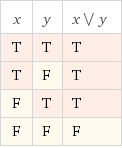
\includegraphics[scale=0.7]{images/eq_logic_or}
        \caption{Logical OR in CNF}
    \end{subfigure}
    \quad
    \begin{subfigure}[b]{0.5\textwidth}
        \centering
        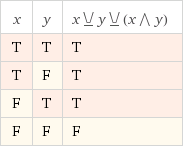
\includegraphics[scale=0.7]{images/eq_logic_or_anf}
        \caption{Logical OR in ANF}
    \end{subfigure}
	\caption{Truth tables for logical OR}
	\label{fig:eq_logic_or}
\end{figure}


\subsection{Bit permutations}

Consider simple $4$-bit permutation that needs to be defined by equations
system (figure~\ref{fig:eq_permutation}). After matching each bit to certain
variable one could obtain the corresponding equations system.
\begin{equation}
\label{eqn:eq_permutation_expl}
\left\{
	\begin{array}{ll}
        y_0 = x_3; \\
        y_1 = x_2; \\
        y_2 = x_1; \\
        y_3 = x_0. \\
	\end{array} \right.
\end{equation}
Then equations (\ref{eqn:eq_permutation_expl}) could be transformed to implicit
form to obtain the final polynomials:
\begin{equation}
\label{eqn:eq_permutation_impl}
\left\{
	\begin{array}{ll}
        y_0 \oplus x_3 = 0; \\
        y_1 \oplus x_2 = 0; \\
        y_2 \oplus x_1 = 0; \\
        y_3 \oplus x_0 = 0. \\
	\end{array} \right.
\end{equation}
So the given $4$-bit permutation has been defined by $4$ equations in $8$
variables.  Such solution is simple but unfortunately introduces more variables
than equations which may lead to underdefined and therefore unsolvable system.
However more efficient approach exists. Since there is no multiplication in this
transformation that could increase equations degree and the variables are only
renamed, they may be just reordered for the following transformation to receive
correct values. That way no additional equations or variables are introduced at
all.

Any cyclic bit shift is just a special case of ordered permutation and is
defined similarly.

\begin{figure}[htbp]
	\centering
    % Graphic for TeX using PGF
% Title: /home/zoresvit/devel/texmf/dstu-3008-95/images/eq_permutation.dia
% Creator: Dia v0.97.2
% CreationDate: Mon Jun  3 02:38:01 2013
% For: zoresvit
% \usepackage{tikz}
% The following commands are not supported in PSTricks at present
% We define them conditionally, so when they are implemented,
% this pgf file will use them.
\ifx\du\undefined
  \newlength{\du}
\fi
\setlength{\du}{15\unitlength}
\begin{tikzpicture}
\pgftransformxscale{1.000000}
\pgftransformyscale{-1.000000}
\definecolor{dialinecolor}{rgb}{0.000000, 0.000000, 0.000000}
\pgfsetstrokecolor{dialinecolor}
\definecolor{dialinecolor}{rgb}{1.000000, 1.000000, 1.000000}
\pgfsetfillcolor{dialinecolor}
\pgfsetlinewidth{0.100000\du}
\pgfsetdash{}{0pt}
\pgfsetdash{}{0pt}
\pgfsetbuttcap
{
\definecolor{dialinecolor}{rgb}{0.000000, 0.000000, 0.000000}
\pgfsetfillcolor{dialinecolor}
% was here!!!
\definecolor{dialinecolor}{rgb}{0.000000, 0.000000, 0.000000}
\pgfsetstrokecolor{dialinecolor}
\draw (19.000000\du,5.000000\du)--(19.000000\du,6.000000\du);
}
\pgfsetlinewidth{0.100000\du}
\pgfsetdash{}{0pt}
\pgfsetdash{}{0pt}
\pgfsetbuttcap
{
\definecolor{dialinecolor}{rgb}{0.000000, 0.000000, 0.000000}
\pgfsetfillcolor{dialinecolor}
% was here!!!
\definecolor{dialinecolor}{rgb}{0.000000, 0.000000, 0.000000}
\pgfsetstrokecolor{dialinecolor}
\draw (24.000000\du,5.000000\du)--(24.000000\du,6.000000\du);
}
\pgfsetlinewidth{0.100000\du}
\pgfsetdash{}{0pt}
\pgfsetdash{}{0pt}
\pgfsetbuttcap
{
\definecolor{dialinecolor}{rgb}{0.000000, 0.000000, 0.000000}
\pgfsetfillcolor{dialinecolor}
% was here!!!
\definecolor{dialinecolor}{rgb}{0.000000, 0.000000, 0.000000}
\pgfsetstrokecolor{dialinecolor}
\draw (21.500000\du,5.000000\du)--(21.500000\du,6.000000\du);
}
\pgfsetlinewidth{0.100000\du}
\pgfsetdash{}{0pt}
\pgfsetdash{}{0pt}
\pgfsetbuttcap
{
\definecolor{dialinecolor}{rgb}{0.000000, 0.000000, 0.000000}
\pgfsetfillcolor{dialinecolor}
% was here!!!
\definecolor{dialinecolor}{rgb}{0.000000, 0.000000, 0.000000}
\pgfsetstrokecolor{dialinecolor}
\draw (26.500000\du,5.000000\du)--(26.500000\du,6.000000\du);
}
\pgfsetlinewidth{0.100000\du}
\pgfsetdash{}{0pt}
\pgfsetdash{}{0pt}
\pgfsetbuttcap
{
\definecolor{dialinecolor}{rgb}{0.000000, 0.000000, 0.000000}
\pgfsetfillcolor{dialinecolor}
% was here!!!
\definecolor{dialinecolor}{rgb}{0.000000, 0.000000, 0.000000}
\pgfsetstrokecolor{dialinecolor}
\draw (19.000000\du,10.000000\du)--(19.000000\du,11.000000\du);
}
\pgfsetlinewidth{0.100000\du}
\pgfsetdash{}{0pt}
\pgfsetdash{}{0pt}
\pgfsetbuttcap
{
\definecolor{dialinecolor}{rgb}{0.000000, 0.000000, 0.000000}
\pgfsetfillcolor{dialinecolor}
% was here!!!
\definecolor{dialinecolor}{rgb}{0.000000, 0.000000, 0.000000}
\pgfsetstrokecolor{dialinecolor}
\draw (24.000000\du,10.000000\du)--(24.000000\du,11.000000\du);
}
\pgfsetlinewidth{0.100000\du}
\pgfsetdash{}{0pt}
\pgfsetdash{}{0pt}
\pgfsetbuttcap
{
\definecolor{dialinecolor}{rgb}{0.000000, 0.000000, 0.000000}
\pgfsetfillcolor{dialinecolor}
% was here!!!
\definecolor{dialinecolor}{rgb}{0.000000, 0.000000, 0.000000}
\pgfsetstrokecolor{dialinecolor}
\draw (21.500000\du,10.000000\du)--(21.500000\du,11.000000\du);
}
\pgfsetlinewidth{0.100000\du}
\pgfsetdash{}{0pt}
\pgfsetdash{}{0pt}
\pgfsetbuttcap
{
\definecolor{dialinecolor}{rgb}{0.000000, 0.000000, 0.000000}
\pgfsetfillcolor{dialinecolor}
% was here!!!
\definecolor{dialinecolor}{rgb}{0.000000, 0.000000, 0.000000}
\pgfsetstrokecolor{dialinecolor}
\draw (26.500000\du,10.000000\du)--(26.500000\du,11.000000\du);
}
\pgfsetlinewidth{0.100000\du}
\pgfsetdash{}{0pt}
\pgfsetdash{}{0pt}
\pgfsetbuttcap
{
\definecolor{dialinecolor}{rgb}{0.000000, 0.000000, 0.000000}
\pgfsetfillcolor{dialinecolor}
% was here!!!
\definecolor{dialinecolor}{rgb}{0.000000, 0.000000, 0.000000}
\pgfsetstrokecolor{dialinecolor}
\draw (19.000000\du,6.000000\du)--(26.500000\du,10.000000\du);
}
\pgfsetlinewidth{0.100000\du}
\pgfsetdash{}{0pt}
\pgfsetdash{}{0pt}
\pgfsetbuttcap
{
\definecolor{dialinecolor}{rgb}{0.000000, 0.000000, 0.000000}
\pgfsetfillcolor{dialinecolor}
% was here!!!
\definecolor{dialinecolor}{rgb}{0.000000, 0.000000, 0.000000}
\pgfsetstrokecolor{dialinecolor}
\draw (21.500000\du,6.000000\du)--(24.000000\du,10.000000\du);
}
\pgfsetlinewidth{0.100000\du}
\pgfsetdash{}{0pt}
\pgfsetdash{}{0pt}
\pgfsetbuttcap
{
\definecolor{dialinecolor}{rgb}{0.000000, 0.000000, 0.000000}
\pgfsetfillcolor{dialinecolor}
% was here!!!
\definecolor{dialinecolor}{rgb}{0.000000, 0.000000, 0.000000}
\pgfsetstrokecolor{dialinecolor}
\draw (24.000000\du,6.000000\du)--(21.500000\du,10.000000\du);
}
\pgfsetlinewidth{0.100000\du}
\pgfsetdash{}{0pt}
\pgfsetdash{}{0pt}
\pgfsetbuttcap
{
\definecolor{dialinecolor}{rgb}{0.000000, 0.000000, 0.000000}
\pgfsetfillcolor{dialinecolor}
% was here!!!
\definecolor{dialinecolor}{rgb}{0.000000, 0.000000, 0.000000}
\pgfsetstrokecolor{dialinecolor}
\draw (26.500000\du,6.000000\du)--(19.000000\du,10.000000\du);
}
% setfont left to latex
\definecolor{dialinecolor}{rgb}{0.000000, 0.000000, 0.000000}
\pgfsetstrokecolor{dialinecolor}
\node[anchor=west] at (18.000000\du,4.500000\du){$x_0$};
% setfont left to latex
\definecolor{dialinecolor}{rgb}{0.000000, 0.000000, 0.000000}
\pgfsetstrokecolor{dialinecolor}
\node[anchor=west] at (20.500000\du,4.500000\du){$x_1$};
% setfont left to latex
\definecolor{dialinecolor}{rgb}{0.000000, 0.000000, 0.000000}
\pgfsetstrokecolor{dialinecolor}
\node[anchor=west] at (23.000000\du,4.500000\du){$x_2$};
% setfont left to latex
\definecolor{dialinecolor}{rgb}{0.000000, 0.000000, 0.000000}
\pgfsetstrokecolor{dialinecolor}
\node[anchor=west] at (26.000000\du,4.500000\du){$x_3$};
% setfont left to latex
\definecolor{dialinecolor}{rgb}{0.000000, 0.000000, 0.000000}
\pgfsetstrokecolor{dialinecolor}
\node[anchor=west] at (18.000000\du,12.000000\du){$y_0$};
% setfont left to latex
\definecolor{dialinecolor}{rgb}{0.000000, 0.000000, 0.000000}
\pgfsetstrokecolor{dialinecolor}
\node[anchor=west] at (20.500000\du,12.000000\du){$y_1$};
% setfont left to latex
\definecolor{dialinecolor}{rgb}{0.000000, 0.000000, 0.000000}
\pgfsetstrokecolor{dialinecolor}
\node[anchor=west] at (23.000000\du,12.000000\du){$y_2$};
% setfont left to latex
\definecolor{dialinecolor}{rgb}{0.000000, 0.000000, 0.000000}
\pgfsetstrokecolor{dialinecolor}
\node[anchor=west] at (26.000000\du,12.000000\du){$y_3$};
\end{tikzpicture}

	\caption{$4$-bit permutation}
	\label{fig:eq_permutation}
\end{figure}

\subsection{Modular addition}
\label{seq:key-add-eqn}

During the Ukrainian national public cryptographic competition the following
method for defining modular addition with equations system has been proposed 
by the author of \textit{Labyrinth} block cipher.

Modular addition $R = X + Y$ of two $n$-bit numbers is defined as 
\begin{equation}
\label{eqn:add}
X = (x_0, \hdots, x_{n-1}), \; 
Y = (y_0, \hdots, y_{n-1}), \;
R = (r_0, \hdots, r_{n-1}),
\end{equation}

where $i$ --- is a bit number, so $x_i$ represents $i$-th bit of number $X$. 
Then the addition on a bit level is defined as follows:
\begin{equation}
\label{eqn:trivial-mod-add}
r_i = x_i \oplus y_i \oplus c_{i-1} \enspace,
\end{equation}

where $c_i$ is a carry bit variable and is defined by \eqref{eqn:carry-bit}.
\begin{equation}
\label{eqn:carry-bit}
c_i = r_{i+1} \oplus x_{i+1} \oplus y_{i+1} \enspace.
\end{equation}
The goal is to get null space equations for every addition bit without
explicitly using the carry variable. It turns out that for addition bits 
$0 < i < (n - 1)$ three implicit equations may be defined:
\begin{equation}
\label{eqn:add-with-carry}
\left\{
	\begin{array}{ll}
        (x_i \oplus r_i) (x_i \oplus c_i) = 0; \\
        (y_i \oplus r_i) (y_i \oplus c_i) = 0; \\
        (x_i \oplus y_i) \cdot r_i \oplus x_i y_i \oplus x_i \oplus y_i \oplus c_i = 0.
	\end{array} \right.
\end{equation}
The final equation system that defines every addition bit may be extracted
from~\eqref{eqn:add-with-carry} by substituting every $c_i$ variable according
to~\ref{eqn:carry-bit}:
\begin{equation}
\label{eqn:mod-add}
\left\{
	\begin{array}{ll}
        x_i \oplus x_i r_i \oplus x_i r_{i+1} \oplus x_i x_{i+1} \oplus x_i y_{i+1} \oplus r_i r_{i+1} \oplus r_i x_{i+1} \oplus r_i y_{i+1} = 0; \\
        y_i \oplus y_i r_i \oplus y_i r_{i+1} \oplus y_i x_{i+1} \oplus y_i y_{i+1} \oplus r_i r_{i+1} \oplus r_i x_{i+1} \oplus r_i y_{i+1} = 0; \\
        x_i r_i \oplus y_i r_i \oplus x_i y_i \oplus x_i \oplus y_i \oplus r_{i+1} \oplus x_{i+1} \oplus y_{i+1} = 0.
	\end{array} \right.
\end{equation}
Thereby a single addition bit is defined by three equations of degree 2 each
containing $12$ quadratic terms. Even though the equations in
\eqref{eqn:mod-add} fully describe $n$-bit modular addition, adding a
redundant equation $r_0 = x_0 + y_0$ for the very first bit was found to give
crucial increase on system solving performance.


\subsection{S-boxes}

An arbitrary S-box is fully defined by equations of degree 2 that can be
obtained by finding null space equations as described in~\cite{kleiman:xsl}.

Consider the S-box $(7, 6, 0, 4, 2, 5, 1, 3)$ for example. To find 
corresponding null space equations the following matrix $8 \times 22$ is
constructed.  Each row contains the values of all possible $22$ monomials for
each of $8$ possible inputs for variables $\{x_0, x_1, x_2, x_3\}$.
\begin{equation}
    \label{eqn:sbox-matr}
    \left(
    \begin{array}{lllllllll}
        1 &\quad 1 &\quad 1 &\quad 1 &\quad 1 &\quad 1 &\quad 1 &\quad 1 &\quad 1       \\[-1ex]
        0 &\quad 0 &\quad 0 &\quad 0 &\quad 1 &\quad 1 &\quad 1 &\quad 1 &\quad x_0     \\[-1ex]
        0 &\quad 0 &\quad 1 &\quad 1 &\quad 0 &\quad 0 &\quad 1 &\quad 1 &\quad x_1     \\[-1ex]
        0 &\quad 1 &\quad 0 &\quad 1 &\quad 0 &\quad 1 &\quad 0 &\quad 1 &\quad x_2     \\[-1ex]
        1 &\quad 1 &\quad 0 &\quad 1 &\quad 0 &\quad 1 &\quad 0 &\quad 0 &\quad y_0     \\[-1ex]
        1 &\quad 1 &\quad 0 &\quad 0 &\quad 1 &\quad 0 &\quad 0 &\quad 1 &\quad y_1     \\[-1ex]
        1 &\quad 0 &\quad 0 &\quad 0 &\quad 0 &\quad 1 &\quad 1 &\quad 1 &\quad y_2     \\[-1ex]
        0 &\quad 0 &\quad 0 &\quad 0 &\quad 0 &\quad 0 &\quad 1 &\quad 1 &\quad x_0 x_1 \\[-1ex]
        0 &\quad 0 &\quad 0 &\quad 0 &\quad 0 &\quad 1 &\quad 0 &\quad 1 &\quad x_0 x_2 \\[-1ex]
        0 &\quad 0 &\quad 0 &\quad 0 &\quad 0 &\quad 1 &\quad 0 &\quad 0 &\quad x_0 y_0 \\[-1ex]
        0 &\quad 0 &\quad 0 &\quad 0 &\quad 1 &\quad 0 &\quad 0 &\quad 1 &\quad x_0 y_1 \\[-1ex]
        0 &\quad 0 &\quad 0 &\quad 0 &\quad 0 &\quad 1 &\quad 1 &\quad 1 &\quad x_0 y_2 \\[-1ex]
        0 &\quad 0 &\quad 0 &\quad 1 &\quad 0 &\quad 0 &\quad 0 &\quad 1 &\quad x_1 x_2 \\[-1ex]
        0 &\quad 0 &\quad 0 &\quad 1 &\quad 0 &\quad 0 &\quad 0 &\quad 0 &\quad x_1 y_0 \\[-1ex]
        0 &\quad 0 &\quad 0 &\quad 0 &\quad 0 &\quad 0 &\quad 0 &\quad 1 &\quad x_1 y_1 \\[-1ex]
        0 &\quad 0 &\quad 0 &\quad 0 &\quad 0 &\quad 0 &\quad 1 &\quad 1 &\quad x_1 y_2 \\[-1ex]
        0 &\quad 1 &\quad 0 &\quad 1 &\quad 0 &\quad 1 &\quad 0 &\quad 0 &\quad x_2 y_0 \\[-1ex]
        0 &\quad 1 &\quad 0 &\quad 0 &\quad 0 &\quad 0 &\quad 0 &\quad 1 &\quad x_2 y_1 \\[-1ex]
        0 &\quad 0 &\quad 0 &\quad 0 &\quad 0 &\quad 1 &\quad 0 &\quad 1 &\quad x_2 y_2 \\[-1ex]
        1 &\quad 1 &\quad 0 &\quad 0 &\quad 0 &\quad 0 &\quad 0 &\quad 0 &\quad y_0 y_1 \\[-1ex]
        1 &\quad 0 &\quad 0 &\quad 0 &\quad 0 &\quad 1 &\quad 0 &\quad 0 &\quad y_0 y_2 \\[-1ex]
        1 &\quad 0 &\quad 0 &\quad 0 &\quad 0 &\quad 0 &\quad 0 &\quad 1 &\quad y_1 y_2
    \end{array} \right)
\end{equation}
The null space equations are then obtained by applying Gaussian elimination to
the matrix.

\begin{equation}
    \label{eqn:sbox-equations}
    \left(
    \begin{array}{llllllllr}
        1 & 0 & 0 & 0 & 0 & 0 & 0 & 0 & x_0 y_0+ x_1+ x_2+ y_0+ y_1+ 1              \\
        0 & 1 & 0 & 0 & 0 & 0 & 0 & 0 & x_0 y_0+ x_0+ x_1+ y_2+ 1                   \\
        0 & 0 & 1 & 0 & 0 & 0 & 0 & 0 & x_0 y_0+ x_0+ y_0+ 1                        \\
        0 & 0 & 0 & 1 & 0 & 0 & 0 & 0 & x_0 y_0+ x_0+ x_2+ y_1+ y_2                 \\
        0 & 0 & 0 & 0 & 1 & 0 & 0 & 0 & x_0 y_0+ x_0+ x_1+ x_2+ y_0+ y_1+ y_2+ 1    \\
        0 & 0 & 0 & 0 & 0 & 1 & 0 & 0 & x_0 y_0                                     \\
        0 & 0 & 0 & 0 & 0 & 0 & 1 & 0 & x_0 y_0+ x_2+ y_0+ y_2                      \\
        0 & 0 & 0 & 0 & 0 & 0 & 0 & 1 & x_0 y_0+ x_1+ y_1+ 1                        \\
        0 & 0 & 0 & 0 & 0 & 0 & 0 & 0 & x_0 x_2+ x_1+ y_1+ 1                        \\
        0 & 0 & 0 & 0 & 0 & 0 & 0 & 0 & x_0 x_1+ x_1+ x_2+ y_0+ y_1+ y_2+ 1         \\
        0 & 0 & 0 & 0 & 0 & 0 & 0 & 0 & x_0 y_1+ x_0+ x_2+ y_0+ y_2                 \\
        0 & 0 & 0 & 0 & 0 & 0 & 0 & 0 & x_0 y_0+ x_0y_2+ x_1+ x_2+ y_0+ y_1+ y_2+ 1 \\
        0 & 0 & 0 & 0 & 0 & 0 & 0 & 0 & x_1 x_2+ x_0+ x_1+ x_2+ y_2+ 1              \\
        0 & 0 & 0 & 0 & 0 & 0 & 0 & 0 & x_0 y_0+ x_1y_0+ x_0+ x_2+ y_1+ y_2         \\
        0 & 0 & 0 & 0 & 0 & 0 & 0 & 0 & x_0 y_0+ x_1y_1+ x_1+ y_1+ 1                \\
        0 & 0 & 0 & 0 & 0 & 0 & 0 & 0 & x_1 y_2+ x_1+ x_2+ y_0+ y_1+ y_2+ 1         \\
        0 & 0 & 0 & 0 & 0 & 0 & 0 & 0 & x_0 y_0+ x_2y_0+ x_1+ x_2+ y_1+ 1           \\
        0 & 0 & 0 & 0 & 0 & 0 & 0 & 0 & x_2 y_1+ x_0+ y_1+ y_2                      \\
        0 & 0 & 0 & 0 & 0 & 0 & 0 & 0 & x_2 y_2+ x_1+ y_1+ 1                        \\
        0 & 0 & 0 & 0 & 0 & 0 & 0 & 0 & y_0 y_1+ x_0+ x_2+ y_0+ y_1+ y_2            \\
        0 & 0 & 0 & 0 & 0 & 0 & 0 & 0 & y_0 y_2+ x_1+ x_2+ y_0+ y_1+ 1              \\
        0 & 0 & 0 & 0 & 0 & 0 & 0 & 0 & y_1 y_2+ x_2+ y_0                            
    \end{array} \right)
\end{equation}
This yields to $14$ equations that fully describe the S-box transformations.  

\subsection{Feistel network}

Using the described methods of constructing algebraic equations for widely used
cryptographic transformations it is straightforward to define generic Feistel
network with polynomial equations system.

Consider a Feistel network on figure~\ref{fig:eq_feistel}. 
\begin{figure}[htbp]
	\centering
    % Graphic for TeX using PGF
% Title: /home/zoresvit/devel/texmf/dstu-3008-95/images/feistel.dia
% Creator: Dia v0.97.2
% CreationDate: Tue Jun  4 00:25:14 2013
% For: zoresvit
% \usepackage{tikz}
% The following commands are not supported in PSTricks at present
% We define them conditionally, so when they are implemented,
% this pgf file will use them.
\ifx\du\undefined
  \newlength{\du}
\fi
\setlength{\du}{15\unitlength}
\begin{tikzpicture}
\pgftransformxscale{1.000000}
\pgftransformyscale{-1.000000}
\definecolor{dialinecolor}{rgb}{0.000000, 0.000000, 0.000000}
\pgfsetstrokecolor{dialinecolor}
\definecolor{dialinecolor}{rgb}{1.000000, 1.000000, 1.000000}
\pgfsetfillcolor{dialinecolor}
\definecolor{dialinecolor}{rgb}{1.000000, 1.000000, 1.000000}
\pgfsetfillcolor{dialinecolor}
\fill (16.000000\du,2.000000\du)--(16.000000\du,3.900000\du)--(28.000000\du,3.900000\du)--(28.000000\du,2.000000\du)--cycle;
\pgfsetlinewidth{0.100000\du}
\pgfsetdash{}{0pt}
\pgfsetdash{}{0pt}
\pgfsetmiterjoin
\definecolor{dialinecolor}{rgb}{0.000000, 0.000000, 0.000000}
\pgfsetstrokecolor{dialinecolor}
\draw (16.000000\du,2.000000\du)--(16.000000\du,3.900000\du)--(28.000000\du,3.900000\du)--(28.000000\du,2.000000\du)--cycle;
% setfont left to latex
\definecolor{dialinecolor}{rgb}{0.000000, 0.000000, 0.000000}
\pgfsetstrokecolor{dialinecolor}
\node at (22.000000\du,3.145000\du){INPUT};
\definecolor{dialinecolor}{rgb}{1.000000, 1.000000, 1.000000}
\pgfsetfillcolor{dialinecolor}
\fill (16.000000\du,12.000000\du)--(16.000000\du,13.900000\du)--(28.000000\du,13.900000\du)--(28.000000\du,12.000000\du)--cycle;
\pgfsetlinewidth{0.100000\du}
\pgfsetdash{}{0pt}
\pgfsetdash{}{0pt}
\pgfsetmiterjoin
\definecolor{dialinecolor}{rgb}{0.000000, 0.000000, 0.000000}
\pgfsetstrokecolor{dialinecolor}
\draw (16.000000\du,12.000000\du)--(16.000000\du,13.900000\du)--(28.000000\du,13.900000\du)--(28.000000\du,12.000000\du)--cycle;
% setfont left to latex
\definecolor{dialinecolor}{rgb}{0.000000, 0.000000, 0.000000}
\pgfsetstrokecolor{dialinecolor}
\node at (22.000000\du,13.145000\du){OUTPUT};
\definecolor{dialinecolor}{rgb}{1.000000, 1.000000, 1.000000}
\pgfsetfillcolor{dialinecolor}
\fill (30.000000\du,2.000000\du)--(30.000000\du,3.900000\du)--(36.000000\du,3.900000\du)--(36.000000\du,2.000000\du)--cycle;
\pgfsetlinewidth{0.100000\du}
\pgfsetdash{}{0pt}
\pgfsetdash{}{0pt}
\pgfsetmiterjoin
\definecolor{dialinecolor}{rgb}{0.000000, 0.000000, 0.000000}
\pgfsetstrokecolor{dialinecolor}
\draw (30.000000\du,2.000000\du)--(30.000000\du,3.900000\du)--(36.000000\du,3.900000\du)--(36.000000\du,2.000000\du)--cycle;
% setfont left to latex
\definecolor{dialinecolor}{rgb}{0.000000, 0.000000, 0.000000}
\pgfsetstrokecolor{dialinecolor}
\node at (33.000000\du,3.145000\du){SUBKEY};
\pgfsetlinewidth{0.100000\du}
\pgfsetdash{}{0pt}
\pgfsetdash{}{0pt}
\pgfsetbuttcap
{
\definecolor{dialinecolor}{rgb}{0.000000, 0.000000, 0.000000}
\pgfsetfillcolor{dialinecolor}
% was here!!!
\definecolor{dialinecolor}{rgb}{0.000000, 0.000000, 0.000000}
\pgfsetstrokecolor{dialinecolor}
\draw (26.500000\du,4.500000\du)--(26.500000\du,8.000000\du);
}
\pgfsetlinewidth{0.100000\du}
\pgfsetdash{}{0pt}
\pgfsetdash{}{0pt}
\pgfsetmiterjoin
\pgfsetbuttcap
{
\definecolor{dialinecolor}{rgb}{0.000000, 0.000000, 0.000000}
\pgfsetfillcolor{dialinecolor}
% was here!!!
{\pgfsetcornersarced{\pgfpoint{0.000000\du}{0.000000\du}}\definecolor{dialinecolor}{rgb}{0.000000, 0.000000, 0.000000}
\pgfsetstrokecolor{dialinecolor}
\draw (33.000000\du,3.900000\du)--(33.000000\du,5.264262\du)--(26.773042\du,5.264262\du)--(26.773042\du,5.269734\du);
}}
% setfont left to latex
\definecolor{dialinecolor}{rgb}{0.000000, 0.000000, 0.000000}
\pgfsetstrokecolor{dialinecolor}
\node[anchor=west] at (16.000000\du,1.500000\du){0};
% setfont left to latex
\definecolor{dialinecolor}{rgb}{0.000000, 0.000000, 0.000000}
\pgfsetstrokecolor{dialinecolor}
\node[anchor=west] at (21.000000\du,1.500000\du){31  32};
% setfont left to latex
\definecolor{dialinecolor}{rgb}{0.000000, 0.000000, 0.000000}
\pgfsetstrokecolor{dialinecolor}
\node[anchor=west] at (27.000000\du,1.500000\du){63};
% setfont left to latex
\definecolor{dialinecolor}{rgb}{0.000000, 0.000000, 0.000000}
\pgfsetstrokecolor{dialinecolor}
\node[anchor=west] at (30.000000\du,1.500000\du){0};
% setfont left to latex
\definecolor{dialinecolor}{rgb}{0.000000, 0.000000, 0.000000}
\pgfsetstrokecolor{dialinecolor}
\node[anchor=west] at (35.500000\du,1.500000\du){31};
\pgfsetlinewidth{0.100000\du}
\pgfsetdash{}{0pt}
\pgfsetdash{}{0pt}
\pgfsetbuttcap
{
\definecolor{dialinecolor}{rgb}{0.000000, 0.000000, 0.000000}
\pgfsetfillcolor{dialinecolor}
% was here!!!
\definecolor{dialinecolor}{rgb}{0.000000, 0.000000, 0.000000}
\pgfsetstrokecolor{dialinecolor}
\pgfpathmoveto{\pgfpoint{26.770270\du}{5.309030\du}}
\pgfpatharc{360}{181}{0.300000\du and 0.300000\du}
\pgfusepath{stroke}
}
% setfont left to latex
\definecolor{dialinecolor}{rgb}{0.000000, 0.000000, 0.000000}
\pgfsetstrokecolor{dialinecolor}
\node[anchor=west] at (30.000000\du,4.600000\du){$K_{0..32}$};
\pgfsetlinewidth{0.100000\du}
\pgfsetdash{}{0pt}
\pgfsetdash{}{0pt}
\pgfsetbuttcap
{
\definecolor{dialinecolor}{rgb}{0.000000, 0.000000, 0.000000}
\pgfsetfillcolor{dialinecolor}
% was here!!!
\definecolor{dialinecolor}{rgb}{0.000000, 0.000000, 0.000000}
\pgfsetstrokecolor{dialinecolor}
\draw (26.500000\du,8.000000\du)--(17.500000\du,9.500000\du);
}
\pgfsetlinewidth{0.100000\du}
\pgfsetdash{}{0pt}
\pgfsetdash{}{0pt}
\pgfsetmiterjoin
\pgfsetbuttcap
{
\definecolor{dialinecolor}{rgb}{0.000000, 0.000000, 0.000000}
\pgfsetfillcolor{dialinecolor}
% was here!!!
\definecolor{dialinecolor}{rgb}{0.000000, 0.000000, 0.000000}
\pgfsetstrokecolor{dialinecolor}
\pgfpathmoveto{\pgfpoint{26.500000\du}{4.500000\du}}
\pgfpathcurveto{\pgfpoint{26.500000\du}{3.900000\du}}{\pgfpoint{22.000000\du}{4.500000\du}}{\pgfpoint{22.000000\du}{3.900000\du}}
\pgfusepath{stroke}
}
\pgfsetlinewidth{0.100000\du}
\pgfsetdash{}{0pt}
\pgfsetdash{}{0pt}
\pgfsetmiterjoin
\pgfsetbuttcap
{
\definecolor{dialinecolor}{rgb}{0.000000, 0.000000, 0.000000}
\pgfsetfillcolor{dialinecolor}
% was here!!!
\definecolor{dialinecolor}{rgb}{0.000000, 0.000000, 0.000000}
\pgfsetstrokecolor{dialinecolor}
\pgfpathmoveto{\pgfpoint{26.500000\du}{4.500000\du}}
\pgfpathcurveto{\pgfpoint{26.500000\du}{4.100000\du}}{\pgfpoint{28.000000\du}{4.600000\du}}{\pgfpoint{28.000000\du}{4.000000\du}}
\pgfusepath{stroke}
}
\pgfsetlinewidth{0.100000\du}
\pgfsetdash{}{0pt}
\pgfsetdash{}{0pt}
\pgfsetmiterjoin
\pgfsetbuttcap
{
\definecolor{dialinecolor}{rgb}{0.000000, 0.000000, 0.000000}
\pgfsetfillcolor{dialinecolor}
% was here!!!
\definecolor{dialinecolor}{rgb}{0.000000, 0.000000, 0.000000}
\pgfsetstrokecolor{dialinecolor}
\pgfpathmoveto{\pgfpoint{17.500000\du}{11.500000\du}}
\pgfpathcurveto{\pgfpoint{17.500000\du}{11.880000\du}}{\pgfpoint{16.000000\du}{11.500000\du}}{\pgfpoint{16.000000\du}{12.000000\du}}
\pgfusepath{stroke}
}
\pgfsetlinewidth{0.100000\du}
\pgfsetdash{}{0pt}
\pgfsetdash{}{0pt}
\pgfsetmiterjoin
\pgfsetbuttcap
{
\definecolor{dialinecolor}{rgb}{0.000000, 0.000000, 0.000000}
\pgfsetfillcolor{dialinecolor}
% was here!!!
\definecolor{dialinecolor}{rgb}{0.000000, 0.000000, 0.000000}
\pgfsetstrokecolor{dialinecolor}
\pgfpathmoveto{\pgfpoint{17.500000\du}{11.500000\du}}
\pgfpathcurveto{\pgfpoint{17.500000\du}{12.100000\du}}{\pgfpoint{22.000000\du}{11.300000\du}}{\pgfpoint{22.000000\du}{12.000000\du}}
\pgfusepath{stroke}
}
\pgfsetlinewidth{0.100000\du}
\pgfsetdash{}{0pt}
\pgfsetdash{}{0pt}
\pgfsetbuttcap
{
\definecolor{dialinecolor}{rgb}{0.000000, 0.000000, 0.000000}
\pgfsetfillcolor{dialinecolor}
% was here!!!
\pgfsetarrowsend{stealth}
\definecolor{dialinecolor}{rgb}{0.000000, 0.000000, 0.000000}
\pgfsetstrokecolor{dialinecolor}
\draw (17.500000\du,9.500000\du)--(17.500000\du,11.500000\du);
}
\definecolor{dialinecolor}{rgb}{1.000000, 1.000000, 1.000000}
\pgfsetfillcolor{dialinecolor}
\fill (21.679508\du,5.922890\du)--(21.679508\du,8.081223\du)--(23.769502\du,8.081223\du)--(23.769502\du,5.922890\du)--cycle;
\pgfsetlinewidth{0.100000\du}
\pgfsetdash{}{0pt}
\pgfsetdash{}{0pt}
\pgfsetmiterjoin
\definecolor{dialinecolor}{rgb}{0.000000, 0.000000, 0.000000}
\pgfsetstrokecolor{dialinecolor}
\draw (21.679508\du,5.922890\du)--(21.679508\du,8.081223\du)--(23.769502\du,8.081223\du)--(23.769502\du,5.922890\du)--cycle;
% setfont left to latex
\definecolor{dialinecolor}{rgb}{0.000000, 0.000000, 0.000000}
\pgfsetstrokecolor{dialinecolor}
\node at (22.724505\du,7.260390\du){F};
\pgfsetlinewidth{0.100000\du}
\pgfsetdash{}{0pt}
\pgfsetdash{}{0pt}
\pgfsetmiterjoin
\pgfsetbuttcap
{
\definecolor{dialinecolor}{rgb}{0.000000, 0.000000, 0.000000}
\pgfsetfillcolor{dialinecolor}
% was here!!!
\pgfsetarrowsend{stealth}
{\pgfsetcornersarced{\pgfpoint{0.000000\du}{0.000000\du}}\definecolor{dialinecolor}{rgb}{0.000000, 0.000000, 0.000000}
\pgfsetstrokecolor{dialinecolor}
\draw (26.137119\du,5.301268\du)--(26.137119\du,5.262830\du)--(22.724505\du,5.262830\du)--(22.724505\du,5.922890\du);
}}
\pgfsetlinewidth{0.100000\du}
\pgfsetdash{}{0pt}
\pgfsetdash{}{0pt}
\pgfsetbuttcap
{
\definecolor{dialinecolor}{rgb}{0.000000, 0.000000, 0.000000}
\pgfsetfillcolor{dialinecolor}
% was here!!!
\pgfsetarrowsend{stealth}
\definecolor{dialinecolor}{rgb}{0.000000, 0.000000, 0.000000}
\pgfsetstrokecolor{dialinecolor}
\draw (26.484530\du,7.000000\du)--(23.769502\du,7.002057\du);
}
\pgfsetlinewidth{0.100000\du}
\pgfsetdash{}{0pt}
\pgfsetdash{}{0pt}
\pgfsetmiterjoin
\pgfsetbuttcap
{
\definecolor{dialinecolor}{rgb}{0.000000, 0.000000, 0.000000}
\pgfsetfillcolor{dialinecolor}
% was here!!!
\definecolor{dialinecolor}{rgb}{0.000000, 0.000000, 0.000000}
\pgfsetstrokecolor{dialinecolor}
\pgfpathmoveto{\pgfpoint{17.500000\du}{4.500000\du}}
\pgfpathcurveto{\pgfpoint{17.500000\du}{4.100000\du}}{\pgfpoint{16.000000\du}{4.600000\du}}{\pgfpoint{16.000000\du}{4.000000\du}}
\pgfusepath{stroke}
}
\pgfsetlinewidth{0.100000\du}
\pgfsetdash{}{0pt}
\pgfsetdash{}{0pt}
\pgfsetmiterjoin
\pgfsetbuttcap
{
\definecolor{dialinecolor}{rgb}{0.000000, 0.000000, 0.000000}
\pgfsetfillcolor{dialinecolor}
% was here!!!
\definecolor{dialinecolor}{rgb}{0.000000, 0.000000, 0.000000}
\pgfsetstrokecolor{dialinecolor}
\pgfpathmoveto{\pgfpoint{17.500000\du}{4.500000\du}}
\pgfpathcurveto{\pgfpoint{17.500000\du}{4.000000\du}}{\pgfpoint{22.000000\du}{4.500000\du}}{\pgfpoint{22.000000\du}{3.900000\du}}
\pgfusepath{stroke}
}
\pgfsetlinewidth{0.100000\du}
\pgfsetdash{}{0pt}
\pgfsetdash{}{0pt}
\pgfsetbuttcap
\pgfsetmiterjoin
\pgfsetlinewidth{0.100000\du}
\pgfsetbuttcap
\pgfsetmiterjoin
\pgfsetdash{}{0pt}
\definecolor{dialinecolor}{rgb}{1.000000, 1.000000, 1.000000}
\pgfsetfillcolor{dialinecolor}
\pgfpathellipse{\pgfpoint{17.500000\du}{7.000000\du}}{\pgfpoint{0.500000\du}{0\du}}{\pgfpoint{0\du}{0.500000\du}}
\pgfusepath{fill}
\definecolor{dialinecolor}{rgb}{0.000000, 0.000000, 0.000000}
\pgfsetstrokecolor{dialinecolor}
\pgfpathellipse{\pgfpoint{17.500000\du}{7.000000\du}}{\pgfpoint{0.500000\du}{0\du}}{\pgfpoint{0\du}{0.500000\du}}
\pgfusepath{stroke}
\pgfsetbuttcap
\pgfsetmiterjoin
\pgfsetdash{}{0pt}
\definecolor{dialinecolor}{rgb}{0.000000, 0.000000, 0.000000}
\pgfsetstrokecolor{dialinecolor}
\draw (17.500000\du,6.500000\du)--(17.500000\du,7.500000\du);
\pgfsetbuttcap
\pgfsetmiterjoin
\pgfsetdash{}{0pt}
\definecolor{dialinecolor}{rgb}{0.000000, 0.000000, 0.000000}
\pgfsetstrokecolor{dialinecolor}
\draw (17.000000\du,7.000000\du)--(18.000000\du,7.000000\du);
\pgfsetlinewidth{0.100000\du}
\pgfsetdash{}{0pt}
\pgfsetdash{}{0pt}
\pgfsetbuttcap
{
\definecolor{dialinecolor}{rgb}{0.000000, 0.000000, 0.000000}
\pgfsetfillcolor{dialinecolor}
% was here!!!
\pgfsetarrowsend{stealth}
\definecolor{dialinecolor}{rgb}{0.000000, 0.000000, 0.000000}
\pgfsetstrokecolor{dialinecolor}
\draw (21.679508\du,7.002057\du)--(18.000000\du,7.000000\du);
}
\pgfsetlinewidth{0.100000\du}
\pgfsetdash{}{0pt}
\pgfsetdash{}{0pt}
\pgfsetbuttcap
{
\definecolor{dialinecolor}{rgb}{0.000000, 0.000000, 0.000000}
\pgfsetfillcolor{dialinecolor}
% was here!!!
\definecolor{dialinecolor}{rgb}{0.000000, 0.000000, 0.000000}
\pgfsetstrokecolor{dialinecolor}
\draw (17.500000\du,4.500000\du)--(17.500000\du,6.500000\du);
}
\pgfsetlinewidth{0.100000\du}
\pgfsetdash{}{0pt}
\pgfsetdash{}{0pt}
\pgfsetbuttcap
{
\definecolor{dialinecolor}{rgb}{0.000000, 0.000000, 0.000000}
\pgfsetfillcolor{dialinecolor}
% was here!!!
\definecolor{dialinecolor}{rgb}{0.000000, 0.000000, 0.000000}
\pgfsetstrokecolor{dialinecolor}
\draw (17.500000\du,7.500000\du)--(17.500000\du,8.000000\du);
}
\pgfsetlinewidth{0.100000\du}
\pgfsetdash{}{0pt}
\pgfsetdash{}{0pt}
\pgfsetbuttcap
{
\definecolor{dialinecolor}{rgb}{0.000000, 0.000000, 0.000000}
\pgfsetfillcolor{dialinecolor}
% was here!!!
\definecolor{dialinecolor}{rgb}{0.000000, 0.000000, 0.000000}
\pgfsetstrokecolor{dialinecolor}
\draw (17.500000\du,8.000000\du)--(26.500000\du,9.500000\du);
}
\pgfsetlinewidth{0.100000\du}
\pgfsetdash{}{0pt}
\pgfsetdash{}{0pt}
\pgfsetmiterjoin
\pgfsetbuttcap
{
\definecolor{dialinecolor}{rgb}{0.000000, 0.000000, 0.000000}
\pgfsetfillcolor{dialinecolor}
% was here!!!
\definecolor{dialinecolor}{rgb}{0.000000, 0.000000, 0.000000}
\pgfsetstrokecolor{dialinecolor}
\pgfpathmoveto{\pgfpoint{26.500000\du}{11.500000\du}}
\pgfpathcurveto{\pgfpoint{26.500000\du}{12.000000\du}}{\pgfpoint{22.000000\du}{11.300000\du}}{\pgfpoint{22.000000\du}{12.000000\du}}
\pgfusepath{stroke}
}
\pgfsetlinewidth{0.100000\du}
\pgfsetdash{}{0pt}
\pgfsetdash{}{0pt}
\pgfsetmiterjoin
\pgfsetbuttcap
{
\definecolor{dialinecolor}{rgb}{0.000000, 0.000000, 0.000000}
\pgfsetfillcolor{dialinecolor}
% was here!!!
\definecolor{dialinecolor}{rgb}{0.000000, 0.000000, 0.000000}
\pgfsetstrokecolor{dialinecolor}
\pgfpathmoveto{\pgfpoint{26.500000\du}{11.500000\du}}
\pgfpathcurveto{\pgfpoint{26.500000\du}{11.900000\du}}{\pgfpoint{28.000000\du}{11.400000\du}}{\pgfpoint{28.000000\du}{12.000000\du}}
\pgfusepath{stroke}
}
\pgfsetlinewidth{0.100000\du}
\pgfsetdash{}{0pt}
\pgfsetdash{}{0pt}
\pgfsetbuttcap
{
\definecolor{dialinecolor}{rgb}{0.000000, 0.000000, 0.000000}
\pgfsetfillcolor{dialinecolor}
% was here!!!
\pgfsetarrowsend{stealth}
\definecolor{dialinecolor}{rgb}{0.000000, 0.000000, 0.000000}
\pgfsetstrokecolor{dialinecolor}
\draw (26.500000\du,9.500000\du)--(26.500000\du,11.500000\du);
}
% setfont left to latex
\definecolor{dialinecolor}{rgb}{0.000000, 0.000000, 0.000000}
\pgfsetstrokecolor{dialinecolor}
\node[anchor=west] at (14.500000\du,5.400000\du){$X_{0..31}$};
% setfont left to latex
\definecolor{dialinecolor}{rgb}{0.000000, 0.000000, 0.000000}
\pgfsetstrokecolor{dialinecolor}
\node[anchor=west] at (26.500000\du,6.300000\du){$X_{32..63}$};
% setfont left to latex
\definecolor{dialinecolor}{rgb}{0.000000, 0.000000, 0.000000}
\pgfsetstrokecolor{dialinecolor}
\node[anchor=west] at (16.000000\du,14.772625\du){0};
% setfont left to latex
\definecolor{dialinecolor}{rgb}{0.000000, 0.000000, 0.000000}
\pgfsetstrokecolor{dialinecolor}
\node[anchor=west] at (21.000000\du,14.772625\du){31  32};
% setfont left to latex
\definecolor{dialinecolor}{rgb}{0.000000, 0.000000, 0.000000}
\pgfsetstrokecolor{dialinecolor}
\node[anchor=west] at (27.000000\du,14.772625\du){63};
% setfont left to latex
\definecolor{dialinecolor}{rgb}{0.000000, 0.000000, 0.000000}
\pgfsetstrokecolor{dialinecolor}
\node[anchor=west] at (18.500000\du,6.100000\du){$Z_{32..63}$};
% setfont left to latex
\definecolor{dialinecolor}{rgb}{0.000000, 0.000000, 0.000000}
\pgfsetstrokecolor{dialinecolor}
\node[anchor=west] at (23.500000\du,11.000000\du){$Y_{32..63}$};
% setfont left to latex
\definecolor{dialinecolor}{rgb}{0.000000, 0.000000, 0.000000}
\pgfsetstrokecolor{dialinecolor}
\node[anchor=west] at (18.000000\du,11.000000\du){$Y_{0..31}$};
\end{tikzpicture}

	\caption{Feistel network}
    \label{fig:eq_feistel}
\end{figure}
All input and output bits of the Festel network are considered to be unknown and
therefore are replaced with variables. Then going through each transformation
those variables are used for equations construction that are further assigned to
next variables for the following transformation. This example on
figure~\ref{fig:eq_feistel} demonstrates such process for single round of
Feistel network. The resulting number of equations and variables depends on
transformations used in $F$ function. For full-scale Feistel networks the
internal variables for each round must be distinct. This may be achieved by
prefixing variables names with current round number. However the output
variables of round $n$ are equal to input variables of adjacent round $n+1$ and
therefore are common.

Some transformations (like modular addition and S-boxes) increase the degree of
monomials. There are two possible ways of preventing the equations degree
growth: with preprocessing or post-processing. The preprocessing implies
introducing new variables before each transformation that contains
multiplication. Post-processing however decreases the degree of already
constructed equations until they become quadratic by applying the following
operation repeatedly:
\begin{equation}
\{m = w x y z\} \Rightarrow \{a = wx;\; b = yz;\; m = ab \}\enspace.
\end{equation}

Many ciphers based on Feistel networks (including the studied ones) use the key
that is larger than the block size. Therefore a single known plaintext and
ciphertext pair may not introduce enough information for recovering all the key
bits. In this case several systems of equations should be joined together. Such
systems share only the key variables (and variables for subkeys and key
scheduling if any) while the rest of variables are distinct. Then the plaintext
and ciphertext pairs obtained on the same key must be injected into the extended
system. The number of introduced known values for \mbox{plaintext/ciphertext}
variables must be equal to the unicity distance of the cipher.


\section{Methods for solving algebraic equation systems}

\subsection{Gr\"obner basis}
\label{sec:groebner}

Finding a Gr\"obner basis is equivalent to solving various problems concerning
polynomial systems~\cite{bard2009algebraic}. As Gaussian elimination method
solves linear equation systems, the Gr\"obner basis is designed to do the same
for non-linear polynomial systems.

In~\cite{Albrecht2006} the Gr\"obner basis is defined as following.

For a fixed monomial order a finite subset $G = \{g_0, \hdots, g_{m-1}\}$
of an ideal $\mathbb{I}$ is said to be a Gr\"obner basis if
\begin{equation}
    \label{eqn:groebner}
    \left< LT(g_0), \hdots, LT(g_{m-1}) \right> = \left< LT(I) \right> \enspace,
\end{equation}

where $LT$ denotes the leading term of a polynomial.

Notably the leading term of every polynomial from $\mathbb{I}$ is divisible by
the leading term of at least one polynomial from $\mathbb{G}$.

Gr\"obner basis has been successfully applied for attacking several ciphers,
including FLURRY and CURRY~\cite{Pyshkin2008:groebner} and even showed to be
more efficient than SAT solvers in algebraic attack on
Bivium~\cite{springerlink:10.1007/s11786-009-0016-7}.

Even though in most cases Gr\"obner basis method is not efficient enough for
attacking full-scale ciphers it is useful for exhausting more linearly 
independent equations by applying it to some transformations (like S-boxes).

\subsection{SAT solvers}

Another approach to solving MQ problem is SAT\footnote{SAT is an abbreviation
denoting boolean satisfiability problem.} solvers that are used for
determining a set of variables that would satisfy a given boolean formula. 

An efficient method of converting equation systems from the algebraic normal
form (ANF) to the conjunctive normal form (CNF) was proposed
in~\cite{cryptoeprint-2007-024}. After conversion the resulting system is
solved by a SAT solver of cryptanalyst's choice. SAT solvers also require less
memory and make it possible to solve problems infeasible for Gr\"obner basis
algorithms.

SAT solvers gained lots of attention lately since the problem of finding
solutions satisfying a given system of boolean equations is \mbox{NP-complete} 
so developing a SAT solving algorithm running in polynomial time would help to
experimentally show equality of P and NP. So proving (or disapproving) the
equivalence of these two complexity classes would affect not only asymmetric
ciphers based on factorization problem as was though before, but any cipher that
may be efficiently described by an algebraic equations system.


\section{Summary}

In this chapter the methods for defining most widely used cryptographic
primitives with system of non-linear equations are described. The techniques of
obtaining equations for bit permutations, modular addition, some logical
operations and S-boxes should allow to construct full-scale non-linear equations
systems for most modern symmetric ciphers.

Also some most efficient methods for solving the constructed system of equations
are described. The software tools for computational algebra that provide needed
functionality are described in section~\ref{sec:implementation}. Reference
implementation for defining individual transformations with non-linear equations
and constructing full-scale system of equations is provided in
appendices~\ref{app:gost}-\ref{app:misty-solve}. A computational power of
low-end computer will not make it possible to perform an algebraic attack on
full-scale cipher but will allow to research algebraic properties of individual
transformations to make predictions for cipher security.


\chapter{Algebraic attack on \gost\ and \misty}


\section{Description of GOST~28147-89 cipher}
\label{sec:algebraic-gost}

Officially adopted in 1989 the GOST~28147 cipher has been developed in
former USSR and is now the encryption standard in most CIS countries.
For more than 20 years of cryptanalysis no efficient attack that would
significantly reduce the cipher security had been found. 

GOST~28147-89 is a symmetric block cipher with a key length of 256 bits. It's
represented by a Feistel network of 32 rounds. The round function consists of
key addition modulo $2^{32}$, substitution layer represented by eight 4-bit
S-boxes, and a cyclic left shift by 11 bits (figure~\ref{fig:gost-round-func}). 
S-boxes are not defined in the 
original standard~\cite{GOST28147}. For some time they were considered to be
another secret parameter, but such approach caused more problems than gained
additional security. Use of different S-boxes set caused some cipher
implementations to be incompatible. Later all possible benefits of secret
substitution layer were scattered by introducing a method to recover all
unknown S-boxes in $2^{32}$ encryptions~\cite{saarinen1998:sboxes}.
\begin{figure}[htbp]
    \centering
    % Graphic for TeX using PGF
% Title: /home/zoresvit/Documents/diploma/bachelor-thesis/images/gost.dia
% Creator: Dia v0.97.1
% CreationDate: Wed May  9 22:47:17 2012
% For: zoresvit
% \usepackage{tikz}
% The following commands are not supported in PSTricks at present
% We define them conditionally, so when they are implemented,
% this pgf file will use them.
\ifx\du\undefined
  \newlength{\du}
\fi
\setlength{\du}{15\unitlength}
\begin{tikzpicture}[every node/.style={scale=0.8}]
\pgftransformxscale{1.000000}
\pgftransformyscale{-1.000000}
\definecolor{dialinecolor}{rgb}{0.000000, 0.000000, 0.000000}
\pgfsetstrokecolor{dialinecolor}
\definecolor{dialinecolor}{rgb}{1.000000, 1.000000, 1.000000}
\pgfsetfillcolor{dialinecolor}
\definecolor{dialinecolor}{rgb}{1.000000, 1.000000, 1.000000}
\pgfsetfillcolor{dialinecolor}
\fill (16.000000\du,2.000000\du)--(16.000000\du,4.000000\du)--(28.000000\du,4.000000\du)--(28.000000\du,2.000000\du)--cycle;
\pgfsetlinewidth{0.100000\du}
\pgfsetdash{}{0pt}
\pgfsetdash{}{0pt}
\pgfsetmiterjoin
\definecolor{dialinecolor}{rgb}{0.000000, 0.000000, 0.000000}
\pgfsetstrokecolor{dialinecolor}
\draw (16.000000\du,2.000000\du)--(16.000000\du,4.000000\du)--(28.000000\du,4.000000\du)--(28.000000\du,2.000000\du)--cycle;
% setfont left to latex
\definecolor{dialinecolor}{rgb}{0.000000, 0.000000, 0.000000}
\pgfsetstrokecolor{dialinecolor}
\node at (22.000000\du,3.000000\du){INPUT};
\definecolor{dialinecolor}{rgb}{1.000000, 1.000000, 1.000000}
\pgfsetfillcolor{dialinecolor}
\fill (16.000000\du,12.000000\du)--(16.000000\du,14.000000\du)--(28.000000\du,14.000000\du)--(28.000000\du,12.000000\du)--cycle;
\pgfsetlinewidth{0.100000\du}
\pgfsetdash{}{0pt}
\pgfsetdash{}{0pt}
\pgfsetmiterjoin
\definecolor{dialinecolor}{rgb}{0.000000, 0.000000, 0.000000}
\pgfsetstrokecolor{dialinecolor}
\draw (16.000000\du,12.000000\du)--(16.000000\du,14.000000\du)--(28.000000\du,14.000000\du)--(28.000000\du,12.000000\du)--cycle;
% setfont left to latex
\definecolor{dialinecolor}{rgb}{0.000000, 0.000000, 0.000000}
\pgfsetstrokecolor{dialinecolor}
\node at (22.000000\du,13.000000\du){OUTPUT};
\definecolor{dialinecolor}{rgb}{1.000000, 1.000000, 1.000000}
\pgfsetfillcolor{dialinecolor}
\fill (30.000000\du,2.000000\du)--(30.000000\du,4.000000\du)--(36.000000\du,4.000000\du)--(36.000000\du,2.000000\du)--cycle;
\pgfsetlinewidth{0.100000\du}
\pgfsetdash{}{0pt}
\pgfsetdash{}{0pt}
\pgfsetmiterjoin
\definecolor{dialinecolor}{rgb}{0.000000, 0.000000, 0.000000}
\pgfsetstrokecolor{dialinecolor}
\draw (30.000000\du,2.000000\du)--(30.000000\du,4.000000\du)--(36.000000\du,4.000000\du)--(36.000000\du,2.000000\du)--cycle;
% setfont left to latex
\definecolor{dialinecolor}{rgb}{0.000000, 0.000000, 0.000000}
\pgfsetstrokecolor{dialinecolor}
\node at (33.000000\du,3.000000\du){SUBKEY};
\pgfsetlinewidth{0.100000\du}
\pgfsetdash{}{0pt}
\pgfsetdash{}{0pt}
\pgfsetbuttcap
{
\definecolor{dialinecolor}{rgb}{0.000000, 0.000000, 0.000000}
\pgfsetfillcolor{dialinecolor}
% was here!!!
\definecolor{dialinecolor}{rgb}{0.000000, 0.000000, 0.000000}
\pgfsetstrokecolor{dialinecolor}
\draw (26.500000\du,4.500000\du)--(26.500000\du,8.000000\du);
}
\pgfsetlinewidth{0.100000\du}
\pgfsetdash{}{0pt}
\pgfsetdash{}{0pt}
\pgfsetmiterjoin
\pgfsetbuttcap
{
\definecolor{dialinecolor}{rgb}{0.000000, 0.000000, 0.000000}
\pgfsetfillcolor{dialinecolor}
% was here!!!
{\pgfsetcornersarced{\pgfpoint{0.000000\du}{0.000000\du}}\definecolor{dialinecolor}{rgb}{0.000000, 0.000000, 0.000000}
\pgfsetstrokecolor{dialinecolor}
\draw (33.000000\du,4.000000\du)--(33.000000\du,5.500000\du)--(26.754900\du,5.500000\du)--(26.754900\du,5.500000\du);
}}
\pgfsetlinewidth{0.100000\du}
\pgfsetdash{}{0pt}
\pgfsetdash{}{0pt}
\pgfsetmiterjoin
\definecolor{dialinecolor}{rgb}{1.000000, 1.000000, 1.000000}
\pgfsetfillcolor{dialinecolor}
\fill (24.800000\du,6.500000\du)--(24.800000\du,7.500000\du)--(25.800000\du,7.500000\du)--(25.800000\du,6.500000\du)--cycle;
\definecolor{dialinecolor}{rgb}{0.000000, 0.000000, 0.000000}
\pgfsetstrokecolor{dialinecolor}
\draw (24.800000\du,6.500000\du)--(24.800000\du,7.500000\du)--(25.800000\du,7.500000\du)--(25.800000\du,6.500000\du)--cycle;
\pgfsetlinewidth{0.100000\du}
\pgfsetdash{}{0pt}
\pgfsetdash{}{0pt}
\pgfsetbuttcap
{
\definecolor{dialinecolor}{rgb}{0.000000, 0.000000, 0.000000}
\pgfsetfillcolor{dialinecolor}
% was here!!!
\definecolor{dialinecolor}{rgb}{0.000000, 0.000000, 0.000000}
\pgfsetstrokecolor{dialinecolor}
\draw (25.300000\du,6.500000\du)--(25.300000\du,7.500000\du);
}
\pgfsetlinewidth{0.100000\du}
\pgfsetdash{}{0pt}
\pgfsetdash{}{0pt}
\pgfsetbuttcap
{
\definecolor{dialinecolor}{rgb}{0.000000, 0.000000, 0.000000}
\pgfsetfillcolor{dialinecolor}
% was here!!!
\definecolor{dialinecolor}{rgb}{0.000000, 0.000000, 0.000000}
\pgfsetstrokecolor{dialinecolor}
\draw (24.800000\du,7.000000\du)--(25.800000\du,7.000000\du);
}
% setfont left to latex
\definecolor{dialinecolor}{rgb}{0.000000, 0.000000, 0.000000}
\pgfsetstrokecolor{dialinecolor}
\node[anchor=west] at (27.200000\du,1.500000\du){0};
% setfont left to latex
\definecolor{dialinecolor}{rgb}{0.000000, 0.000000, 0.000000}
\pgfsetstrokecolor{dialinecolor}
\node[anchor=west] at (20.500000\du,1.500000\du){32 31};
% setfont left to latex
\definecolor{dialinecolor}{rgb}{0.000000, 0.000000, 0.000000}
\pgfsetstrokecolor{dialinecolor}
\node[anchor=west] at (15.500000\du,1.500000\du){63};
% setfont left to latex
\definecolor{dialinecolor}{rgb}{0.000000, 0.000000, 0.000000}
\pgfsetstrokecolor{dialinecolor}
\node[anchor=west] at (35.200000\du,1.500000\du){0};
% setfont left to latex
\definecolor{dialinecolor}{rgb}{0.000000, 0.000000, 0.000000}
\pgfsetstrokecolor{dialinecolor}
\node[anchor=west] at (29.500000\du,1.500000\du){31};
\pgfsetlinewidth{0.100000\du}
\pgfsetdash{}{0pt}
\pgfsetdash{}{0pt}
\pgfsetbuttcap
{
\definecolor{dialinecolor}{rgb}{0.000000, 0.000000, 0.000000}
\pgfsetfillcolor{dialinecolor}
% was here!!!
\definecolor{dialinecolor}{rgb}{0.000000, 0.000000, 0.000000}
\pgfsetstrokecolor{dialinecolor}
\pgfpathmoveto{\pgfpoint{26.800000\du}{5.546870\du}}
\pgfpatharc{360}{181}{0.300000\du and 0.300000\du}
\pgfusepath{stroke}
}
% setfont left to latex
\definecolor{dialinecolor}{rgb}{0.000000, 0.000000, 0.000000}
\pgfsetstrokecolor{dialinecolor}
\node[anchor=west] at (33.500000\du,5.000000\du){$K_i$};
\pgfsetlinewidth{0.100000\du}
\pgfsetdash{}{0pt}
\pgfsetdash{}{0pt}
\pgfsetbuttcap
{
\definecolor{dialinecolor}{rgb}{0.000000, 0.000000, 0.000000}
\pgfsetfillcolor{dialinecolor}
% was here!!!
\definecolor{dialinecolor}{rgb}{0.000000, 0.000000, 0.000000}
\pgfsetstrokecolor{dialinecolor}
\draw (26.500000\du,8.000000\du)--(17.500000\du,9.500000\du);
}
\pgfsetlinewidth{0.100000\du}
\pgfsetdash{}{0pt}
\pgfsetdash{}{0pt}
\pgfsetmiterjoin
\pgfsetbuttcap
{
\definecolor{dialinecolor}{rgb}{0.000000, 0.000000, 0.000000}
\pgfsetfillcolor{dialinecolor}
% was here!!!
\definecolor{dialinecolor}{rgb}{0.000000, 0.000000, 0.000000}
\pgfsetstrokecolor{dialinecolor}
\pgfpathmoveto{\pgfpoint{26.500000\du}{4.500000\du}}
\pgfpathcurveto{\pgfpoint{26.500000\du}{3.900000\du}}{\pgfpoint{22.000000\du}{4.600000\du}}{\pgfpoint{22.000000\du}{4.000000\du}}
\pgfusepath{stroke}
}
\pgfsetlinewidth{0.100000\du}
\pgfsetdash{}{0pt}
\pgfsetdash{}{0pt}
\pgfsetmiterjoin
\pgfsetbuttcap
{
\definecolor{dialinecolor}{rgb}{0.000000, 0.000000, 0.000000}
\pgfsetfillcolor{dialinecolor}
% was here!!!
\definecolor{dialinecolor}{rgb}{0.000000, 0.000000, 0.000000}
\pgfsetstrokecolor{dialinecolor}
\pgfpathmoveto{\pgfpoint{26.500000\du}{4.500000\du}}
\pgfpathcurveto{\pgfpoint{26.500000\du}{4.100000\du}}{\pgfpoint{28.000000\du}{4.600000\du}}{\pgfpoint{28.000000\du}{4.000000\du}}
\pgfusepath{stroke}
}
\pgfsetlinewidth{0.100000\du}
\pgfsetdash{}{0pt}
\pgfsetdash{}{0pt}
\pgfsetmiterjoin
\pgfsetbuttcap
{
\definecolor{dialinecolor}{rgb}{0.000000, 0.000000, 0.000000}
\pgfsetfillcolor{dialinecolor}
% was here!!!
\definecolor{dialinecolor}{rgb}{0.000000, 0.000000, 0.000000}
\pgfsetstrokecolor{dialinecolor}
\pgfpathmoveto{\pgfpoint{17.500000\du}{11.500000\du}}
\pgfpathcurveto{\pgfpoint{17.500000\du}{11.880000\du}}{\pgfpoint{16.000000\du}{11.500000\du}}{\pgfpoint{16.000000\du}{12.000000\du}}
\pgfusepath{stroke}
}
\pgfsetlinewidth{0.100000\du}
\pgfsetdash{}{0pt}
\pgfsetdash{}{0pt}
\pgfsetmiterjoin
\pgfsetbuttcap
{
\definecolor{dialinecolor}{rgb}{0.000000, 0.000000, 0.000000}
\pgfsetfillcolor{dialinecolor}
% was here!!!
\definecolor{dialinecolor}{rgb}{0.000000, 0.000000, 0.000000}
\pgfsetstrokecolor{dialinecolor}
\pgfpathmoveto{\pgfpoint{17.500000\du}{11.500000\du}}
\pgfpathcurveto{\pgfpoint{17.500000\du}{12.100000\du}}{\pgfpoint{22.000000\du}{11.300000\du}}{\pgfpoint{22.000000\du}{12.000000\du}}
\pgfusepath{stroke}
}
\pgfsetlinewidth{0.100000\du}
\pgfsetdash{}{0pt}
\pgfsetdash{}{0pt}
\pgfsetbuttcap
{
\definecolor{dialinecolor}{rgb}{0.000000, 0.000000, 0.000000}
\pgfsetfillcolor{dialinecolor}
% was here!!!
\pgfsetarrowsend{stealth}
\definecolor{dialinecolor}{rgb}{0.000000, 0.000000, 0.000000}
\pgfsetstrokecolor{dialinecolor}
\draw (17.500000\du,9.500000\du)--(17.500000\du,11.500000\du);
}
\definecolor{dialinecolor}{rgb}{1.000000, 1.000000, 1.000000}
\pgfsetfillcolor{dialinecolor}
\fill (21.700000\du,6.175000\du)--(21.700000\du,7.804167\du)--(23.982500\du,7.804167\du)--(23.982500\du,6.175000\du)--cycle;
\pgfsetlinewidth{0.100000\du}
\pgfsetdash{}{0pt}
\pgfsetdash{}{0pt}
\pgfsetmiterjoin
\definecolor{dialinecolor}{rgb}{0.000000, 0.000000, 0.000000}
\pgfsetstrokecolor{dialinecolor}
\draw (21.700000\du,6.175000\du)--(21.700000\du,7.804167\du)--(23.982500\du,7.804167\du)--(23.982500\du,6.175000\du)--cycle;
% setfont left to latex
\definecolor{dialinecolor}{rgb}{0.000000, 0.000000, 0.000000}
\pgfsetstrokecolor{dialinecolor}
\node at (22.841250\du,7.120000\du){S-box};
\pgfsetlinewidth{0.100000\du}
\pgfsetdash{}{0pt}
\pgfsetdash{}{0pt}
\pgfsetmiterjoin
\pgfsetbuttcap
{
\definecolor{dialinecolor}{rgb}{0.000000, 0.000000, 0.000000}
\pgfsetfillcolor{dialinecolor}
% was here!!!
\pgfsetarrowsend{stealth}
{\pgfsetcornersarced{\pgfpoint{0.000000\du}{0.000000\du}}\definecolor{dialinecolor}{rgb}{0.000000, 0.000000, 0.000000}
\pgfsetstrokecolor{dialinecolor}
\draw (26.247900\du,5.500000\du)--(26.247900\du,5.500000\du)--(25.300000\du,5.500000\du)--(25.300000\du,6.455078\du);
}}
\pgfsetlinewidth{0.100000\du}
\pgfsetdash{}{0pt}
\pgfsetdash{}{0pt}
\pgfsetbuttcap
{
\definecolor{dialinecolor}{rgb}{0.000000, 0.000000, 0.000000}
\pgfsetfillcolor{dialinecolor}
% was here!!!
\pgfsetarrowsend{stealth}
\definecolor{dialinecolor}{rgb}{0.000000, 0.000000, 0.000000}
\pgfsetstrokecolor{dialinecolor}
\draw (24.800000\du,7.000000\du)--(23.982500\du,6.989583\du);
}
\pgfsetlinewidth{0.100000\du}
\pgfsetdash{}{0pt}
\pgfsetdash{}{0pt}
\pgfsetmiterjoin
\pgfsetbuttcap
{
\definecolor{dialinecolor}{rgb}{0.000000, 0.000000, 0.000000}
\pgfsetfillcolor{dialinecolor}
% was here!!!
\definecolor{dialinecolor}{rgb}{0.000000, 0.000000, 0.000000}
\pgfsetstrokecolor{dialinecolor}
\pgfpathmoveto{\pgfpoint{17.500000\du}{4.500000\du}}
\pgfpathcurveto{\pgfpoint{17.500000\du}{4.100000\du}}{\pgfpoint{16.000000\du}{4.600000\du}}{\pgfpoint{16.000000\du}{4.000000\du}}
\pgfusepath{stroke}
}
\pgfsetlinewidth{0.100000\du}
\pgfsetdash{}{0pt}
\pgfsetdash{}{0pt}
\pgfsetmiterjoin
\pgfsetbuttcap
{
\definecolor{dialinecolor}{rgb}{0.000000, 0.000000, 0.000000}
\pgfsetfillcolor{dialinecolor}
% was here!!!
\definecolor{dialinecolor}{rgb}{0.000000, 0.000000, 0.000000}
\pgfsetstrokecolor{dialinecolor}
\pgfpathmoveto{\pgfpoint{17.500000\du}{4.500000\du}}
\pgfpathcurveto{\pgfpoint{17.500000\du}{4.000000\du}}{\pgfpoint{22.000000\du}{4.600000\du}}{\pgfpoint{22.000000\du}{4.000000\du}}
\pgfusepath{stroke}
}
\pgfsetlinewidth{0.100000\du}
\pgfsetdash{}{0pt}
\pgfsetdash{}{0pt}
\pgfsetmiterjoin
\definecolor{dialinecolor}{rgb}{1.000000, 1.000000, 1.000000}
\pgfsetfillcolor{dialinecolor}
\fill (18.800000\du,6.487500\du)--(18.800000\du,7.487500\du)--(20.800000\du,7.487500\du)--(20.800000\du,6.487500\du)--cycle;
\definecolor{dialinecolor}{rgb}{0.000000, 0.000000, 0.000000}
\pgfsetstrokecolor{dialinecolor}
\draw (18.800000\du,6.487500\du)--(18.800000\du,7.487500\du)--(20.800000\du,7.487500\du)--(20.800000\du,6.487500\du)--cycle;
% setfont left to latex
\definecolor{dialinecolor}{rgb}{0.000000, 0.000000, 0.000000}
\pgfsetstrokecolor{dialinecolor}
\node[anchor=west] at (18.600000\du,7.000000\du){$<<<$};
\pgfsetlinewidth{0.100000\du}
\pgfsetdash{}{0pt}
\pgfsetdash{}{0pt}
\pgfsetbuttcap
{
\definecolor{dialinecolor}{rgb}{0.000000, 0.000000, 0.000000}
\pgfsetfillcolor{dialinecolor}
% was here!!!
\pgfsetarrowsend{stealth}
\definecolor{dialinecolor}{rgb}{0.000000, 0.000000, 0.000000}
\pgfsetstrokecolor{dialinecolor}
\draw (21.700000\du,6.989583\du)--(20.800000\du,6.987500\du);
}
\pgfsetlinewidth{0.100000\du}
\pgfsetdash{}{0pt}
\pgfsetdash{}{0pt}
\pgfsetbuttcap
\pgfsetmiterjoin
\pgfsetlinewidth{0.100000\du}
\pgfsetbuttcap
\pgfsetmiterjoin
\pgfsetdash{}{0pt}
\definecolor{dialinecolor}{rgb}{1.000000, 1.000000, 1.000000}
\pgfsetfillcolor{dialinecolor}
\pgfpathellipse{\pgfpoint{17.500000\du}{7.000000\du}}{\pgfpoint{0.500000\du}{0\du}}{\pgfpoint{0\du}{0.500000\du}}
\pgfusepath{fill}
\definecolor{dialinecolor}{rgb}{0.000000, 0.000000, 0.000000}
\pgfsetstrokecolor{dialinecolor}
\pgfpathellipse{\pgfpoint{17.500000\du}{7.000000\du}}{\pgfpoint{0.500000\du}{0\du}}{\pgfpoint{0\du}{0.500000\du}}
\pgfusepath{stroke}
\pgfsetbuttcap
\pgfsetmiterjoin
\pgfsetdash{}{0pt}
\definecolor{dialinecolor}{rgb}{0.000000, 0.000000, 0.000000}
\pgfsetstrokecolor{dialinecolor}
\draw (17.500000\du,6.500000\du)--(17.500000\du,7.500000\du);
\pgfsetbuttcap
\pgfsetmiterjoin
\pgfsetdash{}{0pt}
\definecolor{dialinecolor}{rgb}{0.000000, 0.000000, 0.000000}
\pgfsetstrokecolor{dialinecolor}
\draw (17.000000\du,7.000000\du)--(18.000000\du,7.000000\du);
\pgfsetlinewidth{0.100000\du}
\pgfsetdash{}{0pt}
\pgfsetdash{}{0pt}
\pgfsetbuttcap
{
\definecolor{dialinecolor}{rgb}{0.000000, 0.000000, 0.000000}
\pgfsetfillcolor{dialinecolor}
% was here!!!
\pgfsetarrowsend{stealth}
\definecolor{dialinecolor}{rgb}{0.000000, 0.000000, 0.000000}
\pgfsetstrokecolor{dialinecolor}
\draw (18.800000\du,6.987500\du)--(18.000000\du,7.000000\du);
}
\pgfsetlinewidth{0.100000\du}
\pgfsetdash{}{0pt}
\pgfsetdash{}{0pt}
\pgfsetbuttcap
{
\definecolor{dialinecolor}{rgb}{0.000000, 0.000000, 0.000000}
\pgfsetfillcolor{dialinecolor}
% was here!!!
\definecolor{dialinecolor}{rgb}{0.000000, 0.000000, 0.000000}
\pgfsetstrokecolor{dialinecolor}
\draw (17.500000\du,4.500000\du)--(17.500000\du,6.500000\du);
}
\pgfsetlinewidth{0.100000\du}
\pgfsetdash{}{0pt}
\pgfsetdash{}{0pt}
\pgfsetbuttcap
{
\definecolor{dialinecolor}{rgb}{0.000000, 0.000000, 0.000000}
\pgfsetfillcolor{dialinecolor}
% was here!!!
\definecolor{dialinecolor}{rgb}{0.000000, 0.000000, 0.000000}
\pgfsetstrokecolor{dialinecolor}
\draw (17.500000\du,7.500000\du)--(17.500000\du,8.000000\du);
}
\pgfsetlinewidth{0.100000\du}
\pgfsetdash{}{0pt}
\pgfsetdash{}{0pt}
\pgfsetbuttcap
{
\definecolor{dialinecolor}{rgb}{0.000000, 0.000000, 0.000000}
\pgfsetfillcolor{dialinecolor}
% was here!!!
\definecolor{dialinecolor}{rgb}{0.000000, 0.000000, 0.000000}
\pgfsetstrokecolor{dialinecolor}
\draw (17.500000\du,8.000000\du)--(26.500000\du,9.500000\du);
}
\pgfsetlinewidth{0.100000\du}
\pgfsetdash{}{0pt}
\pgfsetdash{}{0pt}
\pgfsetmiterjoin
\pgfsetbuttcap
{
\definecolor{dialinecolor}{rgb}{0.000000, 0.000000, 0.000000}
\pgfsetfillcolor{dialinecolor}
% was here!!!
\definecolor{dialinecolor}{rgb}{0.000000, 0.000000, 0.000000}
\pgfsetstrokecolor{dialinecolor}
\pgfpathmoveto{\pgfpoint{26.500000\du}{11.500000\du}}
\pgfpathcurveto{\pgfpoint{26.500000\du}{12.000000\du}}{\pgfpoint{22.000000\du}{11.300000\du}}{\pgfpoint{22.000000\du}{12.000000\du}}
\pgfusepath{stroke}
}
\pgfsetlinewidth{0.100000\du}
\pgfsetdash{}{0pt}
\pgfsetdash{}{0pt}
\pgfsetmiterjoin
\pgfsetbuttcap
{
\definecolor{dialinecolor}{rgb}{0.000000, 0.000000, 0.000000}
\pgfsetfillcolor{dialinecolor}
% was here!!!
\definecolor{dialinecolor}{rgb}{0.000000, 0.000000, 0.000000}
\pgfsetstrokecolor{dialinecolor}
\pgfpathmoveto{\pgfpoint{26.500000\du}{11.500000\du}}
\pgfpathcurveto{\pgfpoint{26.500000\du}{11.900000\du}}{\pgfpoint{28.000000\du}{11.400000\du}}{\pgfpoint{28.000000\du}{12.000000\du}}
\pgfusepath{stroke}
}
\pgfsetlinewidth{0.100000\du}
\pgfsetdash{}{0pt}
\pgfsetdash{}{0pt}
\pgfsetbuttcap
{
\definecolor{dialinecolor}{rgb}{0.000000, 0.000000, 0.000000}
\pgfsetfillcolor{dialinecolor}
% was here!!!
\pgfsetarrowsend{stealth}
\definecolor{dialinecolor}{rgb}{0.000000, 0.000000, 0.000000}
\pgfsetstrokecolor{dialinecolor}
\draw (26.500000\du,9.500000\du)--(26.500000\du,11.500000\du);
}
\pgfsetlinewidth{0.100000\du}
\pgfsetdash{}{0pt}
\pgfsetdash{}{0pt}
\pgfsetbuttcap
{
\definecolor{dialinecolor}{rgb}{0.000000, 0.000000, 0.000000}
\pgfsetfillcolor{dialinecolor}
% was here!!!
\pgfsetarrowsend{stealth}
\definecolor{dialinecolor}{rgb}{0.000000, 0.000000, 0.000000}
\pgfsetstrokecolor{dialinecolor}
\draw (26.500000\du,7.000000\du)--(25.800000\du,7.000000\du);
}
\end{tikzpicture}

    \caption{GOST~28147-89 round function}
    \label{fig:gost-round-func}
\end{figure}
The 256-bit key is split into 8 32-bit subkeys that are used sequentially
throughout the Feistel network. During the last 8 rounds subkeys are fed in
reverse order. Half blocks are not switched after the last round in order to
make encryption and decryption procedures similar.

However some recent works 
\cite{cryptoeprint-2011-626, Courtois:cryptoeprint_2011} claim the fastest attack on
GOST has complexity $2^{224}$ and requires $2^{32}$ known plaintexts. 

\section{Construction of equations system for \gost}

Using methods described in section~\ref{sec:equations} system of algebraic
equations for \gost\ is defined as follows.

Consider variable format $X_{r, \, b}$, where $r$ denotes round for which the
variable is defined and $b$ is a bit number of the block. Then defining one
round of GOST cipher requires 4 sets of variables: 
\begin{enumerate}
    \item $X_{r, \, 0 \hdots 63}$ for input block, 
    \item $K_{r \% 8, \, 0 \hdots 31}$ for a subkey (where $\%$
        denotes modulo reduction), 
    \item $Y_{r, \, 0 \hdots 31}$ for the result of key addition, 
    \item $Z_{r, \, 0 \hdots 31}$ for the result of S-box substitution. 
\end{enumerate}

Input to a key addition modulo $2^{32}$ are variables 
$X_{r, \, 31 \hdots 63}$ of the right input half-block and 
$K_{r \% 8, \, 0 \hdots 31}$ of the subkey. The result of key injection is
assigned to variables $Y_{r, \, 0 \hdots 31}$. \gost\ key injection
transformation can be described with $93$ equations. Obtaining the equations
for modular addition is described in section~\ref{seq:key-add-eqn}.

During this research the S-boxes used in GOST cipher implementation are those
proposed in \cite{GOST3411} and given in appendix~\ref{app:gost-sboxes}. Every
such S-box is defined by $21$ equations each containing up to $14$ monomials, so
the total number of equations for S-box layer is $168$.  Input variables 
$Y_{r, \, 0 \hdots 31}$ are passed to substitution layer which generates $32$ 
output variables $Z_{r, \, 0 \hdots 31}$.

Cyclic shift is equivalent to renaming variables $Z_{r, \, 0 \hdots 31}$ to 
$Z_{r, \, \{21 \hdots 31, 0 \hdots 20\}}$. Equations for XORing round function
output with the left input half-block and switching the half-blocks are
trivial. The resulting polynomials of a single Feistel network round are then
assigned to the next round variables $X_{r+1, \, 0 \hdots 63}$.

Obtaining equations for modular addition described in details in 
section~\ref{seq:key-add-eqn}.

The chosen approach of constructing polynomial system for \gost\ cipher
allows to define a single cipher round with $325$ quadratic equations. An
algebraic equation system describing full \gost\ cipher contains $10432$
polynomials in $4416$ variables. In case of using the subkeys in straight
order (without reversing during last $8$ rounds) the number of polynomials and
variables in the system stays the same. That means the reversing the subkeys
during last $8$ rounds does not strengthen the cipher from algebraic point of
view, but only complicates its implementation. 

\section{Key recovery for 6 rounds of \gost}
\label{sec:gost-key-rec}

In order to solve the equation system some chosen plaintext and the
corresponding ciphertext are injected into the system (by substituting
variables of the first and the last block to their corresponding values).
Since \gost\ cipher has the key length of $256$ bits, having an equation
system for a single pair of plaintext and ciphertext doesn't allow to recover
the encryption key. The solution combines several equation systems for
distinct plaintexts and ciphertexts in order to inject more information into
the resulting polynomial system. Considering the $64$-bit input block it is
evident that a successful $256$-bit key recovery should be possible using an
equation system for at least $4$ \mbox{plaintext/ciphertext} pairs.

Using a premier SAT solver~\cite{soos:cryptominisat} $6$ rounds of \gost\ cipher
had been broken and a complete list of the used subkeys completely recovered.
After observations during the research two factors were found to influence the
equation system solving complexity. The more zeroes encryption key contains, the
easier the polynomial system is for solving since modular addition of zero does
not generate carries. Also the chosen plaintexts should have maximum hamming
distance in order to introduce enough information to the system.

Finding solution for more rounds of \gost\ polynomial system requires
much larger time gap on an ordinary laptop. However the memory requirements are
small so taking into account the simplicity and uniformity of the cipher
structure it is rational to assume that a more powerful computer would allow to
break more rounds of the cipher.


\section{Description of \misty\ cipher}

\misty\ is a symmetric block cipher with a $128$-bit key, a $64$-bit block 
and a variable number of rounds that inherits Feistel
structure~\cite{matsui1997new}. The algorithm was designed to be robust against
linear and differential cryptanalysis and sustain efficiency on any platform.
Therefore the operations used in the cipher do not exploit software instructions
specific for certain processor architecture.

The cipher is also described in RFC~2994. It has recursive structure of nested
Feistel networks -- the outter level Feistel network uses round function $FO$
which itself represents another smaller Feistel network $FI$ 
(figure~\ref{fig:misty_feistel}).

The nested Feistel round functions $FO$ and $FI$ are presented on
figures~\ref{fig:misty_fo}~and~\ref{fig:misty_fi} respectively.

\begin{figure}[htbp]
	\centering
    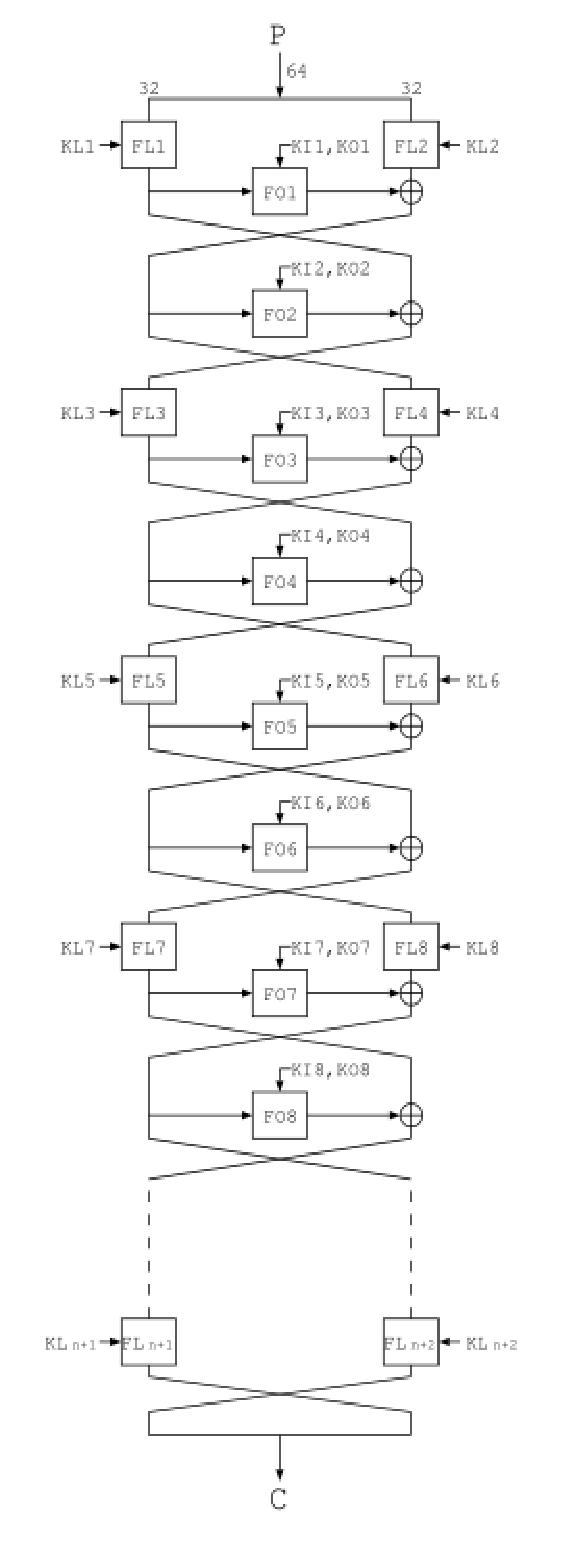
\includegraphics[scale=0.7]{images/misty_feistel}
	\caption{\misty\ cipher structure}
    \label{fig:misty_feistel}
\end{figure}

Key schedule is performed by iterative applying of $FI$ function to each 
$16$-bit chunk of the key (figure~\ref{fig:misty_key_schedule}). Hereby $128$
additional subkey bits are generated.  Both the key and the subkey bits are used
during enciphering.

The key injecting function includes conjunction and disjunction operations and 
is presented on figure~\ref{fig:misty_fl}.

\begin{figure}[p]
    \begin{subfigure}[b]{0.5\textwidth}
        \centering
        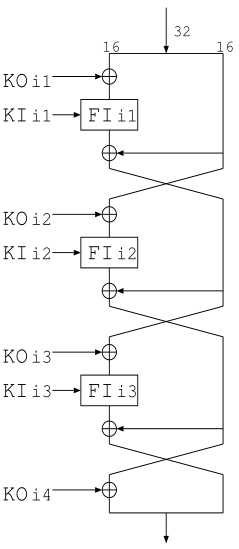
\includegraphics[scale=0.5]{images/misty_fo}
        \caption{$FO$ round function}
        \label{fig:misty_fo}
    \end{subfigure}%
    \begin{subfigure}[b]{0.5\textwidth}
        \centering
        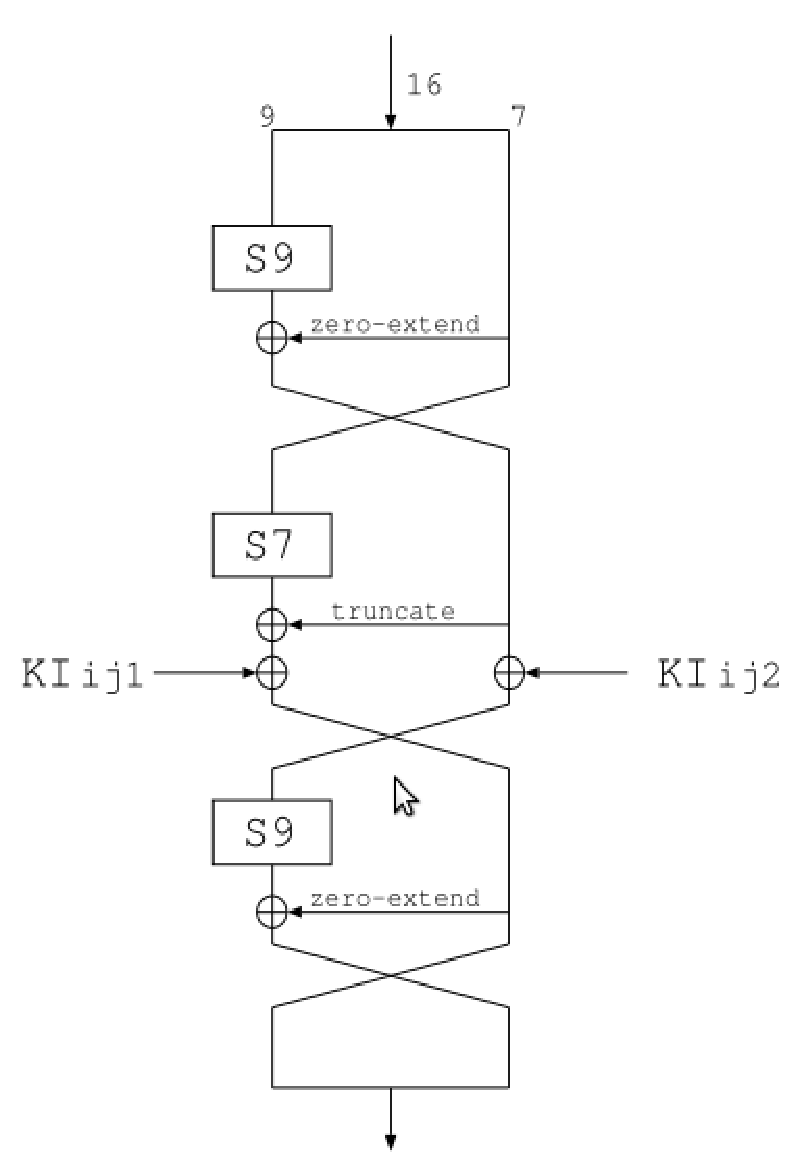
\includegraphics[scale=0.5]{images/misty_fi}
        \caption{$FI$ round function}
        \label{fig:misty_fi}
    \end{subfigure}

    \begin{subfigure}[b]{\textwidth}
        \vspace{1em}
        \centering
        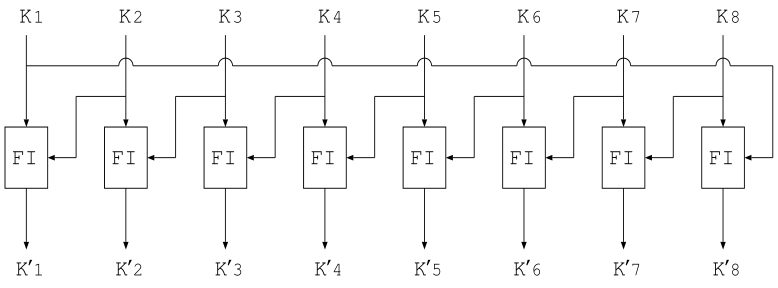
\includegraphics[scale=0.5]{images/misty_key_schedule}
        \caption{Key schedule}
        \label{fig:misty_key_schedule}
    \end{subfigure}
    \caption{\misty\ internal functions}
    \label{fig:misty_round_funcs}
\end{figure}

\begin{figure}[p]
    \centering
    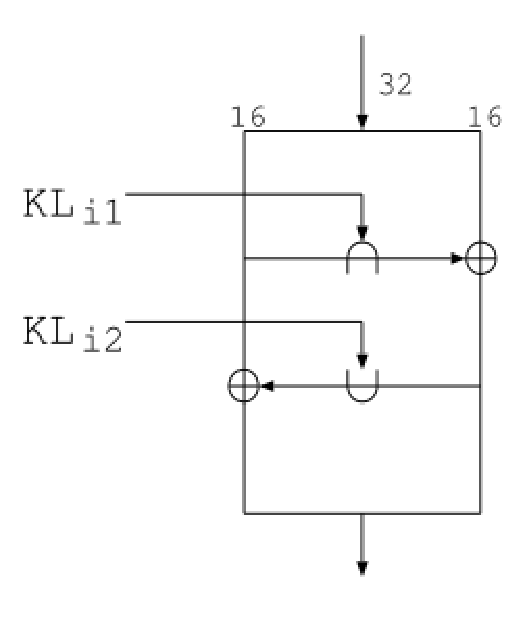
\includegraphics[scale=0.5]{images/misty_fl}
    \caption{Key injection $FL$ function}
    \label{fig:misty_fl}
\end{figure}

S-boxes in \misty\ are constructed algebraically. S-Box $S_7$ has degree $2$ and
$s_9$ is of degree 3. Equations for each S-box are defined in
(\ref{eqn:misty-s7}, \ref{eqn:misty-s9}).

\begin{equation}
    \label{eqn:misty-s7}
    \begin{array}{ll}
        y_0 =& x_0 + x_1 x_3 + x_0 x_3 x_4 + x_1 x_5 + x_0 x_2 x_5 + x_4 x_5 + \\
             & + x_0 x_1 x_6 + x_2 x_6 + x_0 x_5 x_6 + x_3 x_5 x_6 + 1 \\
        y_1 =& x_0 x_2 + x_0 x_4 +x_3 x_4 +x_1 x_5 + x_2 x_4 x_5 +x_6 + \\
             & + x_0 x_6 +x_3 x_6 +x_2 x_3 x_6 + x_1 x_4 x_6 + x_0 x_5 x_6 +1 \\
        y_2 =& x_1 x_2 + x_0 x_2 x_3 + x_4 + x_1 x_4 + x_0 x_1 x_4 + x_0 x_5 + x_0 x_4 x_5 + \\
             & + x_3 x_4 x_5 + x_1 x_6 + x_3 x_6 + x_0 x_3 x_6 + x_4 x_6 + x_2 x_4 x_6 \\
        y_3 =& x_0 + x_1 + x_0 x_1 x_2 + x_0 x_3 + x_2 x_4 + x_1 x_4 x_5 + \\
             & + x_2 x_6 + x_1 x_3 x_6 + x_0 x_4 x_6 + x_5 x_6 + 1 \\ 
        y_4 =& x_2 x_3 + x_0 x_4 + x_1 x_3 x_4 + x_5 + x_2 x_5 + x_1 x_2 x_5 + \\
             & + x_0 x_3 x_5 + x_1 x_6 + x_1 x_5 x_6 + x_4 x_5 x_6 + 1 \\
        y_5 =& x_0 + x_1 + x_2 + x_0 x_1 x_2 + x_0 x_3 + x_1 x_2 x_3 + x_1 x_4 + \\
             & + x_0 x_2 x_4 + x_0 x_5 + x_0 x_1 x_5 + x_3 x_5 + x_0 x_6 + x_2 x_5 x_6 \\
        y_6 =& x_0 x_1 + x_3 + x_0 x_3 + x_2 x_3 x_4 + x_0 x_5 + x_2 x_5 + \\
             & + x_3 x_5 + x_1 x_3 x_5 + x_1 x_6 + x_1 x_2 x_6 + x_0 x_3 x_6 + x_4 x_6 + x_2 x_5 x_6 \\
    \end{array}
\end{equation}

\begin{equation}
    \label{eqn:misty-s9}
    \begin{array}{ll}
        y_0 =& x_0 x_4 + x_0 x_5 + x_1 x_5 + x_1 x_6 + x_2 x_6 + x_2 x_7 + \\
             & + x_3 x_7 + x_3 x_8 + x_4 x_8 + 1 \\
        y_1 =& x_0 x_2 + x_3 + x_1 x_3 + x_2 x_3 + x_3 x_4 + x_4 x_5 + x_0 x_6 + \\
             & + x_2 x_6 + x_7 + x_0 x_8 + x_3 x_8 + x_5 x_8 +1 \\
        y_2 =& x_0 x_1 + x_1 x_3 + x_4 + x_0 x_4 + x_2 x_4 + x_3 x_4 + x_4 x_5 + \\
             & + x_0 x_6 + x_5 x_6 + x_1 x_7 + x_3 x_7 + x_8 \\
        y_3 =& x_0 + x_1 x_2 + x_2 x_4 + x_5 + x_1 x_5 + x_3 x_5 + x_4 x_5 + \\
             & + x_5 x_6 + x_1 x_7 + x_6 x_7 + x_2 x_8 + x_4 x_8 \\
        y_4 =& x_1 + x_0 x_3 + x_2 x_3 + x_0 x_5 + x_3 x_5 + x_6 + x_2 x_6 + \\
             & + x_4 x_6 + x_5 x_6 + x_6 x_7 + x_2 x_8 + x_7 x_8 \\
        y_5 =& x_2 + x_0 x_3 + x_1 x_4 + x_3 x_4 + x_1 x_6 + x_4 x_6 + x_7 + \\
             & + x_3 x_7 + x_5 x_7 + x_6 x_7 + x_0 x_8 + x_7 x_8 \\
        y_6 =& x_0 x_1 + x_3 + x_1 x_4 + x_2 x_5 + x_4 x_5 + x_2 x_7 + x_5 x_7 + \\
             & + x_8 + x_0 x_8 + x_4 x_8 + x_6 x_8 + x_7 x_8 +1 \\
        y_7 =& x_1 + x_0 x_1 + x_1 x_2 + x_2 x_3 + x_0 x_4 + x_5 + x_1 x_6 + \\
             & + x_3 x_6 + x_0 x_7 + x_4 x_7 + x_6 x_7 + x_1 x_8 +1 \\
        y_8 =& x_0 + x_0 x_1 + x_1 x_2 + x_4 + x_0 x_5 + x_2 x_5 + x_3 x_6 + \\
             & + x_5 x_6 + x_0 x_7 + x_0 x_8 + x_3 x_8 + x_6 x_8 +1 \\
    \end{array}
\end{equation}


\section{Construction of equations system for \misty}

\misty is a $64$-bit Feistel network similar to \gost and doesn't use any
additional operations that are not described in~\ref{sec:equations}, there for
construction of equations is performed similarly.

There are few differences however. Even though the transformations used in
\misty\ are resembling those of \gost\, its structure is much more complicated
due to nested Feistel networks. Initially equations for each function are
constructed and tested for correctness so that definition of each Feistel
network is self-contained. Afterwards those equations are chained into single
system as usually.

Since \misty uses key scheduling, equations for this transformation also must be
explicitly defined.

Nested structure of \misty\ results in big number of variables so they must be
named carefully to avoid confusion. The following format was used for \misty\
variables: \verb+R<n>_<func>_<op>_<bit>+, where \verb+n+ denotes number of
current round, \verb+func+ stands for function to which variable belongs, 
\verb+op+ is some operation inside the function, \verb+bit+ is the number of bit
in a block. For example variable \verb+verb+n+ denotes number of
current round, \verb+func+ stands for function to which variable belongs, 
\verb+op+ is some operation inside the function, \verb+bit+ is the number of bit
in a block. For example variable \verb+R5_FO_KO2_15+ stands for round $5$,
function $FO$, operation of injecting subkey $KO_{i2}$, precisely bit $15$ of
the subkey.

Using the described method the full-scale system of equations for \misty\ 
has been constructed and shown to have $3488$ equations in $3680$ variables. 
Because of nested structure too many
variables are introduced and the system becomes underdefined and therefore
unsolvable. To overcome such problem it is possible to apply Gr\"obner basis 
(described in~\ref{sec:groebner}) to some transformation for obtaining more
equations and possibly eliminating some of the variables. It has been decided to
post-process equations for S-box $S_7$ by computing the corresponding
Gr\"obner basis. The resulting system has $8448$ equations in $3680$ variables, 
so usage of Gr\"obner basis introduced another $5000$ equations.


\subsection{Key recovery for 2 rounds of \misty}
\label{sec:misty-key-rec}

For the attack $4$ systems of equations for distinct
\mbox{plaintext/ciphertext} pairs have been combined in order for
the number of known values to reach the unicity distance.

With the use of \verb+CryptoMiniSat+ solver on a low-end computer an equations
system for two \misty\ rounds have successfully been solved and the used subkeys
recovered. For the system of $4$ rounds equivalent keys can be obtained for a
given \mbox{plaintext/ciphertext} pair.

Further combinations of Gr\"obner basis technique with SAT-solvers and
usage of powerful computers may refine the efficiency of the attack and provide
more capabilities for analyzing properties of the cryptoalgorithm.


\section{Summary}

The chapter provides description of constructing systems of non-linear equations
for cryptoalgorithms \gost\ and \misty\ that are based on Feistel network and
some approaches for solving the obtained equations set.

Gr\"obner basis method generally is not efficient enough for solving full-scale
equations system but is useful for obtaining exhaustive list of linearly
independent equations for given transformation. It is especially beneficial for
S-box equations.

With advance of SAT-solver algorithms they become efficient enough for solving
large equations sets and with the help of powerful computers it might be
possible to solve system of equations for some full-scale cipher. The downside
of such algorithms is their nondetermination and therefore no guarantee of
average run time for given instance. This exaggerates complexity evaluation of
solving given equations set and one can only predict the overall complexity of
the problem based on preliminary characteristics of equations set (degree,
number of equations and variables, etc.) and estimate the possibility of its
solving but cannot bind these factors to some certain time complexity of the
attack.

Using the proposed methods for defining symmetric ciphers with equations set,
polynomial system for \misty\ has $8448$ equations in $3680$ variables
and the system for \gost\ has $10432$ equations in $4416$ variables.
For comparison, the polynomial system for the PRESENT cipher that is
designed for lightweight cryptography purposes contains $11067$ quadratic
equations in $4216$ variables~\cite{ches:present:2007}. Even though PRESENT has
very simple structure, its equations system is larger. But also PRESENT has much
smaller key space and requires more space for hardware implementation. It is
claimed that AES cipher can be described with an algebraic system of $8000$
quadratic equations in $1600$ unknowns~\cite{cid2006algebraic} which is
signivicantly smaller than the \gost\ or \misty\ equations system. An equations
set for symmetric block cipher Camellia contains $6224$ equations in $3584$
variables~\cite{Biryukov03blockciphers}.


% AUTHOR: Ruslan Kiianchuk <ruslan.kiianchuk@gmail.com>

\chapter{Description of developed methods for software implementation}
\label{sec:implementation}

\section{Tools and software used for computations}
\label{sec:soft-and-tools}

All computations in this thesis are performed using only free open source
software. The computer algebra system used for algorithm implementations and
experiments is ``SAGE: Software for Algebra and Geometry Experimentation''
which is provided under the terms of the GNU General Public
License~\cite{sage}. SAGE is described as a ``free and open software that
supports research and teaching in algebra, geometry, number theory,
cryptography, etc.''~\cite{sage-core}.

For this thesis the most used components of SAGE were Singular
computer algebra system~\cite{singular}, PolyBoRi C++ library for efficient
reduced Gr\"obener basis computation~\cite{polybori}, and \verb+crypto+ module for cryptography
related routines.


\section{Usage of implemented functionality}
\label{sec:soft-usage}

The implementation architecture of \gost\ cipher and its equation system
generator is inspired by CTC cipher algebraic cryptanalysis description
in~\cite{Albrecht2006}.

Computation of solutions for multivariate algebraic systems of equations is
performed by \mbox{CryptoMiniSat}~\cite{soos:cryptominisat}, a
SAT~Race~2010~\cite{satrace2010} winning SAT solver licensed under GNU Lesser
General Public License.

Conversion of the polynomial system from ANF to CNF format and parsing the
results of \mbox{CryptoMiniSat} computations is done by \verb+anf2cnf.py+
script~\cite{anf2cnf}.


\subsection{\gost\ implementation}
\label{sec:soft-gost}

The \verb+Gost+ class implements \gost\ cryptographic algorithm and its
multivariate quadratic equation system generator. The implementation is not
efficient since it treats every bit as a boolean polynomial ring element, so it
is useful for researching purposes only. 

One can customize \gost\ parameters (like input block size, number of rounds, key
addition mode and subkeys ordering) to get small scale cipher. A cipher instance
compliant with the specification defined in the standard may be constructed as
shown in listing~\ref{lst:spawn_gost}:
\begin{lstlisting}[label=lst:spawn_gost, caption=Creating GOST instance]
sage: gost = Gost(block_size=64, rounds=32, key_add='mod', key_order='frwrev')
sage: print Gost()
GOST cipher (Block Size = 64, Rounds = 32, Key Addition = mod, Key Order = frwrev)
\end{lstlisting}
Those parameters are default and so may be omitted. To create the small scale
version of \gost\ one can specify smaller values for parameters
(listing~\ref{lst:small_gost}):
\begin{lstlisting}[label=lst:small_gost, caption=Small scale GOST]
sage: gost = Gost(block_size=8, rounds=3, key_add='mod', key_order='frw')
sage: print gost.ring
Boolean PolynomialRing in K00, K01, K02, K03, Y00, Y01, Y02, Y03, Z00, Z01, Z02, Z03, K10, K11, K12, K13, Y10, Y11, Y12, Y13, Z10, Z11, Z12, Z13, K20, K21, K22, K23, Y20, Y21, Y22, Y23, Z20, Z21, Z22, Z23, X00, X01, X02, X03, X04, X05, X06, X07, X10, X11, X12, X13, X14, X15, X16, X17, X20, X21, X22, X23, X24, X25, X26, X27, X30, X31, X32, X33, X34, X35, X36, X37
\end{lstlisting}

Cipher variables are defined over boolean polynomial ring. The used notation
is described in section~\ref{seq:key-add-eqn}. In SAGE implementation left digits of the variable index
identify round number and right digits specify the number of bit defined by the
variable. For instance, variable \verb+K0325+ defines 25-th bit of a subkey for round 3. It is
worth noting that for small block sizes the cyclic shift value is
proportionally decreased from 11 bits to 
$\text{ceil}(\text{block\_length} / 3)$,
where $\text{ceil}(x)$ stands for the smallest integer not less than $x$. The
minimum block size is 8 bits since the cipher becomes degenerated with smaller
input blocks.
There are two possible modes for key addition: \verb+mod+ for a standard modular
addition and \verb+xor+ for simple XORing. Also two subkey orderings are
supported: \verb+frwrev+ is for the default ordering when subkeys are reversed on
the last 8 rounds and \verb+frw+ for no reversing. Default S-boxes used in the
cipher are those proposed in GOST~R~31.11-94~\cite{GOST3411} and given in
appendix~\ref{app:gost-sboxes}.

Obtaining polynomial system for \gost\ cryptoalgorithm is shown in
listing~\ref{lst:obtain_sys}:

\begin{lstlisting}[label=lst:obtain_sys, caption=Obtaining polynomial system]
sage: gost = Gost()
sage: gost.polynomial_system()
Polynomial Sequence with 10432 Polynomials in 4416 Variables
\end{lstlisting}


\subsection{\misty\ implementation}

The \verb+Misty+ class implements \misty\ cryptographic algorithm and its
multivariate equations system generator. Its interface is similar to that one of 
\gost. The implementation is not
efficient since it treats every bit as a boolean polynomial ring element, so it
is useful for researching purposes only. 

A required parameter is the number of rounds for the cipher which should be
multiple of $4$ according to the specification. An optional argument is a prefix
that will be prepended to the names of variables for the equations system. This
is used when combining several systems.

An instance of \misty\ polynomial system generator may be created as shown in
listing~\ref{lst:spawn_misty}.
\begin{lstlisting}[label=lst:spawn_misty, caption=Creating MISTY1 instance]
sage: m = Misty(8)         
sage: m.polynomial_system()
Polynomial Sequence with 8448 Polynomials in 3680 Variables
\end{lstlisting}

A decorator \verb+@groebner_basis+ for post-processing the equations via
Gr\"obner basis is implemented and should decorate every function, for which
equations the Gr\"obner basis should be computed as show on
listing~\ref{lst:misty_groebner}).

\begin{lstlisting}[label=lst:misty_groebner, caption=Misty Gr\"obner basis]
     @groebner_basis                                                             
     def s7(self, x, r=None):                                                    
         y = [0] * len(x)
         ...
\end{lstlisting}


\subsection{Solving polynomial systems}
\label{sec:soft-solving}

Obtaining an equation system for the cipher is not enough for recovering an
encryption key. Information about plaintext and ciphertext has to be injected
into equation system by substituting corresponding variables. Also a single
equation system for the specified plaintext and ciphertext does not allow to get a
solution for the key variables, so an ability to combine several equation
systems with different plaintext and ciphertext pairs is needed.

Injecting variable values is implemented by adding new \verb+inject+ method to
a standard \verb+PolynomialSequence_generic+ class and is shown in
listing~\ref{lst:var-inject}.

\begin{lstlisting}[label=lst:var-inject, caption=Injecting variable values into equation system]
sage: gost = Gost(block_size=64, rounds=5, key_add='mod', key_order='frw')             
sage: plaintext = gost.random_block()                                                  
sage: key = gost.random_key()                                                          
sage: ciphertext = gost.encrypt(plaintext, key)                                        
sage: f = gost.polynomial_system()                                                     
sage: print f                                                                        
Polynomial Sequence with 1630 Polynomials in 864 Variables
sage: f2 = f.inject(gost.gen_vars(gost.var_names['block'], 0), plaintext)   
sage: f2 = f2.inject(gost.gen_vars(gost.var_names['block'], 5), ciphertext)
sage: print f2
Polynomial Sequence with 1630 Polynomials in 736 Variables
\end{lstlisting}

For combining several equation systems one should use \verb+join_systems+
function (listing~\ref{lst:combine}) which accepts a list of polynomial systems
with injected known variables and a list of cipher instances for which the
systems were constructed. The function will construct a new boolean polynomial
ring that would include variables from all systems and have the same variables
for encryption subkeys. Consequently, the joined equation systems must contain ciphertexts
obtained on the same key, otherwise combining such systems would not help to
find the solution. In order to distinct variables from different equation systems
one should add a \verb+prefix+ string when constructing a cipher object as
shown in listing~\ref{lst:combine}.
\begin{lstlisting}[label=lst:combine, caption=Combining several equation systems]
sage: gost1 = Gost(block_size=64, rounds=3, key_add='mod', key_order='frw', prefix='a')
sage: gost2 = Gost(block_size=64, rounds=3, key_add='mod', key_order='frw', prefix='b')
sage: plaintext1 = gost1.random_block()                                                
sage: plaintext2 = gost1.random_block()                                                
sage: key = gost1.random_key()                                                         
sage: ciphertext1 = gost1.encrypt(plaintext1, key)                                     
sage: ciphertext2 = gost2.encrypt(plaintext2, key)                                     
sage: f1 = gost1.polynomial_system()                                                   
sage: f2 = gost2.polynomial_system()
sage: f1 = f1.inject(gost1.gen_vars(gost1.var_names['block'], 0), plaintext1)          
sage: f1 = f1.inject(gost1.gen_vars(gost1.var_names['block'], 5), ciphertext1)
sage: f2 = f2.inject(gost2.gen_vars(gost2.var_names['block'], 0), plaintext2) 
sage: f2 = f2.inject(gost2.gen_vars(gost2.var_names['block'], 5), ciphertext2)
sage: f = join_systems([f1, f2], [gost1, gost2])
sage: print f1
Polynomial Sequence with 978 Polynomials in 416 Variables
sage: print f2
Polynomial Sequence with 978 Polynomials in 416 Variables
sage: f1 == f2
False
sage: f = join_systems([f1, f2], [gost1, gost2])                                               
sage: print f
Polynomial Sequence with 1956 Polynomials in 736 Variables
\end{lstlisting}


All functionality for solving the \gost\ and \misty\  polynomial systems is now
implemented.  Two approaches are used for solving equation systems: using
reduced Gr\"obner basis and using SAT solver. 

In listing~\ref{lst:solving-groebner} computing the reduced
Gr\"obner basis for polynomial system is demonstrated. Since all equations in the resulting list
equal 0 it is possible to extract the values of the key bits. In this case the
method allowed to recover only 91 out of 96 subkeys bits for a 3 round GOST
polynomial system.
\begin{lstlisting}[label=lst:solving-groebner, caption=Solving equation system using reduced Gr\"obner basis]
sage: ideal = f.ideal()
sage: basis = ideal.interreduced_basis()
Polynomial Sequence with 735 Polynomials in 736 Variables
sage: key = [i for i in sorted(basis) if str(i).startswith(gost1.var_names['key'])]
sage: print key
[K0229, K0228, K0221, K0220, K0223 + 1, K0222, K0225, K0224, K0227 + 1, K0226, K0131, K0130, K0001, K0000 + 1, K0003, K0002, K0005 + 1, K0004, K0007, K0006, K0009 + bY0009, K0008, K0230 + 1, K0231 + 1, K0126 + 1, K0127 + 1, K0124 + 1, K0125, K0122, K0123, K0120 + bY0009, K0121 + bY0009 + 1, K0128, K0129 + 1, K0012 + 1, K0013, K0010 + 1, K0011 + 1, K0016, K0017, K0014 + 1, K0015, K0018, K0019 + 1, K0203 + 1, K0202 + 1, K0201 + 1, K0200 + 1, K0207 + 1, K0206, K0205 + 1, K0204 + 1, K0209 + 1, K0208 + bY0009 + 1, K0119 + bY0009, K0118, K0117, K0116, K0115 + 1, K0114, K0113, K0112, K0111 + 1, K0110 + 1, K0029 + 1, K0028, K0023 + 1, K0022, K0021 + 1, K0020, K0027, K0026 + 1, K0025 + 1, K0024, K0218 + 1, K0219 + 1, K0214, K0215, K0216 + 1, K0217, K0210, K0211, K0212 + 1, K0213 + 1, K0108, K0109 + 1, K0100 + 1, K0101 + 1, K0102, K0103, K0104, K0105 + 1, K0106, K0107, K0030, K0031]
\end{lstlisting}

For solving an equation system $f$ with CryptoMiniSat solver via SAGE one needs to
install CryptoMiniSat available at~\cite{soos:cryptominisat} first. Then use
\verb+anf2cnf.py+ script provided at~\cite{anf2cnf} for converting the polynomial
system to DIMACS CNF format, call CryptoMiniSat for solving the system and
parse the result back into SAGE as shown in
listing~\ref{lst:solving-sat-example}. In the example the $s$ variable will
store a solution dictionary and $t$ will be initialized by the time needed for
computation.
\begin{lstlisting}[label=lst:solving-sat-example, caption=Solving equation system using SAT solver]
sage: solver = ANFSatSolver(f.ring())
sage: s, t = solver(f)
\end{lstlisting}

\mbox{CryptoMiniSat} solver is more efficient and allows to solve a 6 round GOST
equation system on regular laptop with 2~GHz processor in minutes
(listing~\ref{lst:solving-sat}). Some code is omitted for clarity and is
indicated with dots. Full source code for solving 6 rounds polynomial system is
presented in appendix~\ref{app:solving-sat}. 
\begin{lstlisting}[label=lst:solving-sat, caption=Solving 6 round GOST system using SAT solver]
...
sage: f = join_systems(mqsystems, gosts)
sage: solver = ANFSatSolver(f.ring())
sage: print time.ctime(); s, t = solver(f); print time.ctime();
Sat May 12 22:13:00 2012
Sat May 12 22:13:41 2012
...
sage: print key == recovered_key                                                                             
True
sage: print gosts[0].encrypt(inputs[0],  key) == gosts[0].encrypt(inputs[0], recovered_key) == outputs[0]    
True
\end{lstlisting}

The \misty\ equations system may be solved using Sage interface to available
SAT-solvers (listing~\ref{lst:sat_solve}).
\begin{lstlisting}[label=lst:sat_solve, caption=Using Sage SAT interface]
sage: from sage.sat.boolean_polynomials import solve as sat_solve
sage: m = Misty(4)
sage: F = m.polynomial_system()
sage: print F
Polynomial Sequence with 5156 Polynomials in 2248 Variables
\end{lstlisting}

\section{Summary}

Due to multiple interfaces supported by SAGE it is possible to efficiently
combine various tools for achieving optimal results. In this work the interface
to Singular has been used for computing reduced Gr\"obner basis which managed
to solve 3 round GOST equation system.
\mbox{CryptoMiniSat} solver with \verb+anf2cnf.py+ as a conversion layer
enabled 6 round equation system to be efficiently solved in minutes. There is a
substantial complexity hop for computing 7 rounds, but even though the solution
hasn't been found using regular computer, the memory usage is negligible. So
further optimizations including parallelizing and tweaking SAT algorithm
parameters should result in solving more rounds for GOST~28147 polynomial
system.

Current source code of the \gost\ and \misty\  polynomial system generator is
published by the author at~\cite{zoresvit:repo-algebraic} and the thesis sources
are published at~\cite{zoresvit:thesis}.

\osh
% AUTHOR: Ruslan Kiianchuk <ruslan.kiianchuk@gmail.com>

\Chapter{Conclusions}
\label{sec:conclusions}

As global shift to portable devices usage spawned demand for very efficient and
also secure cryptographic primitives, efficient methods for comprehensive
security evaluation of perspective ciphers are required. Current usage of
insecure ciphers in various fields of information technologies proves the
importance of carefull ciphers security evaluation before deploying them into
real systems.

The accomplished work resulted in development of methods for defining most
widely used cryptographic primitives with system of non-linear equations. The
techniques of obtaining equations for bit permutations, modular addition, some
logical operations and S-boxes should allow to construct full-scale non-linear
equations systems for most modern symmetric ciphers. Best approaches for solving
the obtained equations sets are described and allow to solve reduced round
versions of analyzed ciphers, research algebraic properties of individual
transformations on low-end computers. Usage of resources with more
computational power will increase feasibility of full-scale cipher analysis.

As the result of the work software tools for computational algebra that provide
needed functionality are described and reference implementation for defining
individual transformations with non-linear equations and constructing full-scale
system of equations for modern symmetric ciphers is provided.

An algebraic equation system describing \gost\ cipher and obtained using the
suggested method contains $10432$ polynomials in $4416$ variables. \misty\
cipher is described with $8448$ equations in $3680$ variables using the same
method. Number of equations and variables in \gost system is resembling
that of PRESENT and \misty equations set is larger than that of AES ($3680$
variables in \misty\ against $1600$ variables in AES).

Using the described techniques it is possible to solve a $6$ round
\gost\ polynomial system with $4$ pairs of plaintexts and ciphertexts at the
moment. Thereby the reduced \gost\ algorithm using $160$ out of $256$ key bits is
broken by an algebraic attack. Such statistics strengthens the opinion about
AES vulnerability to algebraic attacks. The
algebraic attack on \misty\ is performed. The equations system for two cipher
round could be solved and equivalent keys for a given
\mbox{plaintext/ciphertext} pair could be found for up to $4$ rounds.
Solving these systems of equations for additional rounds requires more
computation power, however finding the solution may be possible on more
efficient hi-end computers. All computations have been executed on
 \verb+Intel Core i5-3570+ CPU at 3.40~GHz with 8~Gb RAM.

The nondetermination of SAT-solver algorithms do not allow to bind
characteristics of obtained equations set (like its degree, number of equations
and variables, etc.) to some certain time complexity of solving the given
system. However these factors may be used to estimate the feasibility of
solving the system and rationality of allocating processing time for analysis.

Also algebraic analysis in combination with other known cryptanalytic methods
(linear, differential, integral, etc.) proved to be efficient enough for
security evaluation of a cipher~\cite{Albrecht2010}. Considering this practice
algebraic analysis may increase the significance of investigating baby-ciphers
that are shrinked versions of original cryptoalgorithms, so such approach is a
subject for future researches.

\osh{
For labour protection the employee working conditions are analysed for their
compliance with normative documents on safety engineering and sanitaion.
Harmful and dangerous production factors are retrieved and evaluated using the
built ``Human--Machine--Environment'' interaction system. Corresponding safety
measures are developed in order to provide favourable working conditions.
}


\bibliography{references}
% AUTHOR: Ruslan Kiianchuk <ruslan.kiianchuk@gmail.com>

\makeatletter
\renewcommand\chapter{\if@openright\cleardoublepage\else\clearpage\fi
                    \thispagestyle{plain}%
                    \global\@topnum\z@
                    \@afterindentfalse
                    \secdef\@chapter\@schapter}
\def\@chapter[#1]#2{\ifnum \c@secnumdepth >\m@ne
                       \if@mainmatter
                         \refstepcounter{chapter}%
                         \typeout{\@chapapp\space\thechapter.}%
                         \addcontentsline{toc}{chapter}%
                         {\appendixtocname\ \thechapter\ \texorpdfstring{\MakeUppercase{#1}}{#1}}%
                       \else
                       \addcontentsline{toc}{chapter}{\appendixtocname\ \texorpdfstring{\MakeUppercase{#1}}{#1}}%
                       \fi
                    \else
                    \addcontentsline{toc}{chapter}{\appendixtocname\ \texorpdfstring{\MakeUppercase{#1}}{#1}}%
                    \fi
                    \chaptermark{#1}%
                    \addtocontents{lof}{\protect\addvspace{10\p@}}%
                    \addtocontents{lot}{\protect\addvspace{10\p@}}%
                    \if@twocolumn
                      \@topnewpage[\@makechapterhead{#2}]%
                    \else
                      \@makechapterhead{#2}%
                      \@afterheading
                    \fi}
\makeatother


\appendix

\append{GOST~28147-89 equations generator}
\label{app:gost}

\begin{lstlisting}
from copy import deepcopy
from sage.crypto.mq.sbox import SBox
from sage.rings.polynomial.multi_polynomial_sequence import PolynomialSequence
from sage.rings.polynomial.multi_polynomial_sequence import PolynomialSequence_generic


def inject(self, vars, values):
    sub_values = dict(zip(vars, values))
    return self.subs(sub_values)
PolynomialSequence_generic.inject = inject

def join_systems(mqsystems, instances):
    var_names = flatten([i.ring.variable_names() for i in instances])
    common_vars = list(set(var_names))
    common_ring = BooleanPolynomialRing(len(common_vars), common_vars, \
                                        order='degrevlex')
    new_mqsystem = PolynomialSequence([], common_ring)
    for s in mqsystems:
        new_mqsystem.extend(list(s))
    return new_mqsystem


class Gost:
    def _varformatstr(self, name):
        l = str(max([len(str(self.nrounds)), len(str(self.block_size - 1))]))
        return name + "%0" + l + "d" + "%0" + l + "d"

    def _varstrs(self, name, round):
        s = self._varformatstr(name)
        if s.startswith(self.var_names['block']):
            return [s % (round, i) for i in range(self.block_size)]
        else:
            return [s % (round, i) for i in range(self.halfblock_size)]

    def gen_vars(self, name, round_):
        return [self.ring(e) for e in self._varstrs(name, round_)]

    def int2bits(self, num, bits):
        num = Integer(num)
        return num.digits(base=2, padto=Integer(bits))

    def bits2int(self, num_bits):
        num = ''.join([str(i) for i in reversed(num_bits)])
        return int(num, 2)

    def __init__(self, **kwargs):
        self.SBOX_SIZE = 4
        self.nrounds = kwargs.get('rounds', 32)
        if self.nrounds < 8:
            self.key_length = self.nrounds
        else:
            if self.nrounds % 8 != 0:
                raise ValueError('Number of rounds must be multiple of 8')
            self.key_length = 8
        self.block_size = kwargs.get('block_size', 64)
        if self.block_size % self.SBOX_SIZE != 0 or self.block_size < 8:
            raise ValueError('Block size must be multiple of 4 
                    (due to SBox) and greater than 8 (due S-box size)')
        self.halfblock_size = self.block_size / 2
        self.key_order = kwargs.get('key_order', 'frwrev')
        if self.key_order not in ['frw', 'frwrev']:
            raise ValueError('Unsupported key ordering')
        if self.key_order is 'frwrev' and self.nrounds % 8 != 0:
            raise ValueError('frwrev key ordering is only possible 
                    for nrounds to be multiple of 8')
        self.key_add = kwargs.get('key_add', 'mod')
        if self.key_add not in ['mod', 'xor']:
            raise ValueError('key_add may be set to `mod` or `xor`')

        self._init_sboxes(kwargs.get('sboxes', None))
        pre = kwargs.get('prefix', '')
        self.var_names = {'key': 'K', 
                'block': pre + 'X', 
                'sum': pre + 'Y',
                'sbox': pre + 'Z'}
        self.gen_ring()

    def _init_sboxes(self, sboxes):
        self._default_sboxes = [
                [4, 10, 9, 2, 13, 8, 0, 14, 6, 11, 1, 12, 7, 15, 5, 3],
                [14, 11, 4, 12, 6, 13, 15, 10, 2, 3, 8, 1, 0, 7, 5, 9],
                [5, 8, 1, 13, 10, 3, 4, 2, 14, 15, 12, 7, 6, 0, 9, 11],
                [7, 13, 10, 1, 0, 8, 9, 15, 14, 4, 6, 12, 11, 2, 5, 3],
                [6, 12, 7, 1, 5, 15, 13, 8, 4, 10, 9, 14, 0, 3, 11, 2],
                [4, 11, 10, 0, 7, 2, 1, 13, 3, 6, 8, 5, 9, 12, 15, 14],
                [13, 11, 4, 1, 3, 15, 5, 9, 0, 10, 14, 7, 6, 8, 2, 12],
                [1, 15, 13, 0, 5, 7, 10, 4, 9, 2, 3, 14, 6, 11, 8, 12]
                ]
        if not sboxes:
            sboxes = self._default_sboxes
        else:
            for s in sboxes:
                if len(s) != 2 ^ self.SBOX_SIZE: 
                    raise TypeError('S-box must be 4x4 bits (0..15)')
        self.sboxes = [SBox(i, big_endian=False) for i in sboxes]

    def gen_ring(self):
        nr = self.nrounds
        bs = self.block_size
        hbs = self.halfblock_size
        var_names = []
        halfblock_vars = [self.var_names['key'], \
                            self.var_names['sum'], \
                            self.var_names['sbox']]
        for r in range(nr):
            var_names += [self._varformatstr(v) % (r, b) 
                    for v in halfblock_vars for b in xrange(hbs)]
        for r in range(nr + 1):
            var_names += [self._varformatstr(self.var_names['block']) % (r, b) 
                    for b in xrange(bs)]
        self.ring = BooleanPolynomialRing(len(var_names), var_names, \
                                            order='degrevlex') 
        return self.ring

    def polynomial_system(self):
        hbs = self.halfblock_size
        mqsystem_parts = []

        kvars = list()
        for i in range(self.key_length):
            kvars.append(map(self.ring, \
                    self.gen_vars(self.var_names['key'], i)))

        for i in range(self.nrounds):
            xvars = map(self.ring, self.gen_vars(self.var_names['block'], i))
            yvars = map(self.ring, self.gen_vars(self.var_names['sum'], i))
            zvars = map(self.ring, self.gen_vars(self.var_names['sbox'], i))
            next_xvars = map(self.ring, \
                    self.gen_vars(self.var_names['block'], i + 1))
            polynomials = []
            
            if self.key_order == 'frwrev' and \
                    i >= (self.nrounds - self.key_length):
                k = self.key_length - 1 - (i % self.key_length)
            else:
                k = i % self.key_length
            polynomials += self.add_round_key(xvars[:hbs], kvars[k], yvars)
            polynomials += self.polynomials_sbox(yvars, zvars)
            zvars = self.shift(zvars)
            xored = self.xor_blocks(xvars[hbs:], zvars)
            if i < self.nrounds - 1:
                # R_{i+1} = L_i xor f(R_i)
                polynomials += [x + y for x, y in zip(xored, \
                                                        next_xvars[:hbs])]
                # L_{i+1} = R_i
                polynomials += [x + y for x, y in zip(xvars[:hbs], \
                                                        next_xvars[hbs:])]
            else:
                # No block swapping in the last round.
                # R_{i+1} = L_i
                polynomials += [x + y for x, y in zip(xvars[:hbs], \
                                                        next_xvars[:hbs])]
                # L_{i+1} = L_i xor f(R_i)
                polynomials += [x + y for x, y in zip(xored, \
                                                        next_xvars[hbs:])]
            mqsystem_parts.append(polynomials)
        return PolynomialSequence(mqsystem_parts, self.ring)

    def polynomials_sbox(self, yvars, zvars):
        polynomials = list()
        sboxes = deepcopy(self.sboxes)
        for i in range(self.halfblock_size / self.SBOX_SIZE):
            nbit = i * self.SBOX_SIZE
            current_sbox = sboxes[i % len(sboxes)]
            pols = current_sbox.polynomials()
            gens = current_sbox.ring().gens()
            new_gens = yvars[nbit:nbit + self.SBOX_SIZE] + \
                    zvars[nbit:nbit + self.SBOX_SIZE] 
            sub = dict(zip(gens, new_gens))
            pols = [p.subs(sub) for p in pols]
            polynomials += pols
        return polynomials

    def __repr__(self):
        gost_id = 'GOST cipher '
        gost_id += '(Block Size = %d, Rounds = %d, '
        gost_id += 'Key Addition = %s, Key Order = %s)' 
        params = (self.block_size, self.nrounds, self.key_add, self.key_order)
        return gost_id % params

    def add_round_key(self, a, b, r=[]):
        hbs = self.halfblock_size
        is_defined  = lambda vals: all([p.constant() for p in vals])
        # If all variables are defined, just compute the result instead of
        # generating polynomials.
        if is_defined(a) and is_defined(b):
            if self.key_add is 'mod':
                data = self.bits2int(a)
                subkey = self.bits2int(b)
                modulo_mask = (1 << hbs) - 1
                result = (data + subkey) & modulo_mask
                return [self.ring(i) for i in self.int2bits(result, hbs)]
            if self.key_add is 'xor':
                return [x + y for x, y, in zip(a, b)]    
        else:
            if self.key_add is 'mod':
                pols = list()
                pols.append(a[0] + b[0] + r[0]) 
                for i in range(0, hbs - 1):
                    pols.append(a[i] + a[i] * r[i] + a[i] * r[i+1] + a[i] *
                            a[i+1] + a[i] * b[i+1] + r[i] * r[i+1] + r[i] *
                            a[i+1] + r[i] * b[i+1])
                    pols.append(b[i] + b[i] * r[i] + b[i] * r[i+1] + b[i] *
                            a[i+1] + b[i] * b[i+1] + r[i] * r[i+1] + r[i] *
                            a[i+1] + r[i] * b[i+1])
                    pols.append(a[i] * r[i] + b[i] * r[i] + a[i] * b[i] + a[i]
                            + b[i] + r[i+1] + a[i+1] + b[i+1])
                return pols
            if self.key_add is 'xor':
                return [x + y + z for x, y, z in zip(r, a, b)]    

    def shift(self, halfblock):
        shift = ceil(self.halfblock_size / 3)
        halfblock = halfblock[self.halfblock_size-shift:self.halfblock_size]+\ 
                halfblock[0:self.halfblock_size-shift]
        return halfblock

    def substitute(self, halfblock):
        result = []
        for i in range(self.halfblock_size / self.SBOX_SIZE):
            nbit = i * self.SBOX_SIZE
            plain = halfblock[nbit:nbit + self.SBOX_SIZE]
            sub = self.sboxes[i % len(self.sboxes)](plain)
            sub = [self.ring(j) for j in sub]
            result += sub
        return result

    def xor_blocks(self, left, right):
        return [x + y for x, y in zip(left, right)]

    def feistel_round(self, block, subkey):
        hbs = self.halfblock_size
        bs = self.block_size
        n1 = block[0:hbs] # left
        n2 = block[hbs:bs]; # right
        temp = n1
        n1 = self.add_round_key(n1, subkey)
        n1 = self.substitute(n1);
        n1 = self.shift(n1);
        n2 = self.xor_blocks(n1, n2)
        n1 = temp
        return n2 + n1

    def _cast_params(self, data_, key_):
        bs = self.block_size
        data = deepcopy(data_)
        key = deepcopy(key_)
        if not isinstance(data, list):
            data = self.int2bits(data, bs)
        data = [self.ring(i) for i in data]
        if len(key) != self.key_length:
            raise TypeError('Key should be of length ' + str(self.key_length))
        # coerse key bits to ring elements
        for i in range(len(key)):
            if not isinstance(key[i], list):
                key[i] = self.int2bits(key[i], self.halfblock_size)
            key[i] = [self.ring(j) for j in key[i]]
        return data, key

    def encrypt(self, data_, key_):
        hbs = self.halfblock_size
        bs = self.block_size
        if isinstance(data_, list):
            is_list = true;
        else:
            is_list= false;
        data, key = self._cast_params(data_, key_)

        for i in range(self.nrounds):
            if self.key_order == 'frwrev' and \
                    i >= (self.nrounds - self.key_length):
                k = self.key_length - 1 - (i % self.key_length)
            else:
                k = i % self.key_length
            data = self.feistel_round(data, key[k])
        data = data[hbs:bs] + data[0:hbs]
        if is_list:
            return data
        else:
            return self.bits2int(data)

    def decrypt(self, data_, key_):
        hbs = self.halfblock_size
        bs = self.block_size
        if isinstance(data_, list):
            is_list = true;
        else:
            is_list= false;
        data, key = self._cast_params(data_, key_)

        key.reverse()
        for i in range(self.nrounds):
            if self.key_order == 'frwrev' and i < self.key_length:
                k = self.key_length - 1 - (i % self.key_length)
            else:
                k = i % self.key_length
            data = self.feistel_round(data, key[k])
        data = data[hbs:bs] + data[0:hbs]
        if is_list:
            return data
        else:
            return self.bits2int(data)

    def random_key(self):
        key = [list(random_vector(int(self.halfblock_size), x=2)) 
                for _ in range(self.key_length)]
        key = [map(self.ring, i) for i in key]
        return key

    def random_block(self):
        return map(self.ring, list(random_vector(self.block_size, x=2)))

    def test_mqsystem(self, f_):
        if f_.ring() is not self.ring:
            raise TypeError('Tested MQ system has been generated by a ' 
                    'different GOST instance')
        f = deepcopy(f_)
        print 'Testing MQ system', f
        bs = self.block_size
        plaintext = self.random_block()
        key = self.random_key()
        ciphertext = self.int2bits(self.encrypt(plaintext, key), bs)
        f = f.subs(dict(zip(self.gen_vars(self.var_names['block'], \
                                            0), plaintext)))
        f = f.subs(dict(zip(self.gen_vars(self.var_names['block'], \
                                            self.nrounds), ciphertext)))
        for i in range(self.nrounds):
            k = i % self.key_length
            f = f.subs(dict(zip(self.gen_vars(self.var_names['key'], i), \
                                                                key[k])))
        s = f.ideal().interreduced_basis()
        if s == [1]:
            print 'MQ System for' + str(self) + 'is INCORRECT'
            print f
            return False
        else:
            return True


    def test_cipher(self):
        keys = [
                [0x0, 0x0, 0x0, 0x0, 0x0, 0x0, 0x0, 0x0], 
                [0xFFFFFFFF, 0xFFFFFFFF, 0xFFFFFFFF, 0xFFFFFFFF, \
                    0xFFFFFFFF, 0xFFFFFFFF, 0xFFFFFFFF, 0xFFFFFFFF], 
                [0x01234567, 0x89ABCDEF, 0x01234567, 0x89ABCDEF, \
                    0x01234567, 0x89ABCDEF, 0x01234567, 0x89ABCDEF], 
                [0x6ebabf8d, 0x1a8cad60, 0x124744f9, 0xd400b5d8, \
                    0xa721e3fd, 0x11d0702d, 0x06fd4827, 0x476df4bf]
                ]
        plain = [
                0x0000000000000000, 0xBDBDBDBDACACACAC, 0xFFFFFFFFFFFFFFFF, \
                    0x89ABCDEF01234567, 0xC0AE942BC8A99A39
                ]
        cipher = [
                0x12610BE2A6C2FDC9, 0xA587E5D3F6DFB6F4, 0x029BFE67A9364E44, \
                    0x523FC1A6AEC71B9A, 0x780CB7CE063F59E2,
                0x9057C2CF13AAAD6D, 0xF7B085BA4771F406, 0x780416781B29BC06, \
                    0xE596A183FD645558, 0x8EC42736538740AB,
                0xF1956B1D0A1A67DE, 0x9E4C808408DCDBDC, 0x7738AF92DE8FC770, \
                    0x9C44633FCEC0A03E, 0xC23013406002E268,
                0x91DB8E1FE489FAEF, 0x547BF353604A8190, 0x92B517E3CC91B9D0, \
                    0x1F5C2195762513E2, 0xE99D1C8DFF44A74C
                ]

        def show_failed(plain, key, result, expected):
            print 'GOST FAILED'
            print 'key:\t\t', ['0x%8.8X' % subk for subk in key]
            print 'plaintext:\t', "0x%16.16X" % plain
            print 'expected:\t', "0x%16.16X" % expected
            print 'actual:\t\t', "0x%16.16X" % result

        if self.block_size == 64 and self.nrounds == 32 and \
                self.key_add == 'mod' and self.key_order == 'frwrev':
            print 'Testing ', self, 'using test vectors...'
            it = cipher.__iter__()
            for k in keys:
                for p in plain:
                    c = self.encrypt(p, k)
                    expected = it.next() 
                    if c != expected:
                        show_failed(p, k, c, expected)
                        return False
        print 'Testing', self, 'by correct decryption...'
        x = randint(0, 2^self.block_size)
        key = list(random_vector(self.key_length, x = 2^self.block_size))
        c = self.encrypt(x, key)
        d = self.decrypt(c, key)
        if x != d:
            show_failed(x, key, d, x)
            return False
        return True
\end{lstlisting}


\append{Solving 6 rounds of \gost\ \mbox{equations} system}
\label{app:solving-sat}

\begin{lstlisting}
attach gost.sage
attach anf2cnf.py

nr = 5
bs = 64
hbs = int(bs/2)
varnames = ['a', 'b', 'c', 'd']
gosts = [Gost(block_size=bs, 
    rounds=nr, 
    key_add='mod', 
    key_order='frw', 
    prefix=i) for i in varnames]

print 'constructing MQ systems...'
mqsystems = [i.polynomial_system() for i in gosts]

print 'generating plaintext/ciphertext data...'
inputs = [i.random_block() for i in gosts]
key = gosts[0].random_key()
outputs = [gosts[i].encrypt(inputs[i], key) for i in range(len(gosts))]

print  'injecting known variables...'
for i in range(len(mqsystems)):
    mqsystems[i] = mqsystems[i].inject(gosts[i].gen_vars(
            gosts[i].var_names['block'], 0), inputs[i])
    mqsystems[i] = mqsystems[i].inject(gosts[i].gen_vars(
            gosts[i].var_names['block'], nr), outputs[i])

print 'combining MQ systems...'
f = join_systems(mqsystems, gosts)

print 'solving MQ system with SAT solver...'
print time.ctime()
solver = ANFSatSolver(f.ring())
s, t = solver(f)
print 'DONE'
print time.ctime()

recovered_key = []
r = f.ring()
for i in range(len(key)):
    var_names = map(str, gosts[0].gen_vars(
            gosts[0].var_names['key'], i))
    var_names.sort()
    var_names = map(r, var_names)
    recovered_key.append([s[j] for j in var_names])

if gosts[0].int2bits(gosts[0].encrypt(
    inputs[0], recovered_key), bs) == outputs[0]:
    if key == recovered_key:
        print recovered_key
    else:
        print 'FOUND ANOTHER KEY'
        print 'actual'
        print key
        print 'found'
        print recovered_key
\end{lstlisting}


\append{\misty\ equations generator}

\begin{lstlisting}
#!/usr/bin/env sage
# -*- coding: utf-8 -*-

import operator

from sage.rings.polynomial.multi_polynomial_sequence import PolynomialSequence


def split(l, chunk_size):
    """Split flat list into nested lists of length `chunk_size`. If the
    `chunk_size` is not multiple of list length, the last sublist is added as
    is without padding.

    Args:
        l: List to split into chunks.
        chunk_size: Length of a single nested list.

    Returns:
        Nested list of chunks each of the length `chunk_size`.

    """
    return [l[i:i + chunk_size] for i in xrange(0, len(l), chunk_size)]


def reverse(iterable):
    """Return reversed iterable as list."""
    return list(reversed(iterable))


def vector_do(operation, a, b):
    """Perform vector operation on two lists.

    Args:
        operation: binary operation to perform (from `operator` module).
        a: first vector.
        b: second vector.

    Returns:
        Resulting vector (represented as list).

    Example:
        vector_do(operator.__xor__, [1, 1, 1], [1, 0, 1])

    """
    if operation is operator.__xor__:
        if is_constant(a) and is_constant(b):
            return map(lambda x, y: operation(x, y), a, b)
        else:
            # Process variables over Boolean Polynomial Ring correctly.
            return map(lambda x, y: operator.__add__(x, y), a, b)
    elif operation is operator.__and__:
        if is_constant(a) and is_constant(b):
            return map(lambda x, y: operation(x, y), a, b)
        else:
            # Process variables over Boolean Polynomial Ring correctly.
            return map(lambda x, y: operator.__mul__(x, y), a, b)
    elif operation is operator.__or__:
        if is_constant(a) and is_constant(b):
            return map(lambda x, y: operation(x, y), a, b)
        else:
            # Process variables over Boolean Polynomial Ring correctly.
            return map(lambda x, y: x * y + x + y, a, b)
    else:
        return map(lambda x, y: operation(x, y), a, b)


def is_constant(vals):
    """Check of all elements in list are contants, not variables."""
    return all([isinstance(i, Integer) for i in vals])

def groebner_basis(func):
    """Decorator for Groebner basis reduce of polynomial system."""
    def wrapper(*args, **kwargs):
        result = func(*args, **kwargs)
        if not is_constant(result):
            F = PolynomialSequence(result)
            return F.groebner_basis()
        else:
            return result
    return wrapper


class Misty(object):
    """Misty cipher class.

    All method assume to take bit sequences as input. Use `get_bits` method to
    convert integer to Misty bit sequence representation and `get_integer` to
    obtain the corresponding integer back.

    """

    def get_bits(self, integer, nbytes=0):
        """Convert integer to crazy Misty bit ordering. """
        bytes = reverse(integer.digits(256, padto=nbytes))
        bits = [reverse(b.digits(2, padto=8)) for b in bytes]
        return flatten(bits)

    def get_integer(self, bits):
        """Convert crazy Misty bit sequence to sane ordering. """
        bytes = reverse(split(bits, 8))
        bytes = [reverse(b) for b in bytes]
        return Integer(flatten(bytes), 2)

    def __init__(self, nrounds, prefix='', equations_key_schedule=True):
        """Create Misty cipher object.

        It's a full scale cipher as well as its polynomial system generator.

        Args:
            nrounds: Number of enciphering rounds.
            prefix: Prefix used for variables identification during polynomial
                system construction.

        """
        self.nrounds = nrounds
        self.prefix = prefix
        self.equations_key_schedule = equations_key_schedule
        self.block_size = 64
        self.halfblock_size = self.block_size // 2
        self.halfblock_size_fo = self.halfblock_size // 2
        self.fi_left_size = 9
        self.fi_right_size = 7
        self.key = None
        self.subkeys = None
        self.gen_ring()
        # Subkey type constants.
        self.KEY_KO1 = 'ko1'
        self.KEY_KO2 = 'ko2'
        self.KEY_KO3 = 'ko3'
        self.KEY_KO4 = 'ko4'
        self.KEY_KI1 = 'ki1'
        self.KEY_KI2 = 'ki2'
        self.KEY_KI3 = 'ki3'
        self.KEY_KL1 = 'kl1'
        self.KEY_KL2 = 'kl2'

    def kindex(self, subkey_type, i):
        """Index subkey according to crazy Misty indexing rule.

        Args:
            subkey_type: string, indicating subkey type.
            subkeys: list of subkey bits (each element contains 16 subkey
                bits).
            i: Misty round in range 1 <= i <= 8.

        Returns:
            16-bit subkey for corresponding index.
        """
        if i < 1:
            raise ValueError('Subkey index must start from 1. '
                             'Got {0} instead.'.format(i))

        def normalize(x):
            while x > 8:
                x = x - 8
            return x

        if subkey_type == self.KEY_KO1:
            return self.key[i - 1]
        if subkey_type == self.KEY_KO2:
            i = normalize(i + 2)
            return self.key[i - 1]
        if subkey_type == self.KEY_KO3:
            i = normalize(i + 7)
            return self.key[i - 1]
        if subkey_type == self.KEY_KO4:
            i = normalize(i + 4)
            return self.key[i - 1]
        if subkey_type == self.KEY_KI1:
            i = normalize(i + 5)
            return self.subkeys[i - 1]
        if subkey_type == self.KEY_KI2:
            i = normalize(i + 1)
            return self.subkeys[i - 1]
        if subkey_type == self.KEY_KI3:
            i = normalize(i + 3)
            return self.subkeys[i - 1]

        if subkey_type == self.KEY_KL1:
            if i % 2 != 0:
                i = normalize((i + 1) // 2)
                return self.key[i - 1]
            else:
                i = normalize((i // 2) + 2)
                return self.subkeys[i - 1]
        if subkey_type == self.KEY_KL2:
            if i % 2 != 0:
                i = normalize((i + 1) // 2 + 6)
                return self.subkeys[i - 1]
            else:
                i = normalize((i // 2) + 4)
                return self.key[i - 1]

    def fi(self, x, subkey_ki):
        """Misty FI function.

        Args:
            x: 16-bit input value.
            subkey_ki: 16-bit KI key chunk for FI function.

        Returns: 16-bit output of FI function.

        """
        ki7 = subkey_ki[0:self.fi_right_size]
        ki9 = subkey_ki[self.fi_right_size:]

        d9 = x[0:self.fi_left_size]
        d7 = x[self.fi_left_size:]

        d9 = vector_do(operator.__xor__, self.s9(d9), [0, 0] + d7)
        d7 = vector_do(operator.__xor__, self.s7(d7), d9[2:self.fi_left_size])
        d7 = vector_do(operator.__xor__, d7, ki7)
        d9 = vector_do(operator.__xor__, d9, ki9)
        d9 = vector_do(operator.__xor__, self.s9(d9), [0, 0] + d7)
        return d7 + d9

    def key_schedule(self, key):
        """Generate subkeys according to Misty key schedule algorithm.

        Args:
            key: List of 128 bits.

        Returns:
            List of 8 subkeys (each containing list of 16 bits).
        """
        key_chunks = split(key, 16)
        self.key = key_chunks

        subkeys = list()
        for k in range(len(key_chunks)):
            if k < 7:
                subkeys.append(self.fi(key_chunks[k], key_chunks[k + 1]))
            else:
                subkeys.append(self.fi(key_chunks[k], key_chunks[0]))
        self.subkeys = subkeys
        return subkeys

    def fl(self, x, i):
        """Misty key injection FL function.

        Args:
            x: 32-bit input.
            i: number of round.

        Returns:
            Resulting 32 bits after key injection.

        """
        left = x[:self.halfblock_size_fo]
        right = x[self.halfblock_size_fo:]

        kl1 = self.kindex(self.KEY_KL1, i)
        kl2 = self.kindex(self.KEY_KL2, i)

        temp = vector_do(operator.__and__, left, kl1)
        right = vector_do(operator.__xor__, right, temp)

        temp = vector_do(operator.__or__, right, kl2)
        left = vector_do(operator.__xor__, left, temp)
        return left + right

    #@groebner_basis
    def s7(self, x, r=None):
        """Substitute with Misty S7 SBox.

        Bit ordering is reversed due to Crazy Misty Spec bit ordering.
        """
        y = [0] * len(x)
        if not r:
            y[6]  = x[6] ^^x[5] &x[3] ^^x[6] &x[3] &x[2] ^^x[5] &x[1] ^^x[6] &x[4] &x[1] ^^x[2] &x[1] ^^x[6] &x[5] &x[0] ^^x[4] &x[0] ^^x[6] &x[1] &x[0] ^^x[3] &x[1] &x[0] ^^1
            y[5]  = x[6] &x[4] ^^x[6] &x[2] ^^x[3] &x[2] ^^x[5] &x[1] ^^x[4] &x[2] &x[1] ^^x[0] ^^x[6] &x[0] ^^x[3] &x[0] ^^x[4] &x[3] &x[0] ^^x[5] &x[2] &x[0] ^^x[6] &x[1] &x[0] ^^1
            y[4]  = x[5] &x[4] ^^x[6] &x[4] &x[3] ^^x[2] ^^x[5] &x[2] ^^x[6] &x[5] &x[2] ^^x[6] &x[1] ^^x[6] &x[2] &x[1] ^^x[3] &x[2] &x[1] ^^x[5] &x[0] ^^x[3] &x[0] ^^x[6] &x[3] &x[0] ^^x[2] &x[0] ^^x[4] &x[2] &x[0] 
            y[3]  = x[6] ^^x[5] ^^x[6] &x[5] &x[4] ^^x[6] &x[3] ^^x[4] &x[2] ^^x[5] &x[2] &x[1] ^^x[4] &x[0] ^^x[5] &x[3] &x[0] ^^x[6] &x[2] &x[0] ^^x[1] &x[0] ^^1
            y[2]  = x[4] &x[3] ^^x[6] &x[2] ^^x[5] &x[3] &x[2] ^^x[1] ^^x[4] &x[1] ^^x[5] &x[4] &x[1] ^^x[6] &x[3] &x[1] ^^x[5] &x[0] ^^x[5] &x[1] &x[0] ^^x[2] &x[1] &x[0] ^^1
            y[1]  = x[6] ^^x[5] ^^x[4] ^^x[6] &x[5] &x[4] ^^x[6] &x[3] ^^x[5] &x[4] &x[3] ^^x[5] &x[2] ^^x[6] &x[4] &x[2] ^^x[6] &x[1] ^^x[6] &x[5] &x[1] ^^x[3] &x[1] ^^x[6] &x[0] ^^x[4] &x[1] &x[0] 
            y[0]  = x[6] &x[5] ^^x[3] ^^x[6] &x[3] ^^x[4] &x[3] &x[2] ^^x[6] &x[1] ^^x[4] &x[1] ^^x[3] &x[1] ^^x[5] &x[3] &x[1] ^^x[5] &x[0] ^^x[5] &x[4] &x[0] ^^x[6] &x[3] &x[0] ^^x[2] &x[0] ^^x[4] &x[1] &x[0] 
            return y
        else:
            # Process variables over Boolean Polynomial Ring correctly.
            polynomials = [
            r[6] + x[6] + x[5] * x[3] + x[6] * x[3] * x[2] + x[5] * x[1] + x[6] * x[4] * x[1] + x[2] * x[1] + x[6] * x[5] * x[0] + x[4] * x[0] + x[6] * x[1] * x[0] + x[3] * x[1] * x[0] + 1,
            r[5] + x[6] * x[4] + x[6] * x[2] + x[3] * x[2] + x[5] * x[1] + x[4] * x[2] * x[1] + x[0] + x[6] * x[0] + x[3] * x[0] + x[4] * x[3] * x[0] + x[5] * x[2] * x[0] + x[6] * x[1] * x[0] + 1,
            r[4] + x[5] * x[4] + x[6] * x[4] * x[3] + x[2] + x[5] * x[2] + x[6] * x[5] * x[2] + x[6] * x[1] + x[6] * x[2] * x[1] + x[3] * x[2] * x[1] + x[5] * x[0] + x[3] * x[0] + x[6] * x[3] * x[0] + x[2] * x[0] + x[4] * x[2] * x[0],
            r[3] + x[6] + x[5] + x[6] * x[5] * x[4] + x[6] * x[3] + x[4] * x[2] + x[5] * x[2] * x[1] + x[4] * x[0] + x[5] * x[3] * x[0] + x[6] * x[2] * x[0] + x[1] * x[0] + 1,
            r[2] + x[4] * x[3] + x[6] * x[2] + x[5] * x[3] * x[2] + x[1] + x[4] * x[1] + x[5] * x[4] * x[1] + x[6] * x[3] * x[1] + x[5] * x[0] + x[5] * x[1] * x[0] + x[2] * x[1] * x[0] + 1,
            r[1] + x[6] + x[5] + x[4] + x[6] * x[5] * x[4] + x[6] * x[3] + x[5] * x[4] * x[3] + x[5] * x[2] + x[6] * x[4] * x[2] + x[6] * x[1] + x[6] * x[5] * x[1] + x[3] * x[1] + x[6] * x[0] + x[4] * x[1] * x[0],
            r[0] + x[6] * x[5] + x[3] + x[6] * x[3] + x[4] * x[3] * x[2] + x[6] * x[1] + x[4] * x[1] + x[3] * x[1] + x[5] * x[3] * x[1] + x[5] * x[0] + x[5] * x[4] * x[0] + x[6] * x[3] * x[0] + x[2] * x[0] + x[4] * x[1] * x[0]
            ]
            return polynomials


    #@groebner_basis
    def s9(self, x, r=None):
        """Substitute with Misty S9 SBox. """
        y = [0] * len(x)
        if not r:
            y[8] = x[8] &  x[4] ^^ x[8] &  x[3] ^^ x[7] &  x[3] ^^ x[7] &  x[2] ^^ x[6] &  x[2] ^^ x[6] &  x[1] ^^ x[5] &  x[1] ^^ x[5] &  x[0] ^^ x[4] &  x[0] ^^ 1
            y[7] = x[8] &  x[6] ^^ x[5] ^^ x[7] &  x[5] ^^ x[6] &  x[5] ^^ x[5] &  x[4] ^^ x[4] &  x[3] ^^ x[8] &  x[2] ^^ x[6] &  x[2] ^^ x[1] ^^ x[8] &  x[0] ^^ x[5] &  x[0] ^^ x[3] &  x[0] ^^ 1
            y[6] = x[8] &  x[7] ^^ x[7] &  x[5] ^^ x[4] ^^ x[8] &  x[4] ^^ x[6] &  x[4] ^^ x[5] &  x[4] ^^ x[4] &  x[3] ^^ x[8] &  x[2] ^^ x[3] &  x[2] ^^ x[7] &  x[1] ^^ x[5] &  x[1] ^^ x[0]
            y[5] = x[8] ^^ x[7] &  x[6] ^^ x[6] &  x[4] ^^ x[3] ^^ x[7] &  x[3] ^^ x[5] &  x[3] ^^ x[4] &  x[3] ^^ x[3] &  x[2] ^^ x[7] &  x[1] ^^ x[2] &  x[1] ^^ x[6] &  x[0] ^^ x[4] &  x[0]
            y[4] = x[7] ^^ x[8] &  x[5] ^^ x[6] &  x[5] ^^ x[8] &  x[3] ^^ x[5] &  x[3] ^^ x[2] ^^ x[6] &  x[2] ^^ x[4] &  x[2] ^^ x[3] &  x[2] ^^ x[2] &  x[1] ^^ x[6] &  x[0] ^^ x[1] &  x[0]
            y[3] = x[6] ^^ x[8] &  x[5] ^^ x[7] &  x[4] ^^ x[5] &  x[4] ^^ x[7] &  x[2] ^^ x[4] &  x[2] ^^ x[1] ^^ x[5] &  x[1] ^^ x[3] &  x[1] ^^ x[2] &  x[1] ^^ x[8] &  x[0] ^^ x[1] &  x[0]
            y[2] = x[8] &  x[7] ^^ x[5] ^^ x[7] &  x[4] ^^ x[6] &  x[3] ^^ x[4] &  x[3] ^^ x[6] &  x[1] ^^ x[3] &  x[1] ^^ x[0] ^^ x[8] &  x[0] ^^ x[4] &  x[0] ^^ x[2] &  x[0] ^^ x[1] &  x[0] ^^ 1
            y[1] = x[7] ^^ x[8] &  x[7] ^^ x[7] &  x[6] ^^ x[6] &  x[5] ^^ x[8] &  x[4] ^^ x[3] ^^ x[7] &  x[2] ^^ x[5] &  x[2] ^^ x[8] &  x[1] ^^ x[4] &  x[1] ^^ x[2] &  x[1] ^^ x[7] &  x[0] ^^ 1
            y[0] = x[8] ^^ x[8] &  x[7] ^^ x[7] &  x[6] ^^ x[4] ^^ x[8] &  x[3] ^^ x[6] &  x[3] ^^ x[5] &  x[2] ^^ x[3] &  x[2] ^^ x[8] &  x[1] ^^ x[8] &  x[0] ^^ x[5] &  x[0] ^^ x[2] &  x[0] ^^ 1
            return y
        else:
            # Process variables over Boolean Polynomial Ring correctly.
            polynomials = [
            r[8] + x[8] * x[4] + x[8] * x[3] + x[7] * x[3] + x[7] * x[2] + x[6] * x[2] + x[6] * x[1] + x[5] * x[1] + x[5] * x[0] + x[4] * x[0] + 1,
            r[7] + x[8] * x[6] + x[5] + x[7] * x[5] + x[6] * x[5] + x[5] * x[4] + x[4] * x[3] + x[8] * x[2] + x[6] * x[2] + x[1] + x[8] * x[0] + x[5] * x[0] + x[3] * x[0] + 1,
            r[6] + x[8] * x[7] + x[7] * x[5] + x[4] + x[8] * x[4] + x[6] * x[4] + x[5] * x[4] + x[4] * x[3] + x[8] * x[2] + x[3] * x[2] + x[7] * x[1] + x[5] * x[1] + x[0],
            r[5] + x[8] + x[7] * x[6] + x[6] * x[4] + x[3] + x[7] * x[3] + x[5] * x[3] + x[4] * x[3] + x[3] * x[2] + x[7] * x[1] + x[2] * x[1] + x[6] * x[0] + x[4] * x[0],
            r[4] + x[7] + x[8] * x[5] + x[6] * x[5] + x[8] * x[3] + x[5] * x[3] + x[2] + x[6] * x[2] + x[4] * x[2] + x[3] * x[2] + x[2] * x[1] + x[6] * x[0] + x[1] * x[0],
            r[3] + x[6] + x[8] * x[5] + x[7] * x[4] + x[5] * x[4] + x[7] * x[2] + x[4] * x[2] + x[1] + x[5] * x[1] + x[3] * x[1] + x[2] * x[1] + x[8] * x[0] + x[1] * x[0],
            r[2] + x[8] * x[7] + x[5] + x[7] * x[4] + x[6] * x[3] + x[4] * x[3] + x[6] * x[1] + x[3] * x[1] + x[0] + x[8] * x[0] + x[4] * x[0] + x[2] * x[0] + x[1] * x[0] + 1,
            r[1] + x[7] + x[8] * x[7] + x[7] * x[6] + x[6] * x[5] + x[8] * x[4] + x[3] + x[7] * x[2] + x[5] * x[2] + x[8] * x[1] + x[4] * x[1] + x[2] * x[1] + x[7] * x[0] + 1,
            r[0] + x[8] + x[8] * x[7] + x[7] * x[6] + x[4] + x[8] * x[3] + x[6] * x[3] + x[5] * x[2] + x[3] * x[2] + x[8] * x[1] + x[8] * x[0] + x[5] * x[0] + x[2] * x[0] + 1
            ]
            return polynomials

    def fo(self, x, i):
        """Misty FO function.

        Second level nested Feistel network.

        Args:
            x: 32-bit input list.
            i: number of rounds.

        Returns:
            Resulting bits list.
        """


        left = x[0:self.halfblock_size_fo]
        right = x[self.halfblock_size_fo:]

        ki1 = self.kindex(self.KEY_KI1, i)
        ki2 = self.kindex(self.KEY_KI2, i)
        ki3 = self.kindex(self.KEY_KI3, i)

        ko1 = self.kindex(self.KEY_KO1, i)
        ko2 = self.kindex(self.KEY_KO2, i)
        ko3 = self.kindex(self.KEY_KO3, i)
        ko4 = self.kindex(self.KEY_KO4, i)

        left = vector_do(operator.__xor__, left, ko1)
        temp = self.fi(left, ki1)
        left = vector_do(operator.__xor__, temp, right)

        right = vector_do(operator.__xor__, right, ko2)
        temp = self.fi(right, ki2)
        right = vector_do(operator.__xor__, left, temp)

        left = vector_do(operator.__xor__, left, ko3)
        temp = self.fi(left, ki3)
        left = vector_do(operator.__xor__, temp, right)

        right = vector_do(operator.__xor__, right, ko4)

        return right + left

    def feistel_round(self, data, i):
        """Misty Feistel network single run.

        It actually performs first 2 rounds (look for Misty specs).

        Args:
            data: 64-bit input list.
            i: number of actual round (pay attention to indices according
                to Misty specification). Rounds are in range 1 <= i <= n + 2,
                where `n` is total number of rounds
        Returns:
            Resulting 64-bit list.

        """
        left = data[0:self.halfblock_size]
        right = data[self.halfblock_size:]

        # FL1
        left = self.fl(left, i)
        # FL2
        right = self.fl(right, i + 1)

        # FO1
        temp = self.fo(left, i)
        right = vector_do(operator.__xor__, right, temp)

        # FO2
        temp = self.fo(right, i + 1)
        left = vector_do(operator.__xor__, temp, left)

        return left + right

    def encipher(self, data, key):
        """Encipher plaintext with Misty cryptoalgorithm.

        Args:
            data: 64-bit input list (plaintext).
            key: 128-bit input list (key).

        Returns:
            64-bit list (ciphertext).

        """
        for i in range(1, self.nrounds + 1, 2):
            data = self.feistel_round(data, i)

        left = data[0:self.halfblock_size]
        right = data[self.halfblock_size:]
        # FL n+1
        left = self.fl(left, self.nrounds + 1)
        # FL n+2
        right = self.fl(right, self.nrounds + 2)
        return right + left

    def selftest(self):
        """Check Misty test vectors compliance."""
        plaintext = 0x0123456789ABCDEF
        key = 0x00112233445566778899AABBCCDDEEFF
        self.key_schedule(self.get_bits(key, 16))
        c = self.encipher(self.get_bits(plaintext, 8),
                          self.get_bits(key, 16))
        result = self.get_integer(c)
        expected = 0x8b1da5f56ab3d07c
        return result == expected

    def _varformatstr(self, name):
        """Prepare formatting string for variables notation.

        Args:
            name: Variable identificator string.

        Returns:
            Variable identificator string appended with format specificators
            that contains round number and block bit number.
            Format: R<round number>_<var id>_<bit number>

        """
        l = str(len(str(self.block_size - 1)))
        return "R%s_" + name + "_%0" + l + "d"

    def _varstrs(self, name, nbits, round='', start_from=0):
        """Construct strings with variables names.

        Args:
            name: variable string identificator.
            nbits: number of variables set of the same type.
            round: number of round for which variables are defined. If not
                specified, no round prefix is prepended to the string.

        Returns:
            List of strings with variables names.

        """
        round = str(round)
        s = self._varformatstr(name)
        if not round:
            # Exclude round prefix.
            s = s[s.find('_') + 1:]
            var_names = [s % (i) for i in range(start_from, start_from + nbits)]
        else:
            var_names = [s % (round, i) for i in range(start_from, start_from + nbits)]
        if not name == 'K' and not name == 'KS' and not name.startswith('FIKS'):
            # Include polynomial system prefix.
            var_names = [self.prefix + var for var in var_names]
        return var_names

    def vars(self, name, nbits, round='', start_from=0):
        """Construct variables in predefined Misty ring.

        Refer to `_varstrs()` and `gen_ring()` for details.

        """
        var_names = self._varstrs(name, nbits, round=round, start_from=start_from)
        return [self.ring(e) for e in var_names]

    def gen_round_var_names(self, round):
        """Generate variables names set for given round number."""
        var_names = list()
        # FL
        var_names += self._varstrs('FL_KL1', 16, round)
        var_names += self._varstrs('FL_KL2', 16, round)
        var_names += self._varstrs('FL_XOR', 16, round)
        var_names += self._varstrs('FL', 32, round)
        # FI
        for i in range(1, 4):
            # FI has 3 subrounds in FO function.
            var_names += self._varstrs('FI' + str(i), 16, round)
            var_names += self._varstrs('FI' + str(i) + '_S9', 9, round)
            var_names += self._varstrs('FI' + str(i) + '_S7', 7, round)
            var_names += self._varstrs('FI' + str(i) + '_SS9', 9, round)
            var_names += self._varstrs('FI' + str(i) + '_KI2', 16, round)
        # FO
        var_names += self._varstrs('FO', 32, round)
        var_names += self._varstrs('FO_KO1', 16, round)
        var_names += self._varstrs('FO_KO2', 16, round)
        var_names += self._varstrs('FO_KO3', 16, round)


        return var_names

    def gen_ring(self):
        """Generate ring for Misty polynomial equations system.

        Construct all variables needed for describing Misty cryptoalgorithm
        with polynomial equations system and generate the corresponding
        Boolean Polynomial Ring.

        """
        var_names = list()

        # Input plaintext.
        var_names += self._varstrs('IN', 64)
        # Output ciphertext.
        var_names += self._varstrs('OUT', 64)

        # Key variables.
        var_names += self._varstrs('K', 128)
        # Subkey variables.
        var_names += self._varstrs('KS', 128)

        if self.equations_key_schedule == True:
            for i in range(8):
                var_names += self._varstrs('FIKS' + str(i), 16)
                var_names += self._varstrs('FIKS' + str(i) + '_S9', 9)
                var_names += self._varstrs('FIKS' + str(i) + '_S7', 7)
                var_names += self._varstrs('FIKS' + str(i) + '_SS9', 9)
                var_names += self._varstrs('FIKS' + str(i) + '_KI2', 16)

        for i in range(1, self.nrounds + 1):
            var_names += self.gen_round_var_names(i)
        for i in range(1, self.nrounds + 1):
            if i % 2 == 1:
                var_names += self._varstrs('FX', 32, i)
            else:
                var_names += self._varstrs('F', 64, i)
        for i in range(self.nrounds + 1, self.nrounds + 3):
            # FL
            var_names += self._varstrs('FL_KL1', 16, i)
            var_names += self._varstrs('FL_KL2', 16, i)
            var_names += self._varstrs('FL_XOR', 16, i)
            var_names += self._varstrs('FL', 32, i)

        self.ring = BooleanPolynomialRing(len(var_names), var_names, order='degrevlex')


    def polynomials_fl(self, x, i):
        """Construct polynomials for Misty FL function."""

        left = x[:self.halfblock_size_fo]
        right = x[self.halfblock_size_fo:]

        kl1 = self.kindex(self.KEY_KL1, i)
        kl2 = self.kindex(self.KEY_KL2, i)

        polynomials = list()

        ## Generate variables for given round
        vars_kl1 = self.vars('FL_KL1', 16, i)
        vars_kl2 = self.vars('FL_KL2', 16, i)
        vars_xor = self.vars('FL_XOR', 16, i)
        vars_out = self.vars('FL', 32, i)

        temp = vector_do(operator.__and__, left, kl1)
        polynomials.extend(vector_do(operator.__xor__, temp, vars_kl1))

        right = vector_do(operator.__xor__, right, vars_kl1)
        polynomials.extend(vector_do(operator.__xor__, right, vars_xor))

        # Replace `x or y` operation with equivalent `x * y ^ x + y`.
        temp = vector_do(operator.__or__, vars_xor, kl2)
        polynomials.extend(vector_do(operator.__xor__, temp, vars_kl2))

        left = vector_do(operator.__xor__, left, vars_kl2)
        polynomials.extend(vector_do(operator.__xor__, left, vars_out[0:16]))
        polynomials.extend(vector_do(operator.__xor__, vars_xor, vars_out[16:32]))

        return flatten(polynomials)

    def polynomials_fi(self, x, subkey_ki, subround, r=''):
        """Construct polynomials for Misty FI function.

        Args:
            x: list of 16 input variables.
            subkey_ki: 16-bit key chunk.
            subround: number of FI round in FO function (1..3).
            r: number of actual outer Feistel network enciphering round.

        """
        ki7 = subkey_ki[0:self.fi_right_size]
        ki9 = subkey_ki[self.fi_right_size:]

        d9 = x[0:self.fi_left_size]
        d7 = x[self.fi_left_size:]

        subround = str(subround)

        if subround in ['1', '2', '3']:
            vars_fi = self.vars('FI' + subround, 16, r)
        else:
            vars_fi = self.vars('KS', 16, start_from=int(subround[2]) * 16)

        vars_s9 = self.vars('FI' + subround + '_S9', 9, r)
        vars_s7 = self.vars('FI' + subround + '_S7', 7, r)
        vars_ss9 = self.vars('FI' + subround + '_SS9', 9, r)
        vars_ki2 = self.vars('FI' + subround + '_KI2', 9, r)

        polynomials = list()
        pad = [self.ring(0)] * 2

        polynomials.extend(self.s9(d9, vars_s9))
        d9 = vector_do(operator.__xor__, vars_s9, pad + d7) # add to pols

        polynomials.extend(self.s7(d7, vars_s7))
        d7 = vector_do(operator.__xor__, vars_s7, d9[2:self.fi_left_size]) # add to pols
        d7 = vector_do(operator.__xor__, d7, ki7)

        d9 = vector_do(operator.__xor__, d9, ki9)
        polynomials.extend(vector_do(operator.__xor__, d9, vars_ki2))

        polynomials.extend(self.s9(vars_ki2, vars_ss9))
        d9 = vector_do(operator.__xor__, vars_ss9, pad + d7) # add to pols

        polynomials.extend(vector_do(operator.__xor__, vars_fi[0:7], d7))
        polynomials.extend(vector_do(operator.__xor__, vars_fi[7:16], d9))
        return polynomials

    def polynomials_fo(self, x, i):
        """Construct polynomials for Misty FI function."""

        left = x[0:self.halfblock_size_fo]
        right = x[self.halfblock_size_fo:]

        ki1 = self.kindex(self.KEY_KI1, i)
        ki2 = self.kindex(self.KEY_KI2, i)
        ki3 = self.kindex(self.KEY_KI3, i)

        ko1 = self.kindex(self.KEY_KO1, i)
        ko2 = self.kindex(self.KEY_KO2, i)
        ko3 = self.kindex(self.KEY_KO3, i)
        ko4 = self.kindex(self.KEY_KO4, i)

        vars_fo = self.vars('FO', 32, i)
        vars_ko1 = self.vars('FO_KO1', 16, i)
        vars_ko2 = self.vars('FO_KO2', 16, i)
        vars_ko3 = self.vars('FO_KO3', 16, i)
        vars_fi1 = self.vars('FI1', 16, i)
        vars_fi2 = self.vars('FI2', 16, i)
        vars_fi3 = self.vars('FI3', 16, i)

        polynomials = list()

        left = vector_do(operator.__xor__, left, ko1)
        polynomials.extend(vector_do(operator.__xor__, left, vars_ko1))
        polynomials.extend(self.polynomials_fi(vars_ko1, ki1, 1, i))  # FI1 variables introduced.
        left = vector_do(operator.__xor__, vars_fi1, right)

        right = vector_do(operator.__xor__, right, ko2)
        polynomials.extend(vector_do(operator.__xor__, right, vars_ko2))
        polynomials.extend(self.polynomials_fi(vars_ko2, ki2, 2, i))  # FI2 variables introduced.
        right = vector_do(operator.__xor__, vars_fi2, left)

        left = vector_do(operator.__xor__, left, ko3)
        polynomials.extend(vector_do(operator.__xor__, left, vars_ko3))
        polynomials.extend(self.polynomials_fi(vars_ko3, ki3, 3, i))  # FI3 variables introduced.
        left = vector_do(operator.__xor__, vars_fi3, right)

        right = vector_do(operator.__xor__, right, ko4)
        polynomials.extend(vector_do(operator.__xor__, right, vars_fo[0:16]))
        polynomials.extend(vector_do(operator.__xor__, left, vars_fo[16:32]))

        return polynomials

    def polynomials_round(self, data, i):
        """Construct polynomials for Misty Feistel single run."""
        left = data[0:self.halfblock_size]
        right = data[self.halfblock_size:]

        vars_fl1 = self.vars('FL', 32, i)
        vars_fl2 = self.vars('FL', 32, i + 1)
        vars_fo1 = self.vars('FO', 32, i)
        vars_fo2 = self.vars('FO', 32, i + 1)
        vars_fx = self.vars('FX', 32, i)
        vars_f = self.vars('F', 64, i + 1)

        polynomials = list()

        polynomials.extend(self.polynomials_fl(left, i))  # FL1 fariables introduced.
        polynomials.extend(self.polynomials_fl(right, i + 1))  # FL2 fariables introduced.

        polynomials.extend(self.polynomials_fo(vars_fl1, i))  # FO1 variables introduced.
        right = vector_do(operator.__xor__, vars_fo1, vars_fl2)
        polynomials.extend(vector_do(operator.__xor__, right, vars_fx))

        polynomials.extend(self.polynomials_fo(vars_fx, i + 1))  # FO2 variables introduced.
        left = vector_do(operator.__xor__, vars_fo2, vars_fl1)
        polynomials.extend(vector_do(operator.__xor__, left, vars_f[0:32]))
        polynomials.extend(vector_do(operator.__xor__, vars_fx, vars_f[32:64]))

        return polynomials

    def polynomials_key_schedule(self):
        """Construct polynomials for Misty key scheduling."""
        self.key = split(self.vars('K', 128), 16)

        polynomials = list()
        for k in range(len(self.key)):
            subround = 'KS' + str(k)
            if k < 7:
                polynomials.extend(self.polynomials_fi(self.key[k], self.key[k + 1], subround))
            else:
                polynomials.extend(self.polynomials_fi(self.key[k], self.key[0], subround))
        self.subkeys = split(self.vars('KS', 128), 16)
        return polynomials

    def polynomial_system(self):
        """Construct polynomials system for Misty cipher."""
        polynomials = list()

        plain = self.vars('IN', 64)
        if self.equations_key_schedule is True:
            polynomials.extend(self.polynomials_key_schedule())
        else:
            self.key = split(self.vars('K', 128), 16)
            self.subkeys = split(self.vars('KS', 128), 16)

        polynomials.extend(self.polynomials_round(plain, 1))  # R2_F variables introduced.
        for i in range(3, self.nrounds + 1, 2):
            vars_f_prev = self.vars('F', 64, i - 1)
            polynomials.extend(self.polynomials_round(vars_f_prev, i))

        vars_f = self.vars('F', 64, self.nrounds)
        vars_fl1 = self.vars('FL', 32, self.nrounds + 1)
        vars_fl2 = self.vars('FL', 32, self.nrounds + 2)
        vars_out = self.vars('OUT', 64)

        left = vars_f[0:self.halfblock_size]
        right = vars_f[self.halfblock_size:]

        polynomials.extend(self.polynomials_fl(left,  self.nrounds + 1))
        polynomials.extend(self.polynomials_fl(right,  self.nrounds + 2))
        polynomials.extend(vector_do(operator.__xor__, vars_fl1, vars_out[32:64]))
        polynomials.extend(vector_do(operator.__xor__, vars_fl2, vars_out[0:32]))
        return PolynomialSequence(polynomials)
\end{lstlisting}


\append{Solving 2 rounds of \misty\ equations system}
\label{app:misty-solve}

\begin{lstlisting}
from sage.rings.polynomial.multi_polynomial_sequence import PolynomialSequence
from sage.rings.polynomial.multi_polynomial_sequence import PolynomialSequence_generic

from sage.sat.boolean_polynomials import solve as sat_solve

load('misty.sage')

def inject_vars(F, vars, values):
    """Inject vars values into polynomial system. """
    sub_values = dict(zip(vars, values))
    return F.subs(sub_values)


def get_vars(solution, vars):
    """Obtain variable values from solution dict. """
    var_names = map(str, vars)
    solution = dict(zip(map(str, solution.keys()), solution.values()))
    values = list()
    for i in var_names:
        values.append(solution.get(i))
    return values


def join_systems(mqsystems):
    """Join polynomial systems into one.

    Key variables aren't prefixed since they must be the same through all
    systems. Joined systems with different keys injected are incorrect.

    """
    var_names = flatten([system.ring().variable_names() for system in mqsystems])
    common_vars = list(set(var_names))
    common_ring = BooleanPolynomialRing(len(common_vars), common_vars, order='degrevlex')
    new_mqsystem = PolynomialSequence([], common_ring)
    for s in mqsystems:
        new_mqsystem.extend(list(s))
    return new_mqsystem

def solve_single_system():
    m = Misty(2)
    plaintext = [1] * 64
    key = [1] * 128
    m.key_schedule(key)
    ciphertext = m.encipher(plaintext, key)

    print 'constructing polynomials...'
    polynomials = m.polynomial_system()
    print 'constructing equations system...'
    F = PolynomialSequence(polynomials)
    print 'injecting variables...'
    F = inject_vars(F, m.vars('IN', 64), plaintext)
    F = inject_vars(F, m.vars('OUT', 64), ciphertext)
    print 'solving system...'
    result = sat_solve(F)
    print 'Done.'
    key = get_vars(result[0], m.vars('K', 128))
    print key


def solve_joined_systems():
    nrounds = 2
    instances = [Misty(nrounds, prefix) for prefix in ['a', 'b']]

    print 'constructing equation systems...'
    eqsystems = [i.polynomial_system() for i in instances]

    inputs = [[0] * 64, [1] * 64]
    key = [1] * 128
    outputs = list()
    for i, m in enumerate(instances):
        m.key_schedule(key)
        outputs.append(m.encipher(inputs[i], key))
    print 'INPUTS:'
    for i in inputs:
        print hex(instances[0].get_integer(i))
    print 'KEY:'
    print hex(instances[0].get_integer(key))
    print 'OUTPUTS:'
    for i in outputs:
        print hex(instances[0].get_integer(i))

    print '\ninjecting known variables...'
    for i, m in enumerate(instances):
        eqsystems[i] = inject_vars(eqsystems[i], m.vars('IN', 64), inputs[i])
        eqsystems[i] = inject_vars(eqsystems[i], m.vars('OUT', 64), outputs[i])

    for i in eqsystems:
        print i.__str__()

    print '\ncombining equation systems...'
    eqsystem = join_systems(eqsystems)
    print eqsystem.__str__()

    print '\nsolving equation system...'
    solution = sat_solve(eqsystem)[0]
    print solution

\end{lstlisting}

\append{S-boxes for GOST~28147-89 implementation}
\label{app:gost-sboxes}

\begin{equation}
    \nonumber
    \begin{array}{lllllllllllllllll}
        S_1 =&  \{4, &  10, &  9, &  2, &  13, &  8, &  0, &  14, &  6, &  11, &  1, &  12, &  7, &  15, &  5, &  3 \} \\
        S_2 =&  \{14, &  11, &  4, &  12, &  6, &  13, &  15, &  10, &  2, &  3, &  8, &  1, &  0, &  7, &  5, &  9 \} \\
        S_3 =&  \{5, &  8, &  1, &  13, &  10, &  3, &  4, &  2, &  14, &  15, &  12, &  7, &  6, &  0, &  9, &  11 \} \\
        S_4 =&  \{7, &  13, &  10, &  1, &  0, &  8, &  9, &  15, &  14, &  4, &  6, &  12, &  11, &  2, &  5, &  3 \} \\
        S_5 =&  \{6, &  12, &  7, &  1, &  5, &  15, &  13, &  8, &  4, &  10, &  9, &  14, &  0, &  3, &  11, &  2 \} \\
        S_6 =&  \{4, &  11, &  10, &  0, &  7, &  2, &  1, &  13, &  3, &  6, &  8, &  5, &  9, &  12, &  15, &  14 \} \\
        S_7 =&  \{13, &  11, &  4, &  1, &  3, &  15, &  5, &  9, &  0, &  10, &  14, &  7, &  6, &  8, &  2, &  12 \} \\
        S_8 =&  \{1, &  15, &  13, &  0, &  5, &  7, &  10, &  4, &  9, &  2, &  3, &  14, &  6, &  11, &  8, &  12 \}
    \end{array}
\end{equation}

\append{List of publications}

\begingroup
\renewcommand{\chapter}[2]{}%
\begin{thebibliography}{1}
\renewcommand{\cyrdash}{}
\providecommand*{\BibEmph}[1]{#1}
\providecommand*{\BibDash}{\ifdim\lastskip>0pt\unskip\nobreak\hskip.2em\fi\cyrdash\hskip.2em\ignorespaces}

\bibitem{Kiyanchuk:DESSERT:2012}
\BibEmph{Oliynykov~R.~V., Kiyanchuk~R.~I.} {Perspective Symmetric Block Cipher
  optimized for Hardware Implementation}~// {6-th International Conference
  ``Dependable Systems, Services \& Technologies (DESSERT'12)''}. \BibDash
\newblock 2012.

\bibitem{Kiyanchuk:visnyk:2012}
\BibEmph{Kiyanchuk~R.~I., Oliynykov~R.~V.} {Linear transformation properties of
  ZUC cipher}~// \BibEmph{Visnyk}. \BibDash
\newblock 2012. \BibDash
\newblock {Mathematical modeling. Information technologies. Computer-aided
  control systems.}

\bibitem{karazina:zuc}
\BibEmph{{Kiyanchuk, R. I. and Oliynykov R. V.}} {Linear transformation
  properties of ZUC cipher}~// {Computer modeling in high-end technologies}~/
  Kharkiv national university of radio electronics. \BibDash
\newblock {Kharkiv}, 2012. \BibDash
\newblock P.~199 -- 202.

\bibitem{Kiyanchuk:2012:Banking}
\BibEmph{Kiyanchuk~R.~I.} {Differential analysis of S-functions
  [In~Russian]}~// {Scientific youth researching for European integration}~/
  Kharkiv university of banking. \BibDash
\newblock Kharkiv, 2012. \BibDash
\newblock Electronic resource on CD-ROM.

\bibitem{Kiyanchuk:2012:MMF}
\BibEmph{Kiyanchuk~R.~I.} {Differential analysis of S-functions
  [In~Russian]}~// {Radioelectronics and youth in XXI century}~/ Kharkiv
  national university of radio electronics. \BibDash
\newblock Kharkiv, 2012. \BibDash
\newblock {P.}~130 -- 131.

\bibitem{Kiyanchuk:2011:MMF}
\BibEmph{Kiyanchuk~R.~I.} {Comparative analysis of IDEA-like Block Symmetric
  Ciphers [In~Ukrainian]}~// {International Conference ``Computer
  Engineering''}~/ {Kharkiv National University of Radio Electronics}. \BibDash
\newblock Vol.~5. \BibDash
\newblock Kharkiv, 2011. \BibDash April. \BibDash
\newblock {P.}~225 -- 227.

\bibitem{Kiyanchuk:IREF:2011:present}
\BibEmph{Oliynykov~R.~V., Kiyanchuk~R.~I.} {Perspective Symmetric Block Cipher
  Optimized for Hardware Implementation [In~Russian]}~// {``Telecommunication
  Systems and Technologies''}~/ {Kharkiv National University of Radio
  Electronics}. \BibDash
\newblock Vol.~II. \BibDash
\newblock {Kharkiv, Ukraine}, 2011. \BibDash October. \BibDash
\newblock P.~321 -- 330.

\bibitem{Kiyanchuk:2011:Customs}
\BibEmph{Oliynykov~R.~V., Kiyanchuk~R.~I.} {Usage of T-functions in Symmetric
  Cryptographic Transformations [In~Russian]}~// {``Perspectives of Information
  and transport-customs technologies in customs affairs, external economic
  industry and organizations management''}~/ {Kharkiv National University of
  Radio Electronics}. \BibDash
\newblock Dnipropetrovs'k, 2011. \BibDash December. \BibDash
\newblock {P.}~213 -- 215. \BibDash
\newblock Section 2.

\bibitem{Kiyanchuk:2009:rijndael}
\BibEmph{Dolgov~V.~I., Lysytska~I.~V., Kiyanchuk~R.~I.} {RIJNDAEL -- Is This a
  New or Well Forgotten Old Solution? [In~Russian]}~// {Computer Science and
  Technologies}~/ {Kharkiv National University of Radio Electronics}. \BibDash
\newblock 2009. \BibDash
\newblock P.~32 -- 35.

\bibitem{Kiyanchuk:2012:kyiv}
\BibEmph{Oliynykov R. V., Kiyanchuk R. I., Gorbenko I. D.}
\newblock {Algebraic cryptanalysis of \gost}~ 
\newblock {XV Internationa scientifically-practical conference 22--25 May, -- 2012}~/ 
Kharkiv National University of Radio and Electronics. \BibDash Kyiv, 2012. \BibDash {P.}~130 -- 131.

\bibitem{Kiyanchuk:2013:MMF}
\BibEmph{Kiyanchuk~R.~I.} \newblock {Algebraic cryptanalysis of \gost}~ 
\newblock {Radioelectronics and youth in XXI century}~/ 
Kharkiv National University of Radio and Electronics.\BibDash Kharkiv, 2013. \BibDash {P.}~119 -- 120.

\end{thebibliography}
\endgroup


\end{document}
